\documentclass[12pt,a4paper]{article}

% --- Standard Packages ---
\usepackage[utf8]{inputenc}
\usepackage[english]{babel}
\usepackage[T1]{fontenc}
\usepackage{geometry}
\geometry{margin=2.0cm}
\usepackage{graphicx}
\usepackage[absolute,overlay]{textpos}
\usepackage[table]{xcolor}
\usepackage{hyperref}
\usepackage{enumitem}
\usepackage{amsmath, amssymb}
\usepackage{booktabs}
\usepackage{multirow}
\usepackage{float}
\usepackage{subcaption}
\usepackage[capitalise,noabbrev]{cleveref}

% --- Custom packages for table auto-sizing and wrapping ---
\usepackage{tabularx}
\newcolumntype{L}{>{\raggedright\arraybackslash}X}

\hypersetup{
    colorlinks=true,
    linkcolor=blue!60!black,
    citecolor=blue!60!black,
    urlcolor=blue!60!black,
}

% --- Document Information ---
\title{%
    Contextual Football Scouting\\[4pt]
    \large Mitigating Team Bias via 360 Spatial Data Analysis%
}
\author{Matteo Vezzoli \& Armando Mio}
\date{June 2026}

\begin{document}

\begin{textblock*}{6cm}(10mm, 10mm)
    
\includegraphics[width=6cm]{../logo.png}
\end{textblock*}

\maketitle

% ============================================================
% ABSTRACT
% ============================================================
\begin{abstract}
Traditional scouting statistics reward volume (passes played, distance covered, touches taken) and in doing so carry a heavy \textbf{team bias}: a midfielder in a possession-dominant side piles up numbers a better player in a pressed side never gets the chance to produce. The effect is large and easy to miss. On a contextual measure of the value a player actually creates, more than half of the Euro~2024 player pool moves by 20 or more percentile points versus a volume-based ranking. Phil Foden, for instance, sits in the 89th percentile of wingers for passing volume but the 11th for value created, while Tom\'{a}\v{s} Sou\v{c}ek does the opposite (3rd for volume, 83rd for value).

This project reframes player evaluation around \emph{what a player does with the space around him}, read from \textbf{StatsBomb~360 freeze frames} rather than the event log alone, and graded by the value of each action rather than its frequency. Two design choices unify the work: \textbf{Expected Possession Value~(EPV)} as the common currency, and \textbf{within-role percentiles} as the common lens (a centre-back is ranked only against other centre-backs). One enabler is methodological. A 360 frame shows where players are but \textbf{not who they are}, so we build a resolver that puts identities back on the anonymous dots; it is validated at 93\% accuracy against the one place ground truth exists, completed passes, and then carried to the off-ball runs where no ground truth is available.

On this basis we present four validated studies on the same pool of 272 players: (H1)~\textbf{Space Control~\&~Value}, a four-index spatial profile; (H2)~\textbf{Decision Quality}, the value of the pass chosen against the in-frame options ignored; (H3)~\textbf{Off-Ball Movement}, the dangerous off-ball space a player offers that teammates fail to use; and (H4)~\textbf{Player Similarity}, matching players by their contextual ``spatial DNA'' to surface cheaper look-alikes. Beyond confirming what football already knows, the metrics isolate a previously invisible signal, the ``shadow runner'' who keeps offering dangerous options his team never plays, with Pedri the clearest case of the tournament. The four studies feed an interactive scouting dashboard.
\end{abstract}

\vfill
\begin{center}
\small
\setlength{\tabcolsep}{0pt}
\begin{tabular}{@{}p{3.2cm}@{\hspace{1em}}l@{}}
\textbf{Live dashboard:} & \url{https://contextual-football-scouting.vercel.app/} \\[4pt]
\textbf{Source code:}    & \url{https://github.com/ArMat-Analytics/Contextual-Football-Scouting} \\
\end{tabular}
\end{center}
\vspace{2em}

\clearpage
% ============================================================
\section{Introduction and Motivation}\label{sec:intro}
% ============================================================

\subsection{The Problem: Team Bias}\label{sec:team-bias}

In the modern transfer market, clubs frequently overvalue players on the basis of superficial statistical output.
Very often those inflated numbers are a by-product of the player operating inside a dominant team structure, not a reflection of exceptional individual talent.
A midfielder in a possession-dominant team will inevitably register a high pass-completion rate; but if those passes are played under little pressure and carry little complexity, they say little about elite passing ability.

The central challenge of football scouting today is therefore the phenomenon known as \textbf{team bias}: it is genuinely hard to evaluate a player without the compounding influence of his team's tactical system.
The fundamental task is to isolate a player's intrinsic ability from the systemic advantages handed to him by a strong squad.

This matters because most clubs still rely heavily on decontextualised event data, such as aggregate passes, goals, and touches.
The same pass can be brilliant against a compact defensive block but trivial against an open one, and most of what a player does of value happens \emph{without the ball}, which is exactly the part the event log cannot see.

\subsection{The Business Case}\label{sec:business}

The football industry is one where recruitment errors translate into very large financial losses.
A contextual scouting framework offers a clear economic rationale along two axes:

\begin{itemize}
    \item \textbf{Value arbitrage (cost reduction).} Demonstrating that a low-cost player shows tactical decision-making comparable to a premium asset lets clubs achieve substantial savings.
    \item \textbf{Operational efficiency.} Rather than having scouts manually review extensive video, an analytical tool can rapidly shortlist top candidates on quantitative, context-aware grounds.
\end{itemize}

\subsection{Related Work and Positioning}\label{sec:related}

Valuing player actions by space rather than volume is an established line in football analytics, and it helps to state where this project sits. Possession-value models such as Expected Threat~\cite{xt} and VAEP~\cite{vaep} lay a value surface over the pitch and credit a player for moving the ball into more dangerous zones; pitch-control models~\cite{pitchcontrol} estimate, from tracking data, the area a team would control if the ball arrived there; and the packing metric~\cite{packing} counts how many defenders a pass bypasses. Our EPV layer is in the same family as the first group, and our geometric line-breaker is a packing-style count.

Three choices set this work apart. First, every value is read from StatsBomb 360 freeze frames rather than continuous proprietary tracking, so the method runs on openly available data. Second, we grade not only the action played but the action \emph{relative to the options ignored} (H2) and the off-ball value a player offers but never receives (H3); standard possession-value models score the on-ball event and have no notion of either the unchosen alternative or the unserved run. Third, where packing counts bodies, we weight by EPV and separate the bold-geometry, high-value and clean line-breaks, so a frequent but cheap line-breaker is told apart from one whose every break is dangerous.

\subsection{Thesis and Iterative Approach}\label{sec:thesis}

The thesis of this project is that a player's quality can be read from \emph{what he does with the space around him}, measured by the value of those actions rather than their volume, and that doing so removes a large part of the team-bias inflation that distorts traditional comparisons.

A note on method, because it shaped everything that follows.
The hard part of this project was engineering metrics that are football-true: that a non-technical staff member would recognise as describing a real on-pitch behaviour.
We therefore worked iteratively, starting from a robust, feasible version of each metric, validating it against football knowledge and against a naive baseline, and only then refining it.
Several design choices in this paper are the \emph{surviving} version of an idea that was tried, tested and changed.

The research framework is structured around four primary hypotheses, summarised in \cref{tab:hypotheses}.

\begin{table}[H]
\centering
\caption{The four hypotheses.}\label{tab:hypotheses}
\small
\begin{tabularx}{\textwidth}{@{}lLLL@{}}
\toprule
& Hypothesis & What it measures & Headline metric \\
\midrule
H1 & Space Control \& Value &
    Spatial influence: shape of the block broken, & 4 indices: Progression, \\
    & & threat added, pull exerted & Reception, Gravity, Dangerousness \\ \midrule
H2 & Decision Quality &
    Value of the chosen pass relative to the & DQ index \\
    & & options ignored in-frame & (+ Value Impact) \\ \midrule
H3 & Off-Ball Movement &
    Dangerous off-ball space occupied & URS\,/\,90 \\
    & & that teammates fail to use & (Uncapitalised Run Score) \\ \midrule
H4 & Player Similarity &
    Within-role player matching by contextual & Similarity score \\
    & & ``spatial DNA'' for value arbitrage & (within-role, 0--100) \\
\bottomrule
\end{tabularx}
\end{table}

\subsection{Main Contributions}\label{sec:contributions}

\begin{enumerate}
    \item A contextual, team-bias-corrected scouting framework that grades players by EPV value, not event volume, and benchmarks every player within his macro-role rather than against the whole pitch.
    \item Four novel, independently validated metrics: Space Control, Decision Quality, Off-Ball Movement, and Player Similarity, built entirely from 360 freeze-frame spatial data.
    \item A \textbf{receiver resolver} that puts identities on the anonymous off-ball dots of a 360~frame, validated at 93\% accuracy against ground-truth pass recipients, which is what makes per-player off-ball rating possible at all.
    \item An interactive scouting platform (web dashboard) that presents the metric families side by side on a single player card, with within-role head-to-head comparison and a similarity-powered player search.
\end{enumerate}

\clearpage
% ============================================================
\section{Data}\label{sec:data}
% ============================================================

\subsection{StatsBomb 360}\label{sec:statsbomb}

The analysis is built on StatsBomb Open Data~\cite{statsbomb}, specifically the 360~frames for UEFA Euro~2024 (\texttt{competition\_id\,=\,55}, \texttt{season\_id\,=\,282}), covering 51~matches.
A 360~frame is a freeze-frame snapshot of every visible player at the instant of each event, giving spatial positions that the ordinary event log does not contain.
This is the raw material of the whole project: every metric reads these frames, not just the event log.

The analysis pool is the 272~players who clear a 135-minute floor (about 1.5~matches), with goalkeepers excluded.
This same 272-player pool is shared identically across H1, H2, H3 and H4, so the four metrics are directly comparable on the same population.
Goalkeepers are removed because their action geometry (long goal kicks, low-pressure box distribution) is so different from outfield play that keeping them would distort both the role pools and the passing models.

A critical property of a 360~frame, central to H3, is that it gives positions but no identities: only the player on the ball is named; every other visible player carries just a team tag.
Putting names on those anonymous dots is a problem we solve explicitly (see \cref{sec:resolver}).

\subsection{Transfermarkt}\label{sec:transfermarkt}

To read on-pitch performance against financial cost (the value-arbitrage angle of the business case), we scrape market values from Transfermarkt~\cite{transfermarkt} for the Euro~2024 participants.
This is handled by a standalone scraper pipeline that runs in a fixed order (teams $\to$ team data $\to$ squad players $\to$ matches $\to$ player datasets) and updates incrementally: existing rows are never duplicated, existing non-empty values are preserved, and only missing values are filled when new data appears.
It produces market value, transfer history, market-value history, national-career and absence datasets, used by the platform to set on-pitch contextual output against price.

\clearpage
% ============================================================
\section{Common Methodology}\label{sec:common}
% ============================================================

Three design choices are shared across all four hypotheses.
They are what make the metrics comparable and what give the framework its team-bias correction.
They are stated once here and inherited by H1, H2, H3 and H4.

\subsection{Expected Possession Value (EPV): The Common Currency}\label{sec:epv}

\textbf{EPV} is the probability of scoring in the next actions given the ball location.
It is the single currency through which every metric grades a player by the value of what he does.

This choice is the heart of the team-bias correction, and the reasoning is direct.
Volume statistics inflate with team strength almost by definition: a player in a possession-heavy side touches the ball more, so he accumulates more passes, more progressive actions, and more of everything, regardless of whether any single action was good.
EPV breaks that link.
Under an EPV lens a player is credited only for \emph{moving the ball into more dangerous situations}, so touching the ball more often in a dominant side buys nothing unless those touches actually create value.

EPV is used directly in H1 (the value added by each progression) and, in its predictive form \textbf{xEPV}, in both H2 and H3 (the expected net value of a pass that could be played).
Reusing the same EPV grid everywhere keeps the metrics on one common scale.

\subsection{Within-Role Percentiles: The Common Lens}\label{sec:roles}

Every headline and every radar axis, in all metrics, is a player's percentile rank inside his macro-role, not against the whole pitch.
The macro-roles are CB (centre-back), FB (full-back), MID (central midfielder), CAM (attacking midfielder), WIDE (wide attacker) and FW (forward).

The reason this is non-negotiable is that role conditions every raw quantity so strongly that a pitch-wide ranking would just rank roles, not players.
The clearest example: the median share of touches taken \emph{inside} the opposing block is about 4\% for centre-backs against about 52\% for attacking midfielders.
On a pitch-wide ranking of ``between-the-lines reception'' every CAM would sit above every CB, telling us nothing about which CB is special.
Ranking each player inside his own role removes that structural gap.

\paragraph{How the role is assigned.}
The macro-role is assigned once per player, as the modal role across all his events (i.e., the role he actually played most, not his nominal line-up label).
This matters: a player listed as a ``10'' who in fact spent most minutes dropping into central midfield is read as MID, which is how a scout would see him.
The assignment is computed in H1 and written to one file; H2, H3 and H4 read that exact same file, so the 272-player role assignment is byte-identical across all four studies and a player's profiles can be placed side by side without any re-matching.

The fine StatsBomb positions are mapped to the six macro-roles in two stages: a fine map (e.g.\ ``Left Center Back'' $\to$ CB, ``Center Defensive Midfield'' $\to$ CDM) followed by a small remap that collapses low-sample fine roles into the analysis roles (CDM and CM $\to$ MID; W and WM $\to$ WIDE).
The two-stage map is identical in all projects' config files, and any unknown position falls through to an explicit ``OTHER'' bucket so it surfaces rather than being silently mislabelled.

\subsection{The Shared Player Pool}\label{sec:pool}

All four metrics run on the identical 272-player pool ($\geq 135$~minutes, no goalkeepers), and read the same per-player macro-role from a single shared file.
H2, H3 and H4 inherit both the pool and the role assignment from H1, so the leaderboards are population-aligned by construction.

The pool is built in two stages.
The H1 player-totals pipeline first keeps all 357~players with $\geq 90$~minutes (the raw data-collection floor), producing the full per-player tournament table.
The analysis pool is then narrowed to the 272~outfield players who clear a higher 135-minute floor ($\approx 1.5$~matches), with goalkeepers excluded.
This two-step design separates the data-gathering scope (broad, so no player is lost at the pipeline stage) from the analytical scope (tighter, so the metrics rest on a minimum of evidence).

The 135-minute floor is a deliberate compromise: low enough to keep tournament-relevant players who only featured in the group stage, high enough to guard against the noisiest single-match samples.
Where it still admits a thin sample (Pedri's tournament-leading off-ball score rests on 185~minutes), the framework's answer is not to raise the floor but to always display the raw values and the sample size next to every headline, so a striking percentile on thin minutes can be discounted rather than trusted blindly.

\subsection{The Off-Ball Identity Problem (Preview)}\label{sec:identity-preview}

Because a 360~frame names only the ball-carrier, crediting off-ball work requires inferring who each anonymous dot is.
H3 introduces a \textbf{receiver resolver} for exactly this purpose (see \cref{sec:resolver}): it estimates each teammate's position by interpolating between his nearest on-ball events, matches those estimates to the dots with an optimal one-to-one assignment, and keeps only confident matches.
It is validated against the only place where ground truth exists (completed passes, which \emph{do} carry a recipient name), reaching 93\% accuracy on the confident assignments it keeps, far above the ${\sim}74\%$ of a naive last-known-position baseline.

The full treatment is in \cref{sec:resolver}; it is flagged here because it is the methodological enabler for the entire off-ball study, and because the same ``validate where truth exists, then carry the result to where it does not'' logic is one of the project's core ideas.

\subsection{Conventions}\label{sec:conventions}

These hold identically across H1, H2, H3 and H4 unless stated otherwise.

\begin{itemize}
    \item \textbf{Coordinates.} The pitch is in metres ($105 \times 68$, UEFA standard), attack to the right. StatsBomb yard coordinates are converted with the horizontal scale $X_{\text{scale}} = 105/120 = 0.875$ and the vertical scale $Y_{\text{scale}} = 68/80 = 0.85$, identically across all studies, so a distance in metres means the same thing everywhere.
    \item \textbf{Open play only.} Every metric filters out set-piece restarts (corners, free kicks, throw-ins, kick-offs) and works on the open-play subset. A pass is open-play if StatsBomb tags it with no special pass type. Set pieces are excluded because their geometry is pre-arranged and would not reflect a player's in-flow spatial intelligence.
    \item \textbf{Pressure, defined once.} ``Under pressure'' means at least 2~opponents within 2.5\,m of the player at the moment of release. The same definition (radius~$2.5$\,m, threshold~$2$) is used by H1's pressure-resistance metric and by H2's sender-pressure feature, so ``pressure'' is one consistent concept across the project.
    \item \textbf{Per-90 normalisation.} Volume quantities are normalised per 90~minutes so that players on different minutes totals are comparable, with the 135-minute floor guarding against the smallest samples.
    \item \textbf{Reading the leaderboards.} Every table is read \emph{within role}, with the sample size shown next to the headline. A high percentile on a small sample (low minutes or few decisions) is flagged throughout, so a striking headline can be discounted when its volume is thin.
\end{itemize}

\clearpage
% ============================================================
\section{Shared Machinery: xPass and xEPV}\label{sec:shared}
% ============================================================

H2 and H3 are built on the same two-layer scoring of a \emph{hypothetical} pass, assessing both how likely it is to arrive and how much net value it would carry.
We state the shared machinery in full here, then each study.

\subsection{xPass: Probability the Pass Completes}\label{sec:xpass}

\textbf{xPass} is the probability that a pass completes given the sender, the target and the freeze frame:
\begin{equation}\label{eq:xpass}
    \text{xPass} = P(\text{complete} \mid \text{sender, target, freeze frame}).
\end{equation}
It is a calibrated gradient-boosted model trained on 30,913 real open-play passes (27,901~completed, 3,012~failed), reaching AUC $\approx 0.92$ under match-grouped cross-validation.

\subsubsection{The 12 Features}\label{sec:xpass-features}

Every feature is computed at the moment the sender touches the ball (the freeze frame) and never from the pass's outcome, establishing a deliberate anti-leakage rule.
The 12 logical features (13 model columns after one-hot encoding of pass height) are grouped in \cref{tab:features}.

\begin{table}[H]
\centering
\caption{xPass features (12 logical, 13 model columns).}\label{tab:features}
\small
\begin{tabularx}{\textwidth}{@{}llLl@{}}
\toprule
Group & Feature & What it captures & Expected sign \\
\midrule
\multirow{4}{*}{Geometry (4)} & \texttt{pass\_distance} (m) & Longer passes $\to$ more uncertainty & Strong $-$ \\ \cmidrule{2-4}
& \texttt{pass\_angle\_forward} ($^\circ$, $0$\,=\,goal) & Forward passes are harder & Forward $\to$ harder \\ \cmidrule{2-4}
& \texttt{start\_x} (m) & Advanced positions face tighter defending & Mildly $-$ \\ \cmidrule{2-4}
& \texttt{target\_in\_final\_third} (0/1) & Final-third targets attract more pressure & $-$ \\
\midrule
\multirow{3}{*}{Defenders (3)} & \texttt{min\_dist\_def\_to\_receiver} (m) & Free receiver is easy to find & Strong $+$ \\ \cmidrule{2-4}
& \texttt{min\_perp\_dist\_to\_line} (m) & Closest defender to pass trajectory; 20\,m sentinel if clear & Clearer $\to$ easier \\ \cmidrule{2-4}
& \texttt{pass\_lane\_density\_score} & Smooth gauntlet score: $\sum 1/d$ for defenders near line & Busy $\to$ harder \\
\midrule
\multirow{2}{*}{Sender (2)} & \texttt{sender\_pressure\_count\_25} & Opponents within 2.5\,m of sender & $-$ \\ \cmidrule{2-4}
& \texttt{min\_dist\_def\_to\_sender} (m) & Freer sender $\to$ easier & $+$ \\
\midrule
\multirow{2}{*}{Receiver (2)} & \texttt{defender\_density\_3m\_receiver} & Opponents within 3\,m of target & $-$ \\ \cmidrule{2-4}
& \texttt{teammate\_density\_5m\_receiver} & Teammates within 5\,m (lay-off options) & Mildly $+$ \\
\midrule
Height (1$\to$2) & \texttt{pass\_height\_low / \_high} & Both 0 = ground (${\sim}88\%$ of corpus); lofted harder & High stronger $-$ \\
\bottomrule
\end{tabularx}
\end{table}

\subsubsection{Rejected Features}\label{sec:rejected}

Four candidate features were computed, tested, and deliberately left out. Three were dropped because they add no signal:
\begin{itemize}
    \item \texttt{defenders\_in\_corridor\_5m} and \texttt{defenders\_in\_corridor\_2m}: hard-threshold counts, redundant with the smooth \texttt{min\_perp\_dist\_to\_line} and \texttt{pass\_lane\_density\_score} that already capture the same crowding continuously.
    \item \texttt{receiver\_pressure\_count\_25}: a logistic coefficient of $0.005$ (pure noise), redundant with \texttt{min\_dist\_def\_to\_receiver} in 95\% of the corpus.
\end{itemize}
The fourth, \texttt{pass\_height\_ground}, was dropped for a purely technical reason rather than for lack of signal: the three height indicators sum to~1, so keeping all three would introduce perfect collinearity. Dropping one (\texttt{ground}) leaves \texttt{low}/\texttt{high} as the encoding, with ground as the reference category. This is the gap between the 12 logical features and the 13 model columns: height contributes two columns, not three.

\subsubsection{Model Selection}\label{sec:model-selection}

Three model families were compared on one shared cross-validation pipeline:
\begin{itemize}
    \item Logistic regression (L2-regularised): the interpretable baseline.
    \item Balanced logistic: class weights for the minority class (failed passes, only ${\sim}10\%$).
    \item Gradient-boosted trees (\texttt{HistGradientBoosting}): captures non-linearities and interactions.
\end{itemize}

All three were scored with the same 5-fold cross-validation, grouped by match (\texttt{GroupKFold} on \texttt{match\_id}).
Grouping by match is essential: if passes from the same match could fall in both train and test folds, the model could memorise match-specific tendencies and report an inflated, leaky AUC.
The results are in \cref{tab:model-selection}.

\begin{table}[H]
\centering
\caption{xPass model selection (5-fold \texttt{GroupKFold} on \texttt{match\_id}; mean over folds, lower is better for log-loss and Brier).}\label{tab:model-selection}
\small
\begin{tabularx}{\textwidth}{@{}Lrrr@{}}
\toprule
Model & AUC $\uparrow$ & Log-loss $\downarrow$ & Brier $\downarrow$ \\
\midrule
Logistic regression (L2) & 0.916 & 0.197 & 0.059 \\ \midrule
Balanced logistic & 0.919 & 0.383 & 0.114 \\ \midrule
Gradient-boosted trees & 0.923 & 0.190 & 0.057 \\
\bottomrule
\end{tabularx}
\end{table}

The GBM won on all three metrics, reaching AUC $\approx 0.92$.
The comparison also explains why class-weighting alone was not the answer: the balanced logistic nudges AUC up ($0.919$ vs.\ $0.916$, since AUC depends only on the ranking) but wrecks the probabilities (log-loss $0.383$ vs.\ $0.197$, Brier $0.114$ vs.\ $0.059$), because re-weighting the minority class inflates the predicted completion probabilities away from their true frequencies. Since xEPV needs \emph{calibrated} probabilities rather than a good ranking, the right fix for the class imbalance is the post-hoc calibration of \cref{sec:calibration}, not class weights, and the GBM is both the best ranker and the best calibrated of the three before that step.

\paragraph{SHAP explainability.}
Tree-based ensembles are not interpretable through coefficients the way logistic regression is.
We therefore computed SHAP (SHapley Additive exPlanations)~\cite{shap} values for every sample, giving a per-feature contribution to the model output (positive SHAP pushes toward ``complete'', negative toward ``failed'').
The global feature-importance ranking, visualised in \cref{fig:xpass-shap}, confirms the expected signs from \cref{tab:features}. The two strongest drivers are the pass distance and the distance from the nearest defender to the receiver, followed by the pass-lane density score and the count of opponents pressing the sender.

\begin{figure}[H]
    \centering
    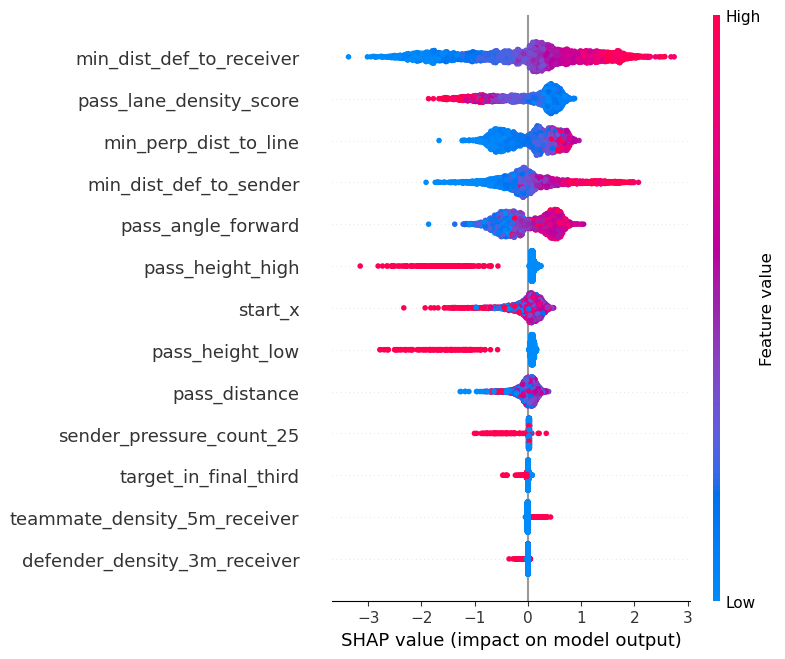
\includegraphics[width=0.85\textwidth]{images/xpass_shap.png}
    \caption{SHAP bee-swarm plot showing feature impact on the xPass model output. Positive SHAP values indicate that a feature pushes the prediction towards completion, while negative values push towards failure. Features are ordered by global importance, with the distance to the receiver (\texttt{min\_dist\_def\_to\_receiver}) and pass distance being the strongest drivers.}\label{fig:xpass-shap}
\end{figure}

\subsubsection{Calibration}\label{sec:calibration}

A scouting metric needs \emph{probabilities}, not just a good ranking: xEPV multiplies xPass by a value, so a miscalibrated $0.9$ that should be $0.7$ would directly distort every decision score.
The raw model output is passed through a sigmoid calibrator and then clipped to $[0.05,\,0.99]$:
\begin{itemize}
    \item Sigmoid calibrator (chosen over isotonic and beta). The corpus is heavily imbalanced (${\sim}90\%$ completions), so raw probabilities pile up near~1. In that saturated regime, isotonic (a flexible step function) tends to over-fit the extremes, whereas the two-parameter sigmoid fits a smooth, stable monotone correction. The choice was made on an honest 50/50 match holdout: each calibrator is fit on one half of the matches and scored on the other, so the calibrator never sees its evaluation data. On that holdout the three are near-identical on the global metrics (AUC $\approx 0.92$, Brier $\approx 0.057$ for all), so the decision is not driven by a headline-number gap; the sigmoid is preferred because it behaves the most stably across the saturated upper range, where isotonic's step function is the most fragile. Calibration is about \emph{shape}, not ranking, so a tie on AUC is expected and the tie-breaker is robustness.
    \item \textbf{Asymmetric clip $[0.05,\,0.99]$.} The lower bound protects against rare base-model saturations near~0 that would otherwise make xEPV's turnover term explode. The upper bound reflects that even the easiest decile of passes completes at ${\sim}0.997$, so anything above $0.99$ carries no tactical signal.
\end{itemize}

\subsection{xEPV: Expected Net Possession Value}\label{sec:xepv}

\textbf{xEPV} is the expected net possession value of \emph{attempting} a given pass:
\begin{equation}\label{eq:xepv}
    \text{xEPV}(t) = \text{xPass} \cdot \text{EPV}(x_t,\, y_t) \;-\; (1 - \text{xPass}) \cdot \text{EPV}(105 - x_t,\, y_t),
\end{equation}
where $\text{EPV}(x, y)$ is read from the same fixed EPV grid used in H1 (\cref{sec:epv-action}), so a location is worth exactly the same here as in the space-control study.
The first term is the \emph{reward}: the value at the target if the pass arrives.
The second term is the mirrored failure cost, and the mirroring is the key idea.
If possession is turned over at the target, the \emph{opponent} now attacks in the opposite direction; so the danger to us is the value of that point read from his side of the pitch.
On a $105$\,m-long pitch, reflecting the $x$-coordinate to $105 - x$ flips the location onto the opponent's attacking frame (the $y$-coordinate is unchanged, because only the attacking direction reverses, not the side of the pitch).
A turnover deep in the opponent's half therefore costs little (the mirrored point $105 - x$ is then near \emph{our} goal-line, a low-EPV zone for him), while a turnover in our own build-up is punished heavily.
The two terms are weighted symmetrically, 1\,:\,1 (turnover-penalty scale $= 1.0$): a turnover is treated as costing exactly what the completion would have gained, at the mirrored point.

This shape stops the metric from loving reckless ambition: a low-percentage 40-metre pass into a dangerous zone has a high reward term but a low completion probability and a heavy mirrored penalty, so its xEPV is honestly mediocre.
The robustness analysis (\cref{sec:h2-validation}) confirms that the turnover scale sets the \emph{level} of the numbers but not the ranking of players, so it is not a tuned knob hiding a result.

The xEPV definition lives in one place in the code and is imported unchanged by both H2 and H3, so the value attached to a given candidate is identical across the two studies (median difference $0.000$ on shared events).

\clearpage
% ============================================================
\section{H1: Space Control and Value}\label{sec:h1}
% ============================================================

\textbf{Hypothesis~1.}
A player's quality is measurable through his spatial influence on the pitch, not his volume.
We measure influence on three layers: the shape of the opposing block (convex hulls of the visible defenders), the threat added with each ball progression (EPV), and the pull a player exerts on the defenders around him (gravity).

\subsection{Building Blocks}\label{sec:h1-blocks}

Before the four indices, three primitives are computed on every open-play pass that has a 360 freeze frame.
The indices are aggregates of these.

\subsubsection{The Convex Hull of the Defence}\label{sec:hull}

For each pass we take the visible opponents in the freeze frame and compute their convex hull: the smallest polygon that encloses them all.
This polygon is our working model of the defensive block.
We chose the convex hull because it is the simplest object that captures the single thing a scout cares about here: \emph{``is the ball inside or outside the defensive shape, and does this action move it across the boundary?''}

A pass that ends inside the hull has entered the block; a pass that starts inside and ends outside has exited it; a touch taken inside the hull is a between-the-lines reception.
Every H1 spatial metric is, at bottom, a statement about a pass relative to this polygon.

The pitch is divided into a $12 \times 8$ grid of zones (about $8.75\,\text{m} \times 8.5\,\text{m}$ each), used to build positional baselines for the gravity computation (\cref{sec:gravity-block}).
Twelve columns by eight rows is fine enough to localise an action to a meaningful area of the pitch, coarse enough that each zone still collects enough events to form a stable baseline.

\subsubsection{EPV on Every Action}\label{sec:epv-action}

Each open-play pass is assigned an EPV value at its start and end location, read from a fixed EPV grid (a $32 \times 50$ lookup from Friends-of-Tracking-Data~\cite{epv}, values ranging from ${\sim}0.004$ in the own goal area to ${\sim}0.57$ near the opponent goal) by bilinear interpolation (so value varies smoothly across the pitch rather than jumping between grid cells).
The EPV added by a pass is the increase in scoring probability from its origin to its destination:
\begin{equation}\label{eq:epv-added}
    \text{EPV}_{\text{added}} = \text{EPV}(x_{\text{end}}, y_{\text{end}}) - \text{EPV}(x_{\text{start}}, y_{\text{start}}).
\end{equation}
This is the quantity that makes H1 contextual: a 30-metre sideways pass in front of the defence adds almost nothing, while a 10-metre pass that splits the block adds a lot.

Beyond the scalar \texttt{epv\_added}, every pass is also tagged with a geometric type based on its topology relative to the hull:
\begin{itemize}
    \item Penetration: pass starts outside the hull and ends inside it.
    \item Exit: starts inside and ends outside.
    \item Inside Circulation: starts and ends inside.
    \item Outside Circulation: starts and ends outside.
\end{itemize}
This four-way classification feeds directly into the Dangerousness radar: the four EPV-by-zone sub-components are the per-90 EPV added within each geometric type.

\subsubsection{Line-Breakers Under Three Lenses}\label{sec:linebreakers}

A ``line-breaker'' is a pass that bypasses defenders and breaks a line of the opposing block.
The obvious question is which passes count, and we deliberately refused to settle it with a single definition, because ``breaking a line'' can mean two genuinely different things: a bold geometry (splitting bodies) or a high value (creating danger). The best passes do both.
So we compute three flags:

\begin{enumerate}
    \item Geometric line-breaker: a successful pass that bypasses at least 3~opponents inside a 5-metre corridor along the pass line. The corridor width of $5$\,m was chosen because it captures defenders who are genuinely in the path of the ball (close enough to attempt an interception), while excluding those positioned laterally. The threshold of 3~opponents ensures that only passes which meaningfully disrupt the block's shape are counted; fewer than~3 would admit routine horizontal passes through a single line. This is the \emph{bold-geometry} lens: it counts passes that physically go through people, regardless of where on the pitch.
    \item Quality (EPV) line-breaker: a successful pass whose EPV added is above the role-specific 75th~percentile of positive EPV-added passes. The 75th~percentile is taken within role so that a centre-back is judged against centre-backs, not against attackers who naturally add more EPV per pass. The choice of the 75th (rather than, e.g., the median or 90th) balances selectivity (only the top quarter of value-adding passes qualify) against volume (enough passes survive to form a stable per-90 rate). This is the \emph{high-value} lens.
    \item Clean line-breaker: the intersection of the two, which is a pass that is both geometrically bold and high value.
\end{enumerate}

Reporting all three (as the Progression mother variables \texttt{LB Geom\,/\,90}, \texttt{LB Quality\,/\,90}, \texttt{LB EPV\,/\,90}) lets the index tell apart a player who breaks lines often but cheaply from one whose every line-break is dangerous.
The mean number of opponents removed per progressive pass, Def.\,Bypassed Avg, is tracked alongside as the per-pass ``boldness'' companion to the per-90 volumes.

\subsubsection{Gravity, Measured Leave-One-Out}\label{sec:gravity-block}

Gravity asks how much the defence reacts to a player.
The danger in measuring this is obvious: a player who simply plays in a crowded central zone will look ``gravitational'' just because defenders are always near the middle.
We remove that confound with a leave-one-out (LOO) baseline.

For each player, the expected defender behaviour in a given (match, zone) cell of the $12\times8$ grid is computed from everyone else's events in that same zone, excluding the player's own.
The player's gravity is then how far the defenders deviate \emph{from that baseline} when he is the one on the ball.
This turns ``defenders are near him'' into ``defenders are near him \emph{more than the zone alone explains},'' which is the only version of the claim worth scouting.

Three gravity signals come out of this baseline, and we keep them separate on purpose because they capture different pulling behaviours. They are the three values shown on the player card: \textbf{Space Attraction\,\%}, \textbf{Gravity Hull\,\%}, and \textbf{Def.\,Pull\,(m)}.

\paragraph{Space Attraction\,\% (the proximity signal).}
This uses the $K = 4$ nearest opponents. For each event we take the mean distance from the ball to the player's four closest visible defenders, $\bar d_{\text{player}}$, and compare it to the leave-one-out baseline distance for that zone, $\bar d_{\text{base}}$. The metric is the relative reduction in that distance:
\begin{equation}\label{eq:gravity-prox}
    \text{Space Attraction\,\%} = \frac{\bar d_{\text{base}} - \bar d_{\text{player}}}{\bar d_{\text{base}}} \times 100.
\end{equation}
The sign is the whole point: a player who pulls defenders toward him sits closer than the zone's baseline, so $\bar d_{\text{player}} < \bar d_{\text{base}}$ and the value is positive; a player the defence ignores sits at or beyond the baseline and scores near zero or negative.
The choice of $K = 4$ is a robustness compromise: $K = 1$ would be noisy, fluctuating whenever a single defender happens to pass nearby; $K = \text{all}$ would dilute the signal with defenders on the far side of the pitch who have nothing to do with local pressure. $K = 4$ captures the core of the local defensive cell (roughly the number of opponents who genuinely compress the space around a ball-carrier) while staying insensitive to outliers. As a safety fallback, $\min(K, |\text{visible opponents}|)$ is used, so frames with fewer than four visible defenders still contribute rather than being dropped.

\paragraph{Gravity Hull\,\% (the block-shape signal).}
This applies the same baseline-relative formula as \cref{eq:gravity-prox}, but to the area of the defensive convex hull $A$ instead of the nearest-defender distance:
\begin{equation}\label{eq:gravity-hull}
    \text{Gravity Hull\,\%} = \frac{A_{\text{base}} - A_{\text{player}}}{A_{\text{base}}} \times 100.
\end{equation}
It measures how much the whole defensive block shrinks around the player versus the zone baseline, on the same scale and with the same sign convention as Space Attraction\,\%.

\paragraph{Def.\,Pull\,(m) (the directional signal).}
The first two ask \emph{how tightly} the defence packs; this one asks \emph{in which direction} it moves. We take the opponents' centroid (their mean position) and measure how far it shifts toward the player, in metres, relative to the LOO baseline centroid. Writing $\mathbf{c}_{\text{obs}}$ for the observed centroid, $\mathbf{c}_{\text{base}}$ for the baseline centroid and $\mathbf{p}$ for the player's position:
\begin{equation}\label{eq:gravity-dir}
    \text{Def.\,Pull\,(m)} = \frac{(\mathbf{c}_{\text{obs}} - \mathbf{c}_{\text{base}}) \cdot (\mathbf{p} - \mathbf{c}_{\text{base}})}{\lVert \mathbf{p} - \mathbf{c}_{\text{base}} \rVert}.
\end{equation}
This is the projection, in metres, of the centroid's actual displacement onto the direction pointing from the baseline centroid to the player. A positive value means the defensive centre of mass genuinely slides \emph{toward} him; it is a signed displacement, not a compactness ratio, which is why it is reported in metres and kept apart from the two percentage signals.

The baseline for all three is taken at match level when there are enough frames (a minimum of 10~frames per team-zone cell, set by \texttt{MIN\_BASELINE\_FRAMES\,=\,10}) and falls back to a tournament-level baseline when a single match has too few.
This match-first-with-fallback rule is a deliberate bias/variance trade: match-level is the most relevant comparison, but only when it has the data to be stable.

\subsection{The Four Indices}\label{sec:h1-indices}

H1 produces four indices.
The single most important design decision in H1 is that \emph{three of them are treated as composites and one as a magnitude}. This is not a cosmetic label; it changes how the headline number is built:

\begin{itemize}
    \item Progression, Reception, Gravity are stylistic composites. Each models a latent style that shows up across several correlated indicators (a ``reflective'' model in measurement terms). For these, \emph{averaging the within-role percentiles} of the mother variables is the correct aggregation: no single variable is the construct, they jointly indicate it.
    \item \textbf{Dangerousness} is a magnitude. The total EPV a player creates is a real, directly measurable quantity, and it is by construction the sum of four EPV sub-components. Averaging percentiles here would be wrong, as it would throw away the fact that the parts literally add up to the whole. So the Dangerousness headline is the within-role percentile of EPV Added\,/\,90 itself, which is a single honest magnitude.
\end{itemize}

\paragraph{Handling structural NaN\,s.}
Not every mother variable is defined for every player.
A centre-back who never receives inside the opposing hull has no \texttt{pressure\_resistance\_pct}; a forward who never penetrates from outside has no \texttt{epv\_penetration\_*}.
These are structural missing values; they arise because the player's role naturally excludes certain geometric situations, not because of data error.
When a mother variable is NaN for a given player, that variable is excluded from his percentile average and the composite is computed over the remaining variables.
This is the correct treatment: imputing a value (e.g.\ zero or median) would inject false signal, while dropping the player entirely would discard a valid profile on the axes that \emph{are} observed.
One structural regularity serves as a pipeline sanity check: the fourth EPV sub-component, \texttt{epv\_outside\_circ}, has zero NaN\,s across the 272-player pool, because every outfield player in open play makes at least one pass that both starts and ends outside the opponent hull. Indeed, outside-block circulation is the universal baseline of possession football.

\subsubsection{Progression: Volume of Forward Play}\label{sec:progression}

How often, and how cleanly, a player moves the ball through opponent lines.
Five mother variables, averaged as within-role percentiles. The first three are the per-90 rates of the three line-breaker lenses defined in \cref{sec:linebreakers} (LB Geom\,/\,90 bold-geometry, LB Quality\,/\,90 high-value, LB EPV\,/\,90 their clean intersection); the last two add block-entry volume and per-pass boldness:

\begin{enumerate}
    \item Hull Penetr.\,/\,90: per-90 volume of successful passes that enter the opposing convex hull.
    \item Def.\,Bypassed Avg: mean number of opponents removed from play per progressive pass.
\end{enumerate}

Because the index blends bold-geometry volume, high-value volume, their clean intersection, block-entry volume and per-pass boldness, a player can reach the top two different ways: as a high-volume metronome (Kroos, Modric) or as a vertical specialist on lower volume whose few passes are bold and valuable (Alexander-Arnold).

\subsubsection{Dangerousness: Magnitude of EPV Creation}\label{sec:dangerousness}

The total expected possession value a player generates per 90~minutes.
The headline is the within-role percentile of EPV Added\,/\,90 alone, which is a direct magnitude rather than a composite.
The radar that decomposes it shows the four additive EPV-by-zone components (they sum to EPV Added\,/\,90 by construction):

\begin{enumerate}
    \item EPV Penetr.\,/\,90: value added on passes that enter the opposing block.
    \item EPV In-Circ\,/\,90: value circulated \emph{inside} the block.
    \item EPV Exit\,/\,90: value of clean ball-exits from inside the block back out.
    \item EPV Out-Circ\,/\,90: value circulated outside the block.
\end{enumerate}

Reading the four together explains where a player's EPV comes from, and this is the scouting payoff of decomposing rather than just totalling: a centre-back produces value mostly through Out-Circ and Penetr.; a between-the-lines attacking midfielder mostly through In-Circ and Exit; a winger drifting inside through Penetr.\ and In-Circ.

\subsubsection{Reception: Between-the-Lines Play}\label{sec:reception}

How often a player receives the ball \emph{inside} the opposing block, and how well he survives when pressed.
Three mother variables, averaged as within-role percentiles:

\begin{enumerate}
    \item Between Lines\,\%: share of touches taken inside the opponent convex hull.
    \item Hull Exits\,/\,90: per-90 volume of clean ball-exits from inside the block.
    \item Press.\,Resist\,\%: completion rate when at least 2~opponents are within 2.5\,m at the moment of release (the project-wide ``under pressure'' definition from \cref{sec:conventions}).
\end{enumerate}

This index deliberately measures \emph{where you stand}, not how many touches you take, which is why it surfaces Pedri, Wirtz, and a cluster of ball-playing centre-backs (Calafiori, Matvienko, Krej\v{c}\'{\i}). These players are valuable because they make themselves available between the lines, which is something volume statistics cannot capture.

\subsubsection{Gravity: Spatial Pull on the Defence}\label{sec:gravity}

How much the opposing defenders move \emph{because of you}, measured leave-one-out (\cref{sec:gravity-block}).
Three mother variables, averaged as within-role percentiles, the same three shown on the player card:

\begin{enumerate}
    \item \textbf{Space Attraction\,\%}: how much \emph{closer} the four nearest defenders sit than the zone's leave-one-out baseline (\cref{eq:gravity-prox}).
    \item \textbf{Gravity Hull\,\%}: the same baseline-relative measure applied to the area of the defensive block (\cref{eq:gravity-hull}).
    \item \textbf{Def.\,Pull\,(m)}: the signed displacement, in metres, of the opposing defensive centroid toward the player (\cref{eq:gravity-dir}).
\end{enumerate}

Gravity is, by deliberate design, the one index where internal consistency is \emph{negative} (see \cref{sec:h1-validation}).
This is not a defect; it is the honest consequence of the construct.
A forward who drags a centre-back out wide and a winger who pins both full-backs inside are both ``gravitational,'' but they are doing different things, so their mother variables do not move together.
Gravity measures the \emph{union} of these pulling behaviours, not a single coherent skill, and we report it as such.

\subsection{Validation}\label{sec:h1-validation}

\subsubsection{Internal Consistency (Cronbach's $\alpha$)}\label{sec:cronbach}

Cronbach's~$\alpha$ asks whether the mother variables of a composite move together (whether they measure ``one thing'').
We report it per index in \cref{tab:alpha}, but crucially we interpret it differently depending on what the index is meant to be.

\begin{table}[H]
\centering
\caption{Internal consistency (Cronbach's $\alpha$, averaged over the 6 roles).}\label{tab:alpha}
\small
\begin{tabularx}{\textwidth}{@{}lrL@{}}
\toprule
Index & Mean $\alpha$ & Interpretation \\
\midrule
Progression & 0.77 & Tight construct, where the 5 variables genuinely measure one dimension. \\ \midrule
Dangerousness & 0.32 & Diagnostic only; the four radar axes are additive EPV components, not a reflective composite. Low $\alpha$ is expected, not a problem. \\ \midrule
Reception & 0.41 & Moderate composite, scoring high on CB and CAM, lower on FW due to small sample. \\ \midrule
Gravity & $\boldsymbol{-0.03}$ & Multi-directional by design, since the three variables capture different pulling phenomena (see \cref{sec:gravity}). \\
\bottomrule
\end{tabularx}
\end{table}

The four indices are also only weakly correlated with each other (absolute correlation at most $0.56$ across the full pool, against a target below $0.6$), meaning there is no redundancy. Each index carries its own signal, and the four-card profile does not present four views of the same number.

\paragraph{A notable cross-index finding.}
The variable redundancy analysis revealed one strong and substantively interesting correlation between variables that live in \emph{different} index families: \texttt{between\_lines\_pct} (a Reception variable) and \texttt{gravity\_proximity\_pct} (a Gravity variable) correlate at $\rho \approx 0.91$.  This says that players who frequently receive between the opposing lines are also the ones who, on average, draw the nearest defenders closest to them when they have the ball.  The finding is genuine rather than a redundancy to resolve; being a ``between-the-lines receiver'' and being a ``magnet for nearby defenders'' are empirically the same player profile in this dataset. This finding strengthens the reading of both indices rather than threatening either.

\subsubsection{Contextual vs.\ Naive Rankings}\label{sec:ctx-vs-naive}

This is the experiment that tests H1's core claim, which is that ball volume is a poor proxy for value created.
For each index we take a naive volume proxy and measure how far the ranking moves when we switch to the contextual index (\cref{tab:ctx-naive}).

\begin{table}[H]
\centering
\caption{Contextual vs.\ naive (within-role, $n=272$).}\label{tab:ctx-naive}
\small
\begin{tabularx}{\textwidth}{@{}lLrrr@{}}
\toprule
Index & Naive proxy & Spearman $\rho$ & Mean $|\Delta|$ & \% $|\Delta| > 20$ \\
\midrule
Progression & passes\,/\,90 & 0.47 & 21.7 & 47\% \\ \midrule
Dangerousness & passes\,/\,90 & 0.28 & 27.8 & 54\% \\ \midrule
Reception & between-lines\,\% & 0.75 & 14.9 & 29\% \\ \midrule
Gravity & gravity proximity\,\% & 0.60 & 18.5 & 39\% \\
\bottomrule
\end{tabularx}
\end{table}

\textbf{Dangerousness} is where the gap hits hardest: more than one player in two shifts by more than 20~percentile points moving from the naive ranking (ball volume) to the contextual one (EPV magnitude).
The correlation of just $0.28$ means volume and value barely agree on who is dangerous.

\paragraph{Honesty on proxy choice.}
Progression and Dangerousness are tested against \emph{pure external volume} (passes\,/\,90), a stat that is not part of the index. This makes the test a clean ``volume versus context'' comparison.
We deliberately did not use EPV\,/\,90 as the Dangerousness proxy, because the index headline is the percentile of EPV\,/\,90, and comparing it to itself would be tautological.
Reception and Gravity are tested against one of their own raw mother variables (between-lines\,\%, gravity proximity\,\%): here the question is not ``volume vs.\ context'' but ``does the single most intuitive component reproduce the full index, or do the other components re-order it?''

\subsection{Key Findings}\label{sec:h1-findings}

A scout-first read of the Euro~2024 leaderboards, read within-role with the 135-minute floor.

\paragraph{Progression.}
Trent Alexander-Arnold (England, MID, $n=135'$) tops the index at the 95th~percentile on the smallest sample of the leaders. He plays a hybrid inverted role, showing high LB EPV volume and high Def.\,Bypassed Avg even in limited playing time.
Toni Kroos (Germany, MID) at the 93rd~percentile on 485~minutes is the metronome route.
Luka Modri\'{c} (Croatia, MID) sits at the 94th percentile and Mateo Kova\v{c}i\'{c} (Croatia, MID) at the 92nd. The Croatian double pivot reads as a strong progression duo, whereas a naive view tends to credit only Modri\'{c}.
Ball-playing centre-backs Alessandro Bastoni (Italy, CB) and Joachim Andersen (Denmark, CB) sit at 94th and 92nd among CBs, with LB EPV\,/\,90 comparable to central midfielders.
Bruno Fernandes (Portugal, MID, $n=379$) is at the 90th percentile. He is at the top of the MID pool on the line-breaking volume axes (both above the 98th~percentile), but is held to the 90th percentile overall because a smaller share of his line-breakers actually land \emph{inside} the opposing block. This is the three-lens design paying off, showing that while he breaks lines often, fewer of those breaks are ``clean'' and therefore the index ranks him high but not at the absolute top.

\paragraph{Dangerousness.}
This is where the contextual approach moves the leaderboard most: the naive-to-contextual disagreement exceeds 20~points on 54\% of the pool, the largest of all four indices.
Arda G\"{u}ler (Turkey, FW, $n=369$), Bruno Fernandes (Portugal, MID, $n=379$), Antonio R\"{u}diger (Germany, CB, $n=488$) and Joachim Andersen (Denmark, CB) all sit at 98--100 inside their role.
R\"{u}diger and Andersen sit at the top of the CB pool on EPV\,/\,90 \emph{and} on raw passing volume. While a naive view partially surfaces this, the radar (Out-Circ at 100, Penetr.\ at 84) clarifies that they are not just high-volume distributors, but are actively penetrating from the back.
The decomposition is what turns ``good passer'' into ``value-from-the-build-up-and-into-the-block.``
Tom\'{a}\v{s} Sou\v{c}ek (Czech Republic, MID, $+80$ shift), Heorhii Tsitaishvili (Ukraine, FB, $+75$) and Ivan Peri\v{s}i\'{c} (Croatia, FB, $+74$) are the largest naive-to-contextual shifts in the pool.
Sou\v{c}ek is the headline: he is in the 3rd percentile by passes\,/\,90 among MIDs but in the 83rd percentile by EPV\,/\,90. He has almost no passing volume, yet every involvement moves the value needle (his radar peaks on Exit at 100 and In-Circ at 72, which is typical of a box-arriving holding midfielder who breaks out of pressed phases). This single player is the clearest proof of the whole H1 thesis.
The mirror case is Phil Foden (England, WIDE) at the 11th (bottom of the WIDE pool): 89th~percentile of WIDE players on passes\,/\,90, but 11th on EPV Added\,/\,90.
Heavily involved in possession; his involvement just adds little expected value in this sample. Volume says star, value says otherwise.
Leroy San\'{e} (Germany, WIDE, $n=211'$) is a different case: unlike Foden he is not over-involved, since his passing volume is only mid-pool, but he scores low on every contextual axis at once, the 8th percentile of wingers on Dangerousness and the 19th on Decision Quality. He is a big name who did not make an impact in this sample.

\paragraph{Reception.}
Pedri (Spain, CAM, $n=185'$) is at the 98th percentile, emerging as the clearest between-the-lines CAM of the tournament with the highest Between Lines\,\% of any CAM and very strong Press.\,Resist\,\%.
Florian Wirtz (Germany, WIDE) sits at the 90th percentile, which is the highest in the WIDE pool. Wide attackers usually score low here because they receive on the touchline; Wirtz is the exception because he comes inside.
A cluster of ball-playing centre-backs at 88--93 inside the CB pool (Riccardo Calafiori, Mykola Matvienko, Ladislav Krej\v{c}\'{\i}, Willi Orban, Nacho Fern\'{a}ndez) surfaces cleanly thanks to the within-role lens. With the CB role-median at ${\sim}4\%$, a CB at the 90th here is genuinely the kind who steps into the half-space to receive.
Breel Embolo (Switzerland, FW) is at the 89th percentile. He is a centre-forward whose between-the-lines reception rate beats most CAMs, representing the modern ``drop-nine'' profile.

\paragraph{Gravity.}
Gravity does not depend on how much a player touches the ball, but only on how the opposing defenders react to them.
The top is therefore dominated by players from smaller national sides built around one attacking reference, which is itself a validation: the metric finds the player a defence was set up to stop.
Jan Mlakar (Slovenia, WIDE) sits at the 95th percentile. He is the index leader and ranks at the 100th percentile of WIDE players on Space Attraction\,\%.
Giorgi Kochorashvili (Georgia, MID) is at the 93rd percentile, Luk\'{a}\v{s} Provod (Czech Republic, MID) at the 92nd, and Salih \"{O}zcan (Turkey, MID) at the 92nd. These are three midfielders from sides that funnel possession through a single central player.
David Strelec (Slovakia, FW) is at the 92nd percentile. He is the only FW at the top and has the largest \emph{directional} pull of this group: the opposing defensive centroid shifts about 12\,m toward him on average, which is the highest signed displacement here. This is the directional-gravity component doing exactly what it was built for.
Kenan Y\i{}ld\i{}z (Turkey, WIDE) sits at the 84th percentile, representing a more recognisable name in the group.

A separate read on a famous name shows the value of the four-index profile. Joshua Kimmich (Germany, FB) lands at 83rd Progression, 96th Dangerousness, 72nd Reception, and 57th Gravity. This confirms the public reading on the offensive side but suggests his gravitational pull is only mid-pool inside the FB role, which is something a single number would not reveal.
\Cref{fig:h1-radar} shows his card: the four panels, one per index, are the website's H1 view, and each panel decomposes the headline percentile into its mother variables.

\begin{figure}[H]
    \centering
    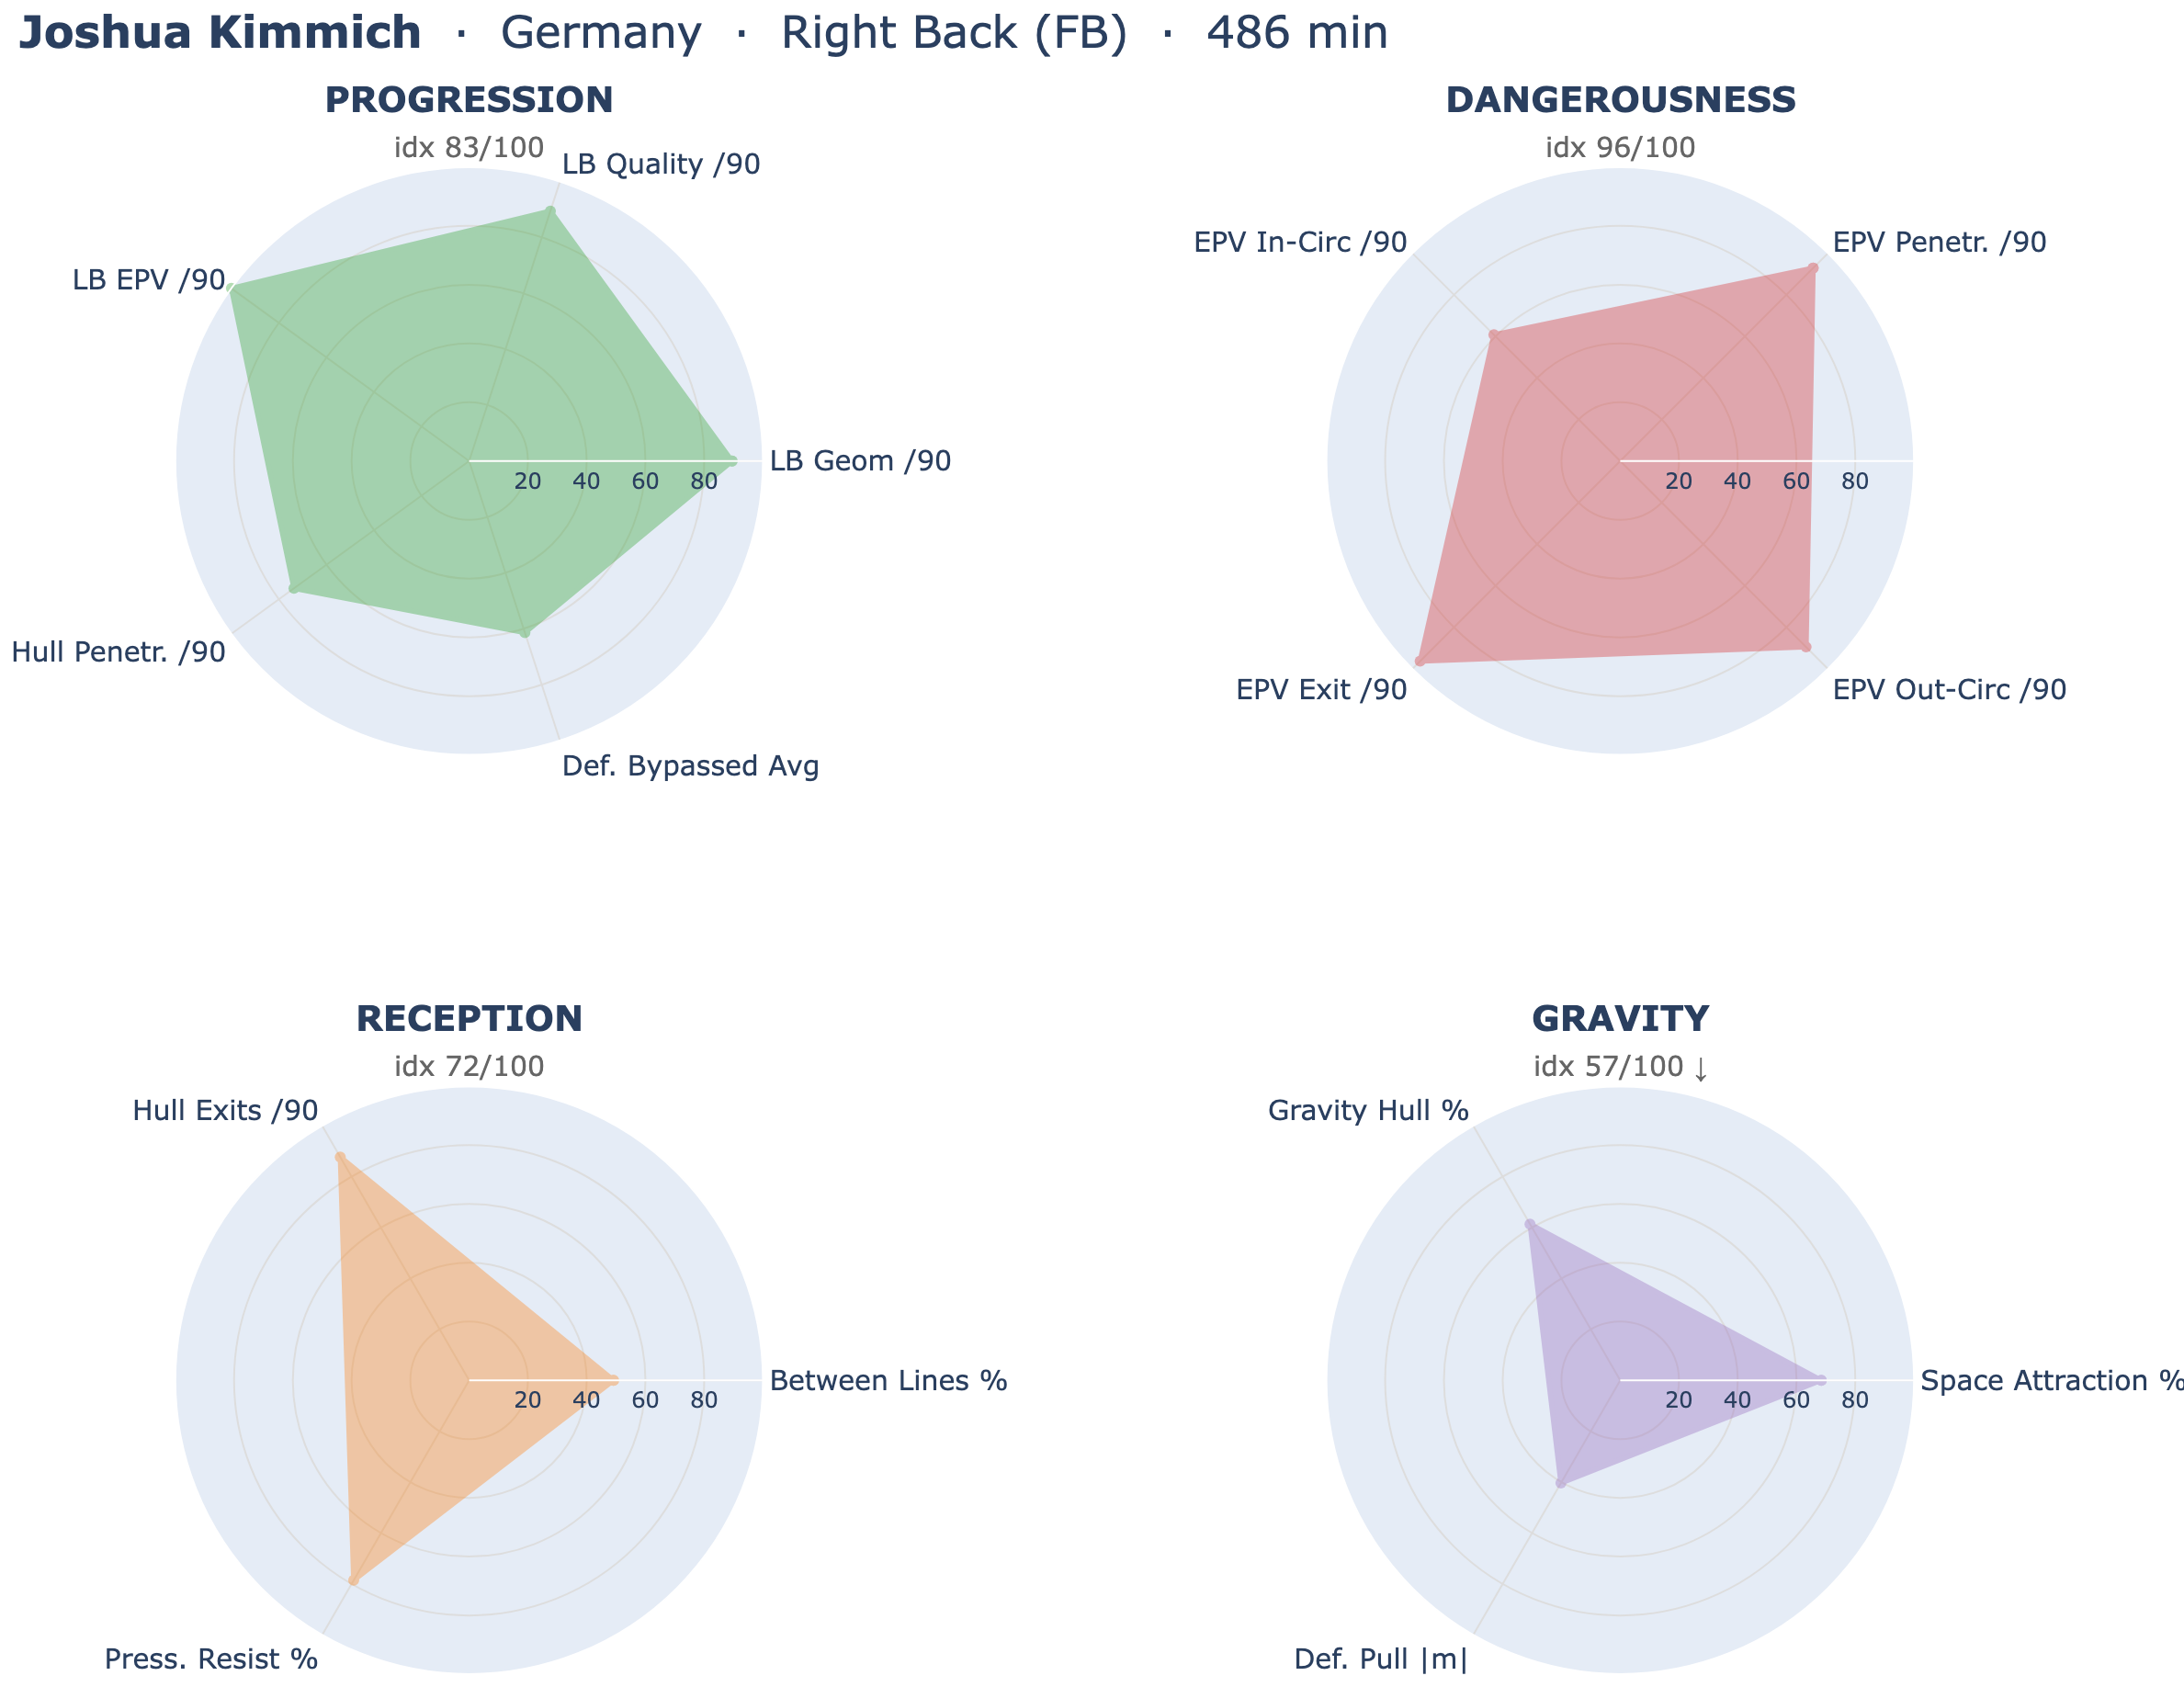
\includegraphics[width=0.9\textwidth]{images/h1_radar_kimmich.png}
    \caption{The H1 four-index card for Joshua Kimmich (Germany, FB), one panel per index. Each panel is a within-role percentile radar over that index's mother variables, and the headline percentile sits in the panel title (Progression 83, Dangerousness 96, Reception 72, Gravity 57). Read together the four panels make the point a single rating cannot: Kimmich is elite going forward but only mid-pool on the gravitational pull he exerts inside the full-back role.}\label{fig:h1-radar}
\end{figure}

\paragraph{Scouting discoveries: three faces of the test.}
The disagreement the table measures has names, and each is the top bar of its panel in \cref{fig:scouting-discoveries,fig:naive-overrating}.
Bendeg\'{u}z Bolla (Hungary, FB) is the textbook discovery: he is only in the 7th percentile of full-backs by raw volume (passes\,/\,90) yet shows the largest Progression gain in the pool ($\Delta = +65.6$~percentile points, rising to the 73rd percentile of full-backs) because the few passes he plays are clean line-breakers.
As shown in \cref{fig:bolla-linebreaker}, Bolla's line-breaking ability is not a theoretical abstraction but a concrete on-pitch reality: in this freeze-frame, he plays a diagonal pass bypassing three defenders to penetrate the opposing defensive block's convex hull.
Despite being a full-back, who typically plays in less advanced areas, this single action adds an expected possession value of $0.0766$ ($\text{EPV}+$), which is more than twelve times the role-specific 75th percentile threshold of $0.0061$ for a quality line-breaker.
This visualises exactly how the Progression index filters out the volume bias and highlights high-value, space-disrupting involvements.

\begin{figure}[H]
    \centering
    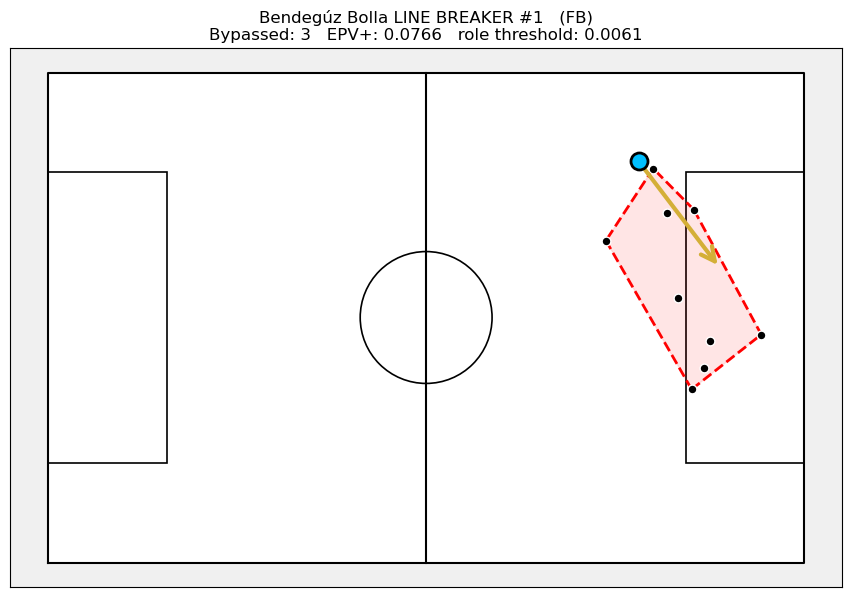
\includegraphics[width=0.92\textwidth]{images/linebreaking_pass_1.png}
    \caption{Visualisation of a clean line-breaking pass by Bendeg\'{u}z Bolla (Hungary, FB) during Euro 2024. Bolla (blue circle at the top-right) plays a diagonal pass that bypasses three opponents inside the opposing defensive block's convex hull (shaded red region). The pass generates an EPV added of $0.0766$, far exceeding the Full-Back role-specific threshold of $0.0061$ for quality line-breakers.}\label{fig:bolla-linebreaker}
\end{figure}

Tom\'{a}\v{s} Sou\v{c}ek (Czech Republic, MID) shows the same phenomenon on threat rather than progression: he is in the 3rd percentile of midfielders by passes\,/\,90 but the 83rd by EPV created, representing one of the largest Dangerousness gains in the pool ($\Delta = +80$). He has almost no passing volume, yet every involvement moves the value needle.
The mirror keeps the test honest: Phil Foden (England, WIDE) is the most naive-overrated player on Dangerousness ($\Delta = -78$), sitting in the 89th percentile by passes\,/\,90 but only the 11th by EPV created, meaning he is heavily involved yet adds little expected value.
Two players the volume ranking buries and one it inflates: exactly the re-ordering the Spearman correlations quantify.

\begin{figure}[H]
    \centering
    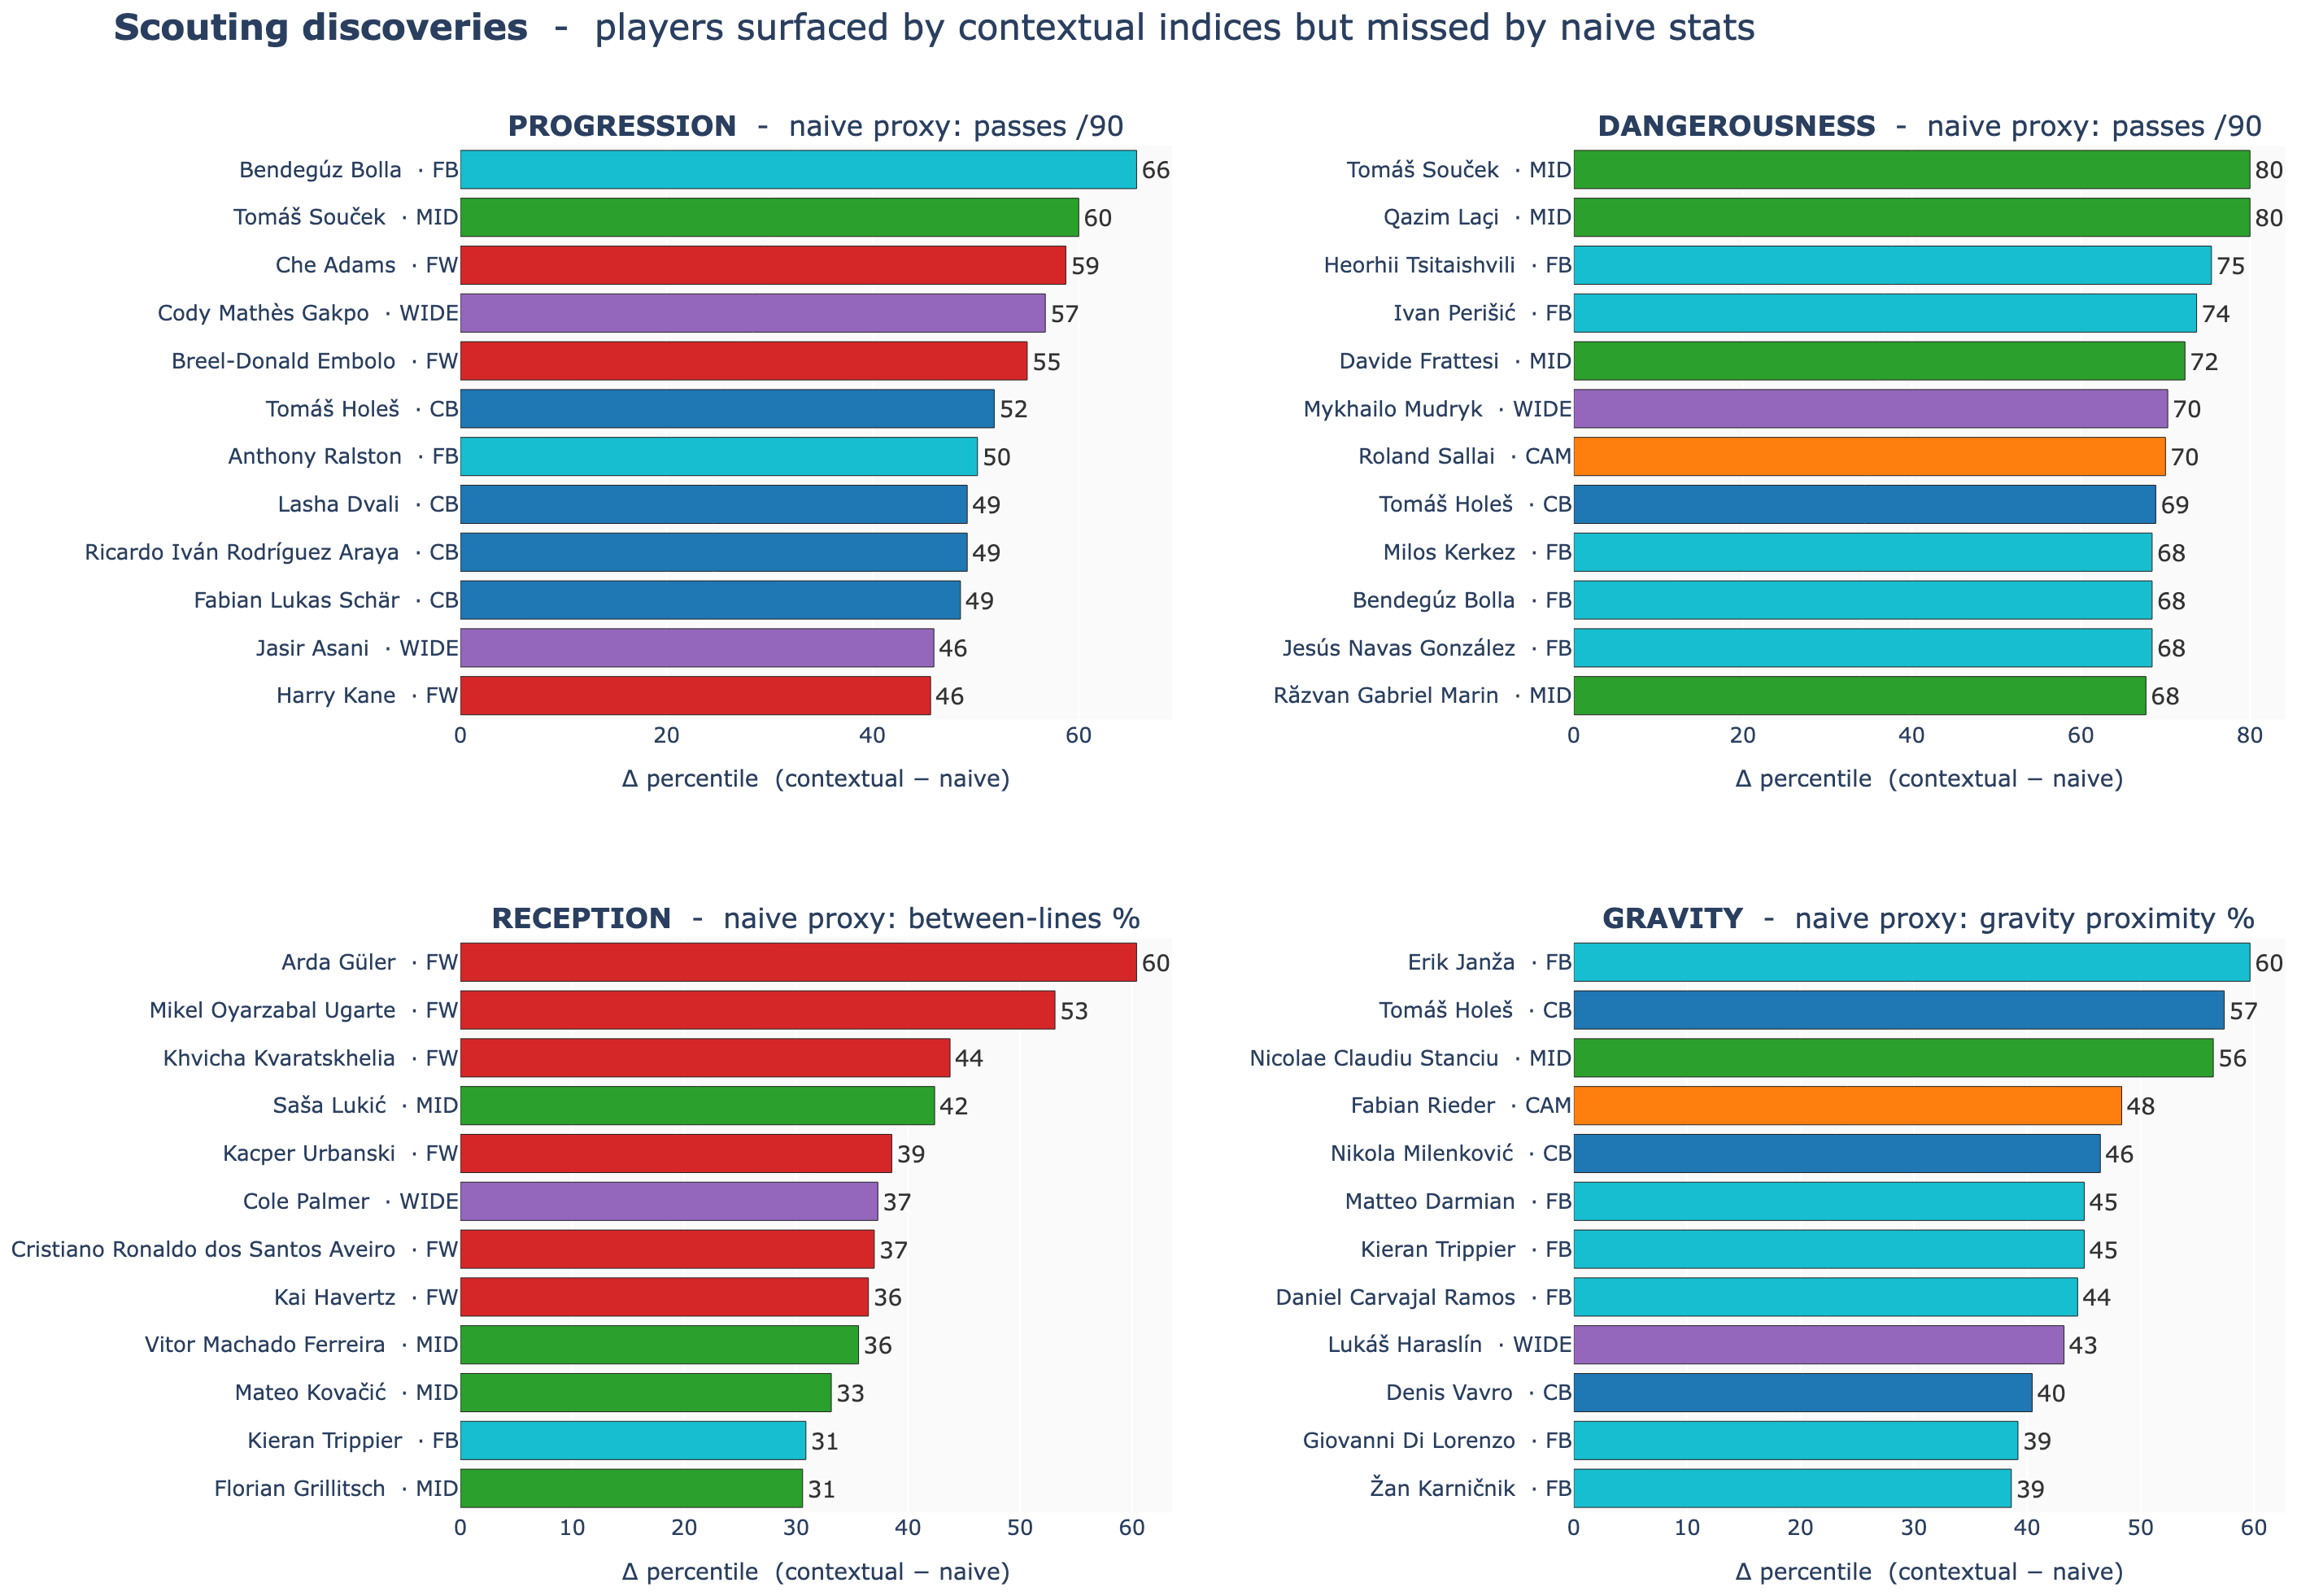
\includegraphics[width=\textwidth,height=0.6\textheight,keepaspectratio]{images/scouting_discoveries.png}
    \caption{Scouting discoveries and naive overrating (see also \cref{fig:naive-overrating}). One panel per index. Each bar is a player's $\Delta$~percentile $=$ contextual index $-$ naive proxy, computed within his macro-role and coloured by role; the naive proxy is passes\,/\,90 for Progression and Dangerousness, between-lines\,\% for Reception, and gravity-proximity\,\% for Gravity. The discoveries figure shows the twelve largest positive~$\Delta$ per index, representing players a naive ranking buries but the contextual index lifts (Bolla heads Progression at $+66$, Sou\v{c}ek Dangerousness at $+80$, and G\"{u}ler Reception at $+60$).}\label{fig:scouting-discoveries}
\end{figure}

\begin{figure}[H]
    \centering
    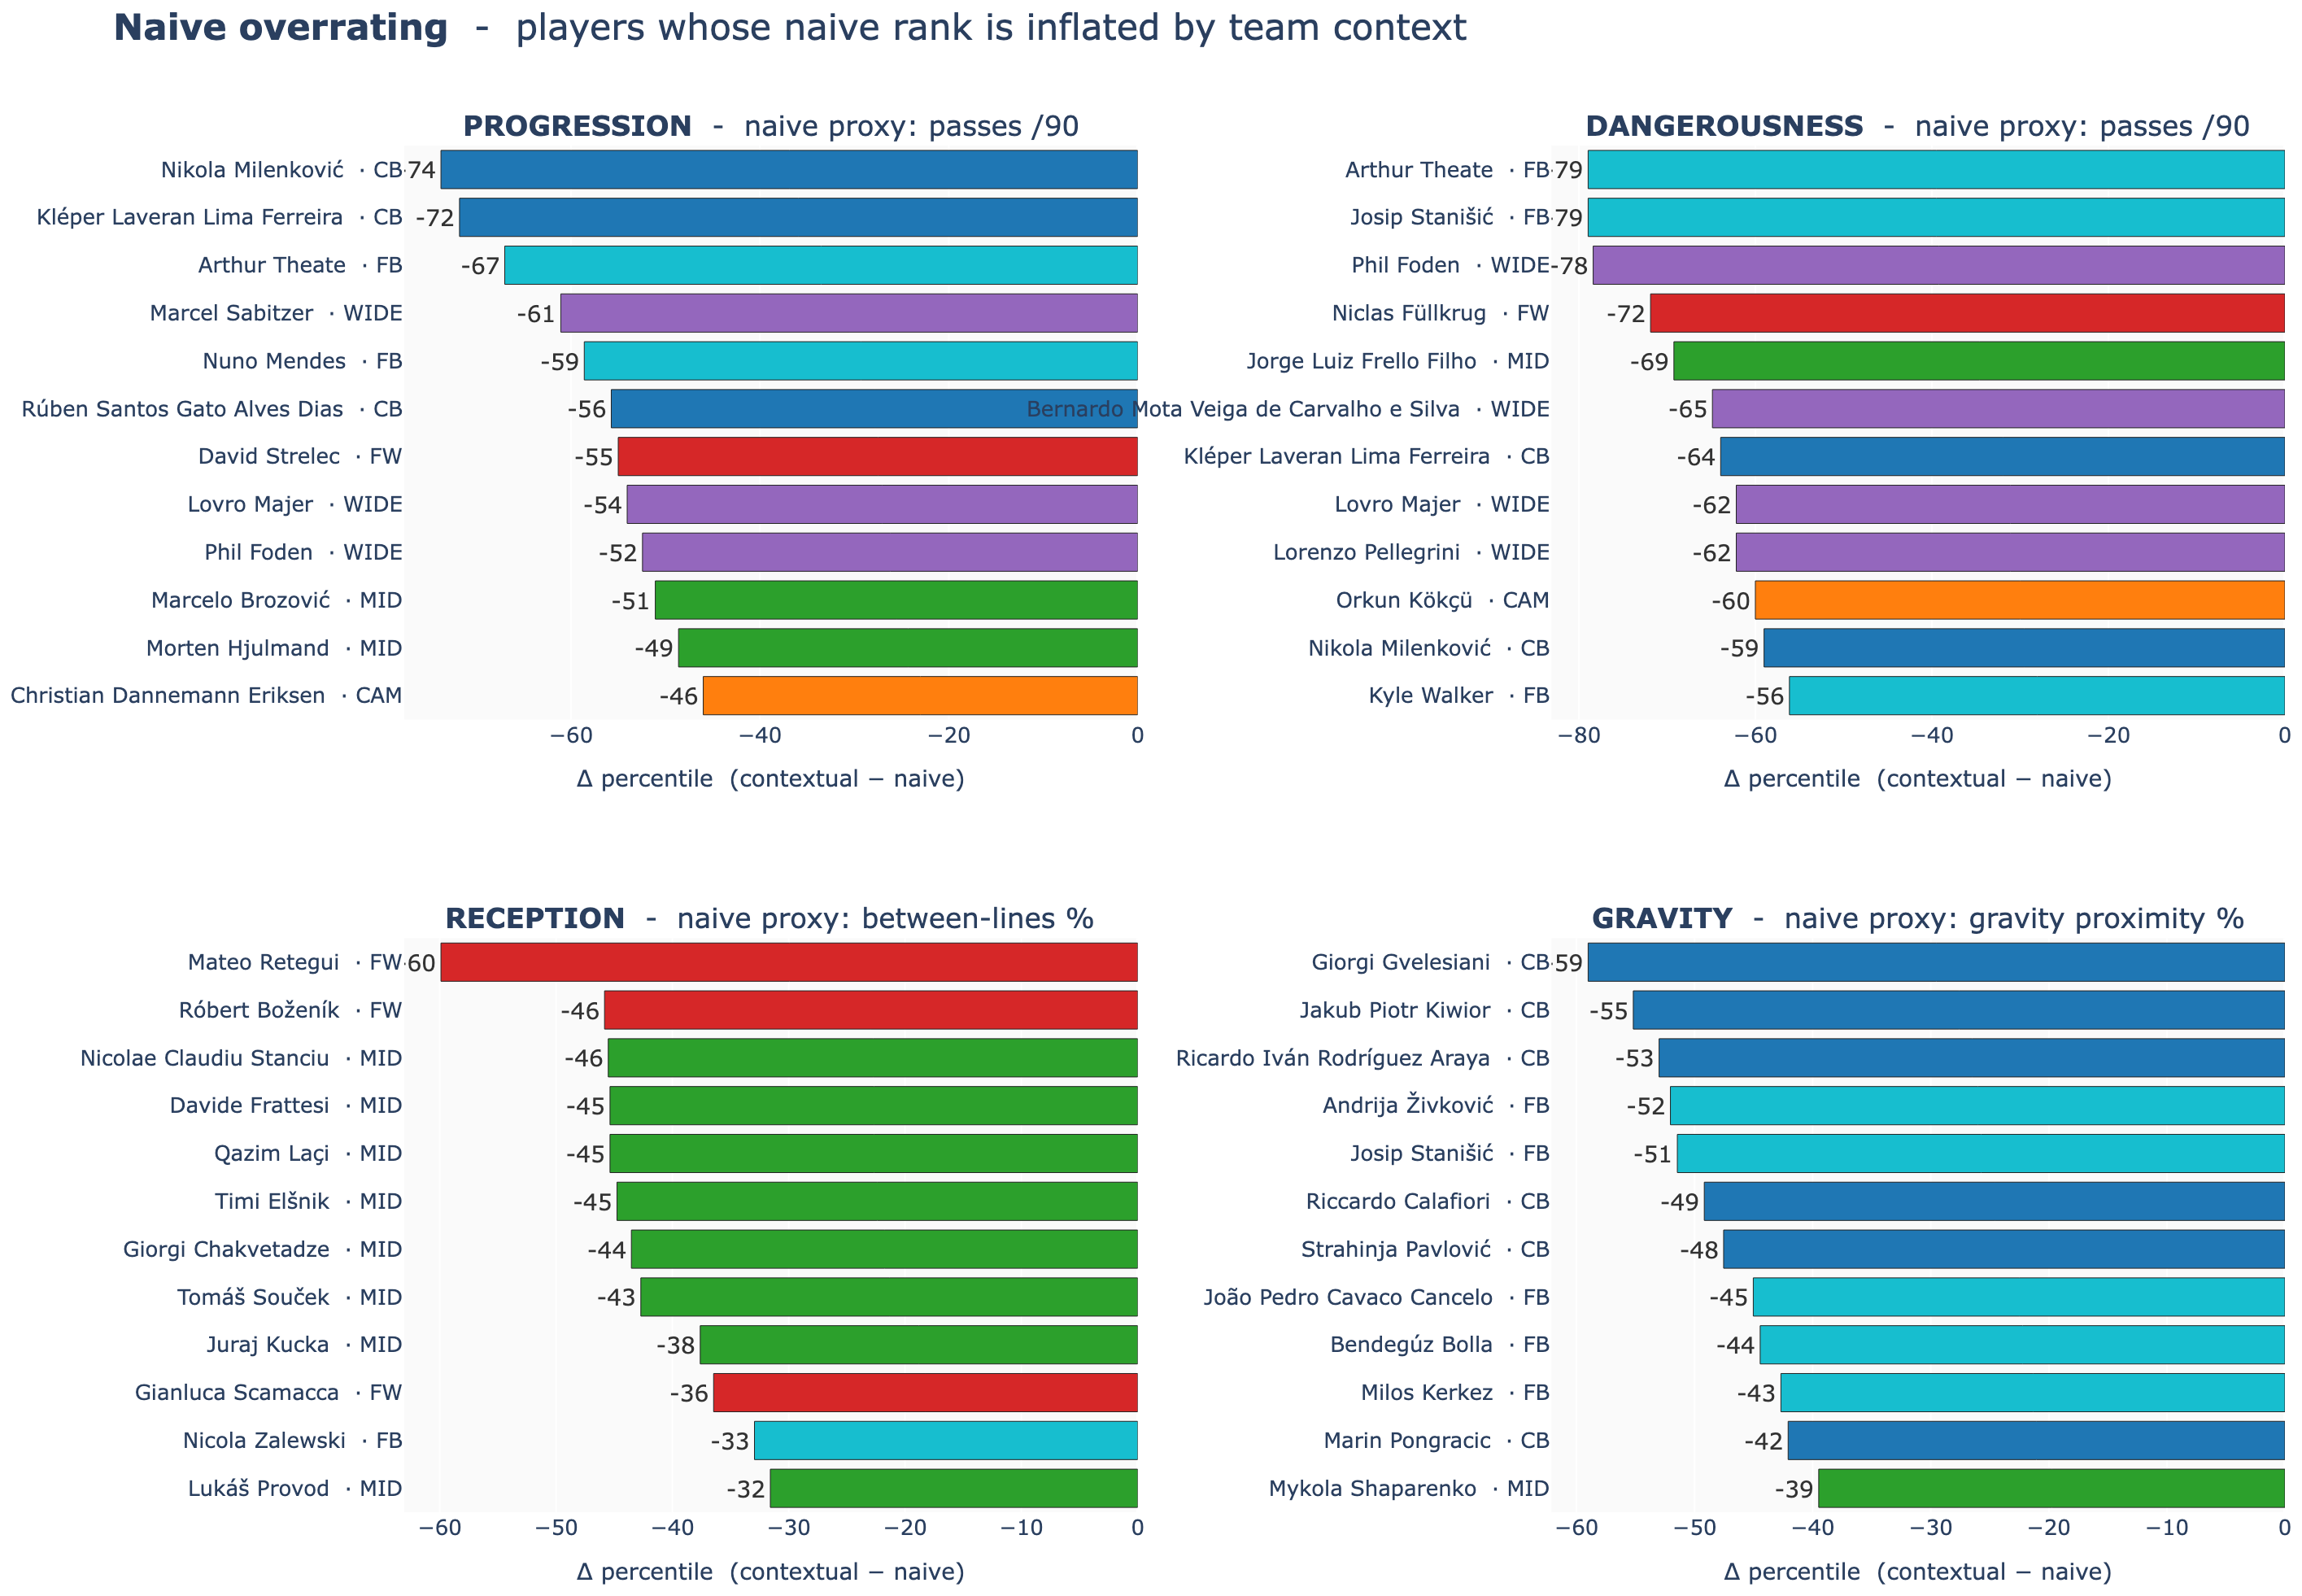
\includegraphics[width=0.95\textwidth]{images/naive_overrating.png}
    \caption{Naive overrating: the mirror of \cref{fig:scouting-discoveries}. The twelve largest negative~$\Delta$ per index, showing players whose naive (volume-based) rank is inflated by team context but whose contextual contribution is lower (such as Foden at $-78$ on Dangerousness). Together the two figures represent the visual form of the \cref{sec:ctx-vs-naive} headline test: the table shows how many players move and by how much, while the figures specify which players and in which direction.}\label{fig:naive-overrating}
\end{figure}

\clearpage
% ============================================================
\section{H2: Decision Quality}\label{sec:h2}
% ============================================================

H1 grades the value a player creates with the ball, but it says nothing about \emph{choice}: a pass can add value and still be the wrong decision, if a better option was open and ignored. H2 adds that missing layer.

\textbf{Hypothesis~2.}
A player's quality is measurable through \emph{how well he chooses} among the passing options actually available to him, which is evaluated not by the absolute value of the pass he played, but by its value relative to the options he ignored.

\subsection{Building the Choice Set}\label{sec:choice-set}

For every open-play pass we reconstruct the alternative set: every in-frame teammate the player could have passed to.
Each teammate is scored with the shared machinery (xPass, then xEPV) as if the sender had attempted that pass.
This produces, per real pass, a small menu of scored options, comprising the chosen one plus the ones ignored.

Three filtering choices shape this corpus, all deliberate:
\begin{itemize}
    \item Headed passes are excluded: passes played with the head (\texttt{body\_part\,=\,'Head'}) are removed because headers have a fundamentally different geometry and decision logic from foot passes. The sender's control over direction, height and weight is far more constrained, so grading the ``choice'' on the same feature set would be misleading.
    \item Pass-into-space is excluded: events where no in-frame teammate is within 12\,m of the chosen pass's end location. The 12\,m threshold is not arbitrary: it is about the furthest a receiver can travel during ${\sim}1.5$\,s of ball flight at sprint speed (${\sim}8$\,m/s), so it keeps genuine medium-long passes to a moving receiver while dropping true into-space balls that have no well-defined ``who did he choose.''
    \item Goalkeeper senders are excluded: a keeper's distribution (long goal kicks, unpressured box passing) has a completely different geometry from an outfield decision.
\end{itemize}

\paragraph{Height of a hypothetical pass.}
For a candidate teammate we do not know what height the sender would have used, but xPass needs it.
Forcing ``ground'' on every candidate would wrongly inflate the completion probability of long forward options nobody would ever try along the ground.
We resolved this with a single empirically-grounded rule: candidates under 30\,m are scored as ground passes, candidates over 30\,m as lofted. This is because in the real corpus passes flip from ${\sim}77$--$93\%$ ground below 30\,m to predominantly high above it ($9\%$ ground / $91\%$ high beyond 40\,m).
One distance threshold captures that regime change cleanly without per-distance tuning.

This step produces the alternatives table: 222,274 candidate rows across the corpus, about 7.2 options per event.

\subsection{The DQ Index}\label{sec:dq-index}

The headline is the \textbf{DQ index}, a relative choice-optimality index within a constrained action set.
It is built in two steps:

\begin{enumerate}
    \item \textbf{Per event.} The Score is the share of the in-frame alternatives whose xEPV is at or below the xEPV of the pass the player actually chose (restricted to events with at least 2 alternatives):
    \begin{equation}\label{eq:dq-score}
        \text{Score}_e = \frac{|\{a \in A_e : \text{xEPV}(a) \leq \text{xEPV}(\text{chosen}_e)\}|}{|A_e|}.
    \end{equation}
    \item \textbf{Per player.} The player's mean Score across all his decision events.
    \item \textbf{DQ index} = the within-macro-role percentile of that mean Score.
\end{enumerate}

What the index measures, stated precisely: it grades the chosen pass against the menu of options the frame actually offered, not against an absolute notion of the perfect pass.
It is context-normalised by construction: the comparison lives inside each event, so the pitch-zone value level cancels. Furthermore, it is bounded and interpretable on a single scale.

That there is real signal to grade is an empirical fact, not an assumption: across the events with at least two alternatives, the chosen pass is the single highest-xEPV option only 15.2\% of the time, so players take the value-optimal in-frame pass barely one time in seven. If they always picked the optimum the index would be flat and useless; the spread of how \emph{often} a player chooses near the top of his available menu is exactly what the Score, and the DQ percentile built on it, capture.

\paragraph{Why a within-event rank, and not the obvious alternatives.}
\begin{itemize}
    \item \emph{Not absolute xEPV.} Simply averaging the value of a player's chosen passes would reward players who operate in high-value zones of the pitch regardless of whether they chose well (a CAM near the box would beat a CB by position alone).
    \item \emph{Not regret-versus-best.} A ``regret'' score (how far each chosen pass falls below the single best option available) was tested and rejected, because it punishes players who consistently operate in frames where \emph{many} options are valuable.
    \item \emph{The within-event rank.} It asks the right question: \emph{given what was actually on offer in this frame, how good was the pick?}
\end{itemize}

Companion metric: Value Impact $= \text{mean}(\text{xEPV}_{\text{chosen}} - \overline{\text{xEPV}}_{\text{alternatives}})$, the value-weighted view of the same signal.
As plotted in \cref{fig:dq-vs-value-impact}, Value Impact correlates with the DQ index at Spearman $\rho \approx 0.76$ within role, confirming they capture a highly aligned tactical signal while retaining role-specific characteristics. Value Impact acts as the value-weighted companion that plays the role \texttt{epv\_added\,/\,90} plays next to the Dangerousness percentile in H1.

\begin{figure}[H]
    \centering
    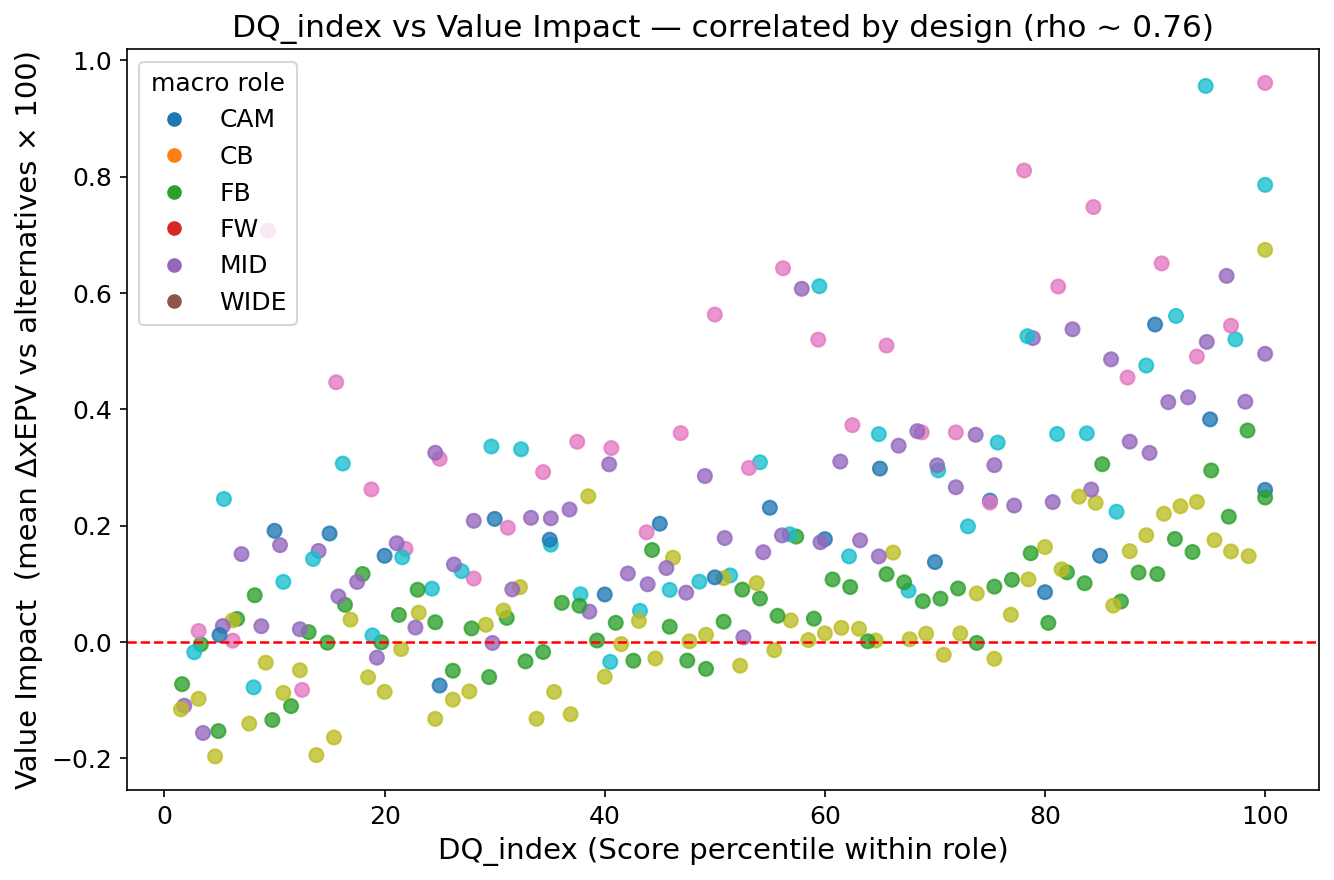
\includegraphics[width=0.9\textwidth]{images/dq_vs_value_impact.png}
    \caption{Scatter plot of DQ Index (within-role percentile) against Value Impact (mean net value added vs.\ alternatives) grouped and coloured by macro role. The two metrics are strongly correlated ($\rho \approx 0.76$) by construction, showing that high relative choice accuracy translates directly to higher quantitative expected possession value.}\label{fig:dq-vs-value-impact}
\end{figure}

\subsection{Worked Example}\label{sec:dq-example}

The same Kroos event (Germany vs.\ Scotland, minute~16) is shown twice: first, the eight in-frame candidates coloured by \textbf{xPass}; then the same eight coloured by \textbf{xEPV}, showing how the ranking changes.
A medium-probability candidate in an advanced zone can beat a near-certain pass in a low-value zone, because xEPV multiplies probability by destination value and subtracts the mirrored failure cost.
In this frame Kroos picks the candidate with chosen xPass $= 0.68$ (ranked 4th of 8 on completion probability), which carries xEPV $= +0.63$ (ranked 4th of 8 on value).
The best alternative on xEPV is at $+1.26$, a more vertical option Kroos did not take.

\begin{figure}[H]
    \centering
    \begin{subfigure}[t]{0.49\textwidth}
        \centering
        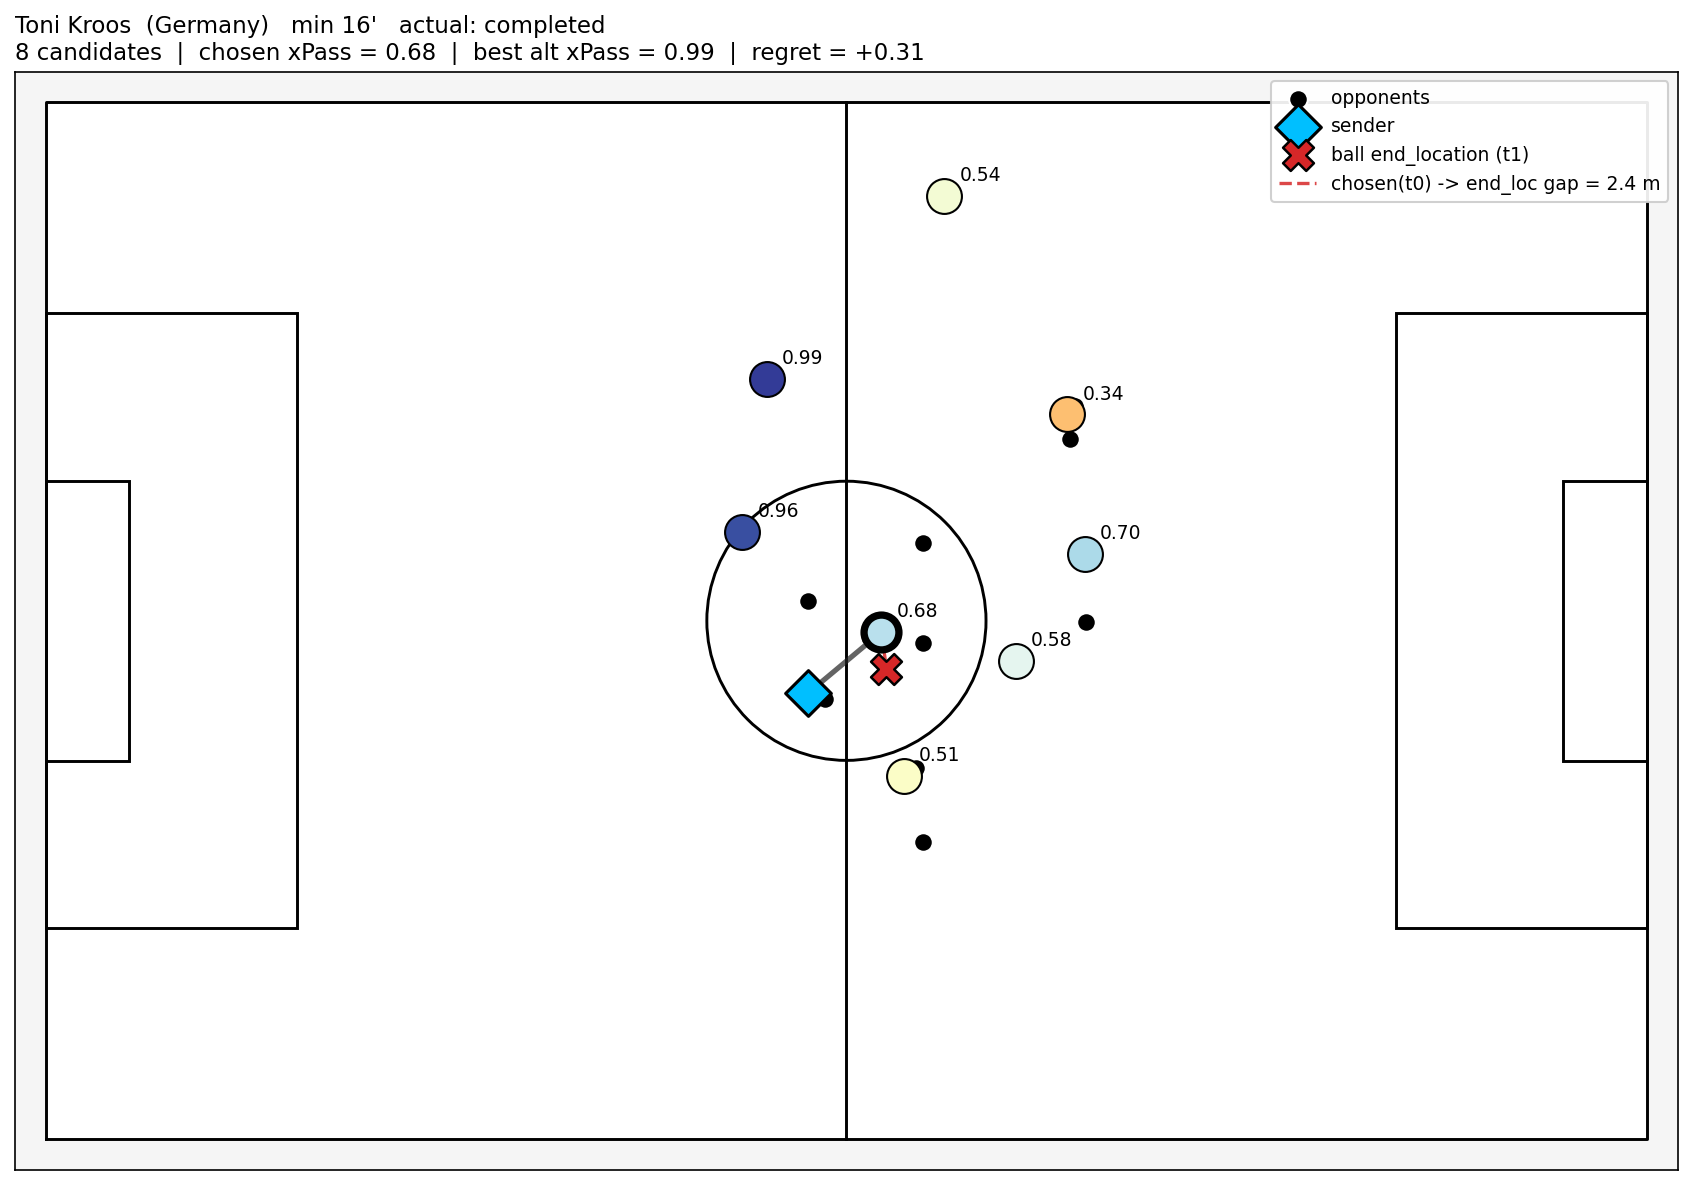
\includegraphics[width=\textwidth]{images/xpass_example.png}
        \caption{Candidates coloured by xPass.}
    \end{subfigure}
    \hfill
    \begin{subfigure}[t]{0.49\textwidth}
        \centering
        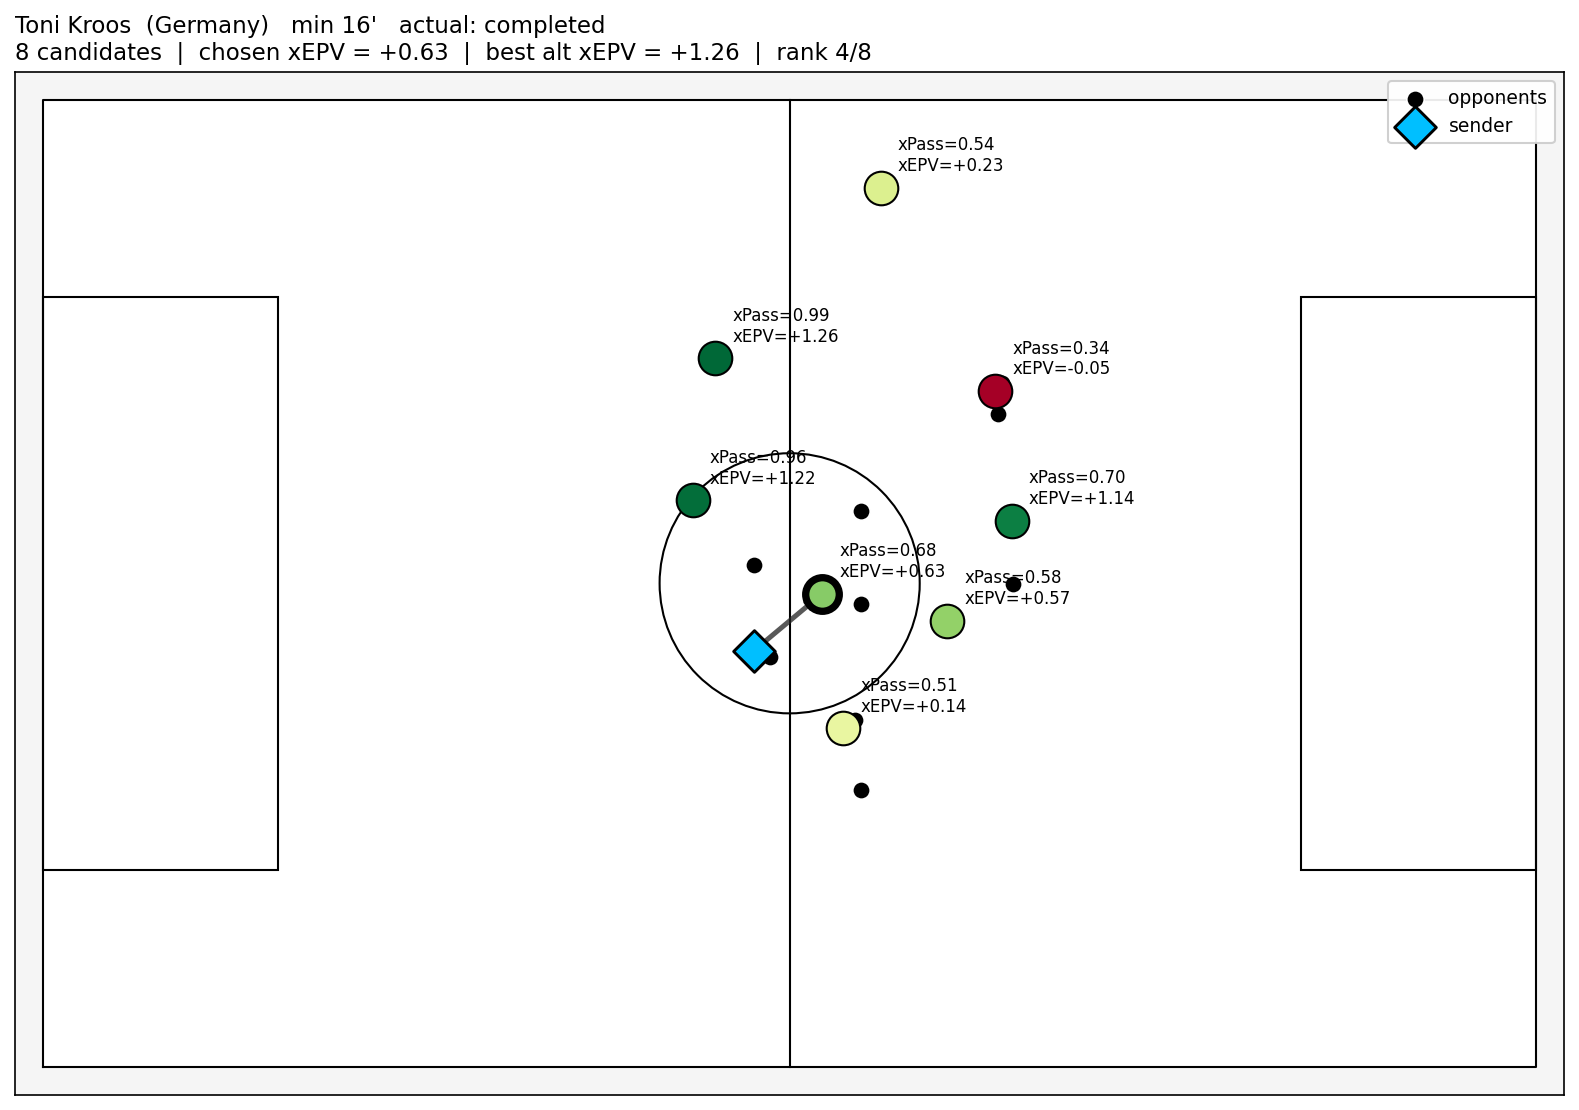
\includegraphics[width=\textwidth]{images/xepv_example.png}
        \caption{Same candidates coloured by xEPV.}
    \end{subfigure}
    \caption{The Kroos frame (Germany vs.\ Scotland, min~16): xPass vs.\ xEPV ranking reversal.  On the left the eight in-frame candidates are coloured by completion probability (red~=~low, blue~=~high); on the right the same candidates are coloured by xEPV (red~=~negative net value, green~=~positive).  The ranking changes because xEPV multiplies probability by destination value and subtracts the mirrored failure cost.}\label{fig:kroos-frame}
\end{figure}

\subsection{The 4-Axis Radar}\label{sec:dq-radar}

The DQ card mirrors the H1 family pattern: a magnitude headline (DQ index) next to a within-role percentile radar decomposing it behaviourally along four axes (all oriented so outside is better):
\begin{itemize}
    \item Picks the best: rate of in-frame value-optimal picks.
    \item Avoids the worst: rate of in-frame value-bottom picks, mirrored ($100 - \text{percentile}$).
    \item Elite reads\,/\,90: volume of top-decile decisions per 90.
    \item Avoids poor\,/\,90: volume of bottom-decile decisions per 90, mirrored.
\end{itemize}
These four split the single Score into the two things a scout actually wants separated: how good the picks are (accuracy and avoid-worst rates) and how often they happen (elite\,/\,90 and avoid-poor\,/\,90 volumes).
A core-stats table under the radar exposes the raw scout-facing values (Score, Value Impact, the four radar sources in raw units, average miss cost, and the number of decisions with minutes), so low-sample profiles can be discounted. (The ``average miss cost'' is the mean xEPV left on the table \emph{on the events that were sub-optimal}, representing the severity of a mistake, separate from its frequency.)

\begin{figure}[H]
    \centering
    
\includegraphics[width=0.8\textwidth]{images/dq_radar_example.png}
    \caption{Toni Kroos DQ radar.  Kroos sits at the 88th~percentile among MIDs on 379 decision events over 485~minutes.  The radar reads as the metronome profile: high Elite reads\,/\,90 (volume of top-decile picks), strong Avoids-the-worst (rarely the value-bottom alternative), solid Picks-the-best, more modest Avoids-poor\,/\,90 because the per-90 rate of bottom-decile decisions also carries his involvement volume.}\label{fig:dq-radar}
\end{figure}

\subsection{Validation}\label{sec:h2-validation}

\begin{enumerate}
    \item \textbf{Statistical robustness.} The entire pipeline is refit while moving, one at a time, the turnover scale ($s \in \{0.5, 1.0, 1.5\}$), the minutes floor ($90$, $135$, $180$~min), and the minimum-alternatives threshold ($\geq 1$, $\geq 2$, $\geq 3$). In each sweep the Spearman correlation of the player ordering against the shipped index exceeds $\rho \geq 0.95$: these knobs set the \emph{level} of the scores, not who ranks above whom.
    \item \textbf{Spatial sanity check.} The mean chosen xEPV by sender pitch zone is monotonically increasing with the sender's x-position: passes from advanced positions yield more net expected value on average, as the reward term grows and the mirrored failure cost shrinks. A reward-vs.-penalty decomposition by xPass decile confirms the expected dynamic: in the lowest-xPass decile both the reward ($\text{xPass} \cdot \text{EPV}$) and the penalty ($(1 - \text{xPass}) \cdot \text{EPV}_{\text{mirror}}$) are large, meaning players go for valuable targets and risk a costly turnover, while in the highest-xPass deciles the penalty collapses to near zero and the reward is what remains.
    \item \textbf{Construct validity.} The within-role correlation matrix of the radar axes confirms they are not duplicates, and two design claims are checked directly against the data (accuracy and worst-choice are near-independent rather than two sides of one coin).
    \item \textbf{Face validity.} Covered in the findings below.
\end{enumerate}

\subsection{Key Findings}\label{sec:h2-findings}

\paragraph{Confirmations: recognised passers land where football expects.}
Pedri (Spain, CAM) sits at the 95th percentile of DQ. He is the clearest pure selector of the tournament: not the loudest passer, but the one who consistently picks the best option his frame offers.
Toni Kroos (Germany, MID, $n=379$) at DQ~88th on the largest sample of any midfielder, with 10.6 elite reads\,/\,90 and only 4~worst-choice events per~100.
Kevin De Bruyne (Belgium, CAM, $n=136$) at DQ~85th, highest Picks-the-best\,\% at 17.6\%.
Mateo Kova\v{c}i\'{c} (Croatia, MID) at DQ~82nd.
\.{I}lkay G\"{u}ndoğan (Germany, CAM) at 70th.
Phil Foden (England, WIDE) and Rodri (Spain, MID) upper-mid at 68th and 65th.

\paragraph{Surprises: names the volume view never surfaces.}
Lesser-known players with DQ index $\geq 90$ on a meaningful sample ($n \geq 40$):
R\u{a}zvan Marin (Romania, MID, $n=68$) at DQ~98th, Picks-the-best 27.9\%, both very high in role.
Nacho Fern\'{a}ndez (Spain, CB, $n=86$) is at the 98th percentile of DQ. The Spain back-line is one of the discoveries of the tournament on this metric.
A cluster of centre-backs at the very top of the CB pool: Marin Pongra\v{c}i\'{c} (Croatia), Jack Hendry (Scotland), Jakub Kiwior (Poland), Jan Bednarek (Poland).
Four full-backs at DQ~$\geq 93$ on small but real samples: Mario Mitaj (Albania), Andrei Ra\c{t}iu (Romania), Otar Kakabadze (Georgia, highest Picks-the-best of the surprises at 30\%), Anthony Ralston (Scotland).
Cody Gakpo (Netherlands, WIDE, $n=83$) at DQ~95th, Picks-the-best 30.1\%.
Piotr Zieli\'{n}ski (Poland, MID), Joey Veerman (Netherlands, MID), and Giorgi Kochorashvili (Georgia, MID) sit at DQ 94--97 on $n \geq 97$, representing the most solid surprises of the MID pool.

\paragraph{Big names that do not measure up.}
Joshua Kimmich (Germany, FB, $n=256$) at DQ~10th, the lowest of the famous watchlist by a margin: high worst-choice\,\% (7.4) and high poor-reads\,/\,90 (5.2) on a very large sample.
Nicol\`{o} Barella (Italy, MID, $n=193$) at DQ~12th, Picks-the-best only 7.3.
Granit Xhaka (Switzerland, MID, $n=296$) at DQ~40th.
Luka Modri\'{c} (Croatia, MID, $n=169$) at DQ~45th, the most counter-intuitive low.
Declan Rice, Jude Bellingham (England), and Bernardo Silva (Portugal) are all in the upper-middle range (50--55), falling below public expectation but not low.

\paragraph{Declared scope limit: tempo controllers.}
Kimmich, Modric, Xhaka and Barella all play deliberate tempo control, and xEPV is a per-pass quantity with no game state (no scoreline, no clock, no tactical instruction), so a deliberately safe, possession-securing pass reads as a weak selection.
The metric does not see tempo management; the gap is in the lens, not necessarily in the player.
We state this openly rather than tuning it away.

\clearpage
% ============================================================
\section{H3: Off-Ball Movement}\label{sec:h3}
% ============================================================

H1 and H2 both judge a player \emph{on the ball}, but a player touches the ball for only a few minutes a match; the rest is movement. H3 turns to that off-ball majority.

\textbf{Hypothesis~3.}
Most of a player's game happens \emph{without the ball}, and the value of that work is invisible to event data.
We measure the dangerous off-ball space a player occupies that his teammates fail to use: high-value runs that are made, seen by the freeze frame, and left unserved.

\subsection{The URS Index}\label{sec:urs}

While a teammate has the ball, every other visible teammate is a \emph{candidate target} the ball-carrier could have served.
For each candidate we ask two questions:
\begin{enumerate}
    \item How much would that pass have been worth? We score it with the shared xEPV (\cref{eq:xepv}).
    \item Was the run actually served? A candidate is received if the next ball-touch within 4~seconds belongs to him. The 4-second window is empirically calibrated: the P95 of the observed pass-to-receipt time on completed passes across the tournament is approximately 3~seconds. Setting the window one second above P95 captures $\sim$96\% of genuine receipts while avoiding absorption of the next independent phase of play.  The exact value is not critical: rebuilding the URS\,/\,90 ranking for window values $N \in \{2, 3, 4, 5, 7\}$~seconds shows Spearman $\rho \geq 0.95$ against the $N=4$ reference on the immediate neighbours.
\end{enumerate}

The headline is the Uncapitalised Run Score:
\begin{equation}\label{eq:urs}
    \text{URS\,/\,90} = \frac{\displaystyle\sum_{f \in F_p} \text{xEPV}(f) \cdot (1 - \text{received}(f))}{\text{minutes}_p} \times 90,
\end{equation}
where $F_p$ is the set of confident candidate frames for player~$p$.
The full per-player aggregation also decomposes each event into three additive terms:
\begin{align}
    \text{off\_ball\_value}_i &= \text{xEPV}_i, \notag\\
    \text{urs}_i &= \text{xEPV}_i \cdot (1 - \text{received}_i), \notag\\
    \text{captured}_i &= \text{xEPV}_i \cdot \text{received}_i, \notag
\end{align}
so that $\text{Potential}_{/90} = \frac{\sum_i \text{off\_ball\_value}_i}{\text{minutes}} \times 90$, the capitalisation rate $\text{Cap.} = \frac{\sum_i \text{captured}_i}{\sum_i \text{off\_ball\_value}_i}$, and $\text{Latency} = 1 - \text{Cap.}$
The headline rating is its within-macro-role percentile.

\paragraph{Why ``uncapitalised.''}
The whole point of H3 is to find value the event log misses.
Value that was served already shows up downstream (someone received it and did something with it).
The interesting, invisible quantity is the value that was offered and \emph{wasted}, which is the run nobody played.
Multiplying each offered xEPV by $(1 - \text{received})$ isolates exactly that.

\subsection{The Two-Axis Decomposition}\label{sec:urs-decomp}

URS factors cleanly into two halves, which become two of the radar axes:
\begin{equation}\label{eq:urs-split}
    \text{URS\,/\,90} = \underbrace{\text{Off-Ball Potential\,/\,90}}_{\text{how much value he exposes}} \times \underbrace{\text{Latency}}_{\text{the share left unserved}}.
\end{equation}

A player with high Potential and high Latency is a \textbf{shadow runner}: he keeps offering dangerous options his team does not use.
A player with high Potential and low Latency is a \textbf{trusted threat}: he offers as much, and his team uses it.
The third radar axis is \textbf{xEPV mean} (the quality of his average offered frame), which separates a player who exposes a few great runs from one who exposes many ordinary ones.
We are honest about one dependency: Off-Ball Potential correlates with the URS headline at about $\rho \approx 0.97$ by construction (since $\text{URS} = \text{Potential} \times \text{Latency}$ and Potential carries the wider spread). We keep Potential on the radar anyway, as the most \emph{readable} volume axis, rather than pretending it is an independent signal. This represents the same honesty H2 applies to its Value Impact companion.

\paragraph{Declared dependency: conditional on teammate execution.}
URS carries a structural interpretation constraint that we state plainly: it is conditional on teammate execution.
A candidate counts toward URS only when the run is not served. Whether a run is served depends partly on the ball-carrier (their vision and execution) and not on the off-ball player alone.
Crucially, the constraint does not spread evenly across the metric:
\begin{itemize}
    \item \textbf{Off-Ball Potential} is the player-only half: it depends on where he moves and the danger of the space he occupies, not on whether anyone serves him.
    \item \textbf{Latency} is the half where teammate execution enters.
\end{itemize}

The within-role correlation between the two axes is only $\rho \approx 0.08$ (i.e., how much space a player exposes is empirically almost independent of whether it gets used).
We also tested the environment effect directly: correlating each player's Latency with the leave-one-out mean H2 Decision-Quality of his own teammates gives $\rho \approx -0.13$ (significant, direction correct, indicating that better teammates capitalise more, but small, explaining only ${\sim}2\%$ of variance).
URS remains predominantly a player signal, with the environment a measurable but minor contributor.

\paragraph{URS as a complement to H2.}
H2 grades a player as the server, measuring how well he chooses among the options he has on the ball.
H3's Latency grades the same kind of event from the other side: how often a player's off-ball offers are \emph{not taken by his teammates}.
Read together they are informative precisely \emph{because} URS is conditional on the environment: a player with high Off-Ball Potential surrounded by low-H2 teammates is one whose off-ball value is being systematically under-used by his current side, representing an actionable scouting signal.

\subsection{The Receiver Resolver}\label{sec:resolver}

This is the methodological core of H3, and the reason off-ball rating is normally considered impossible from public data.

\paragraph{The problem.}
A 360~frame gives positions but no identity: only the player on the ball is named; everyone else carries just a team tag.

\paragraph{The three-step resolver.}
\begin{enumerate}
    \item Estimate each teammate's position at the instant of the pass by bracket interpolation. A 360~frame freezes the dots but does not name them; what is named, elsewhere in the event log, is every moment a player touches the ball. So for each teammate we find his nearest on-ball event before the pass and his nearest one \emph{after} it, and we read off where he must have been at the pass instant by interpolating linearly between those two known points (in both position and time). The intuition is simple: if a player was at point A two seconds before the pass and at point B one second after, his location at the pass is a weighted point on the segment A--B. This ``v2'' bracket method replaced a ``v1'' baseline that used only his last-known position before the pass (a backward-only guess that goes stale the moment he keeps running); bracketing is far more accurate because it pins the estimate between two real observations rather than extrapolating from one, effectively using the player's own trajectory on both sides of the instant as a short motion prior. Only events inside the staleness window (\cref{sec:sweeps}) are used, so a stale bracket is never trusted.
    \item Match estimates to dots with the Hungarian algorithm~\cite{hungarian}. We now have a set of estimated teammate positions and a set of anonymous same-team dots in the frame, and we must decide which estimate is which dot. This is a one-to-one assignment problem, and the Hungarian algorithm solves it optimally: it finds the pairing of estimates to dots that minimises the total distance over all pairs at once. A simpler greedy rule (give each estimate its nearest free dot, one at a time) can paint itself into a corner, assigning an early dot cheaply and forcing a later estimate onto a far-away wrong dot; minimising the global total avoids that trap.
    \item \textbf{Keep only confident assignments.} An assignment is kept only if its estimate lands within 8\,m of the matched dot; everything looser is discarded and never scored. This is the knob that trades coverage for reliability (\cref{sec:sweeps}): tightening it raises accuracy but drops more candidates.
\end{enumerate}

\paragraph{Validation.}
There is no ground truth for off-ball runs, but there is ground truth for completed passes: the recipient is named.
So we validate where truth exists and carry the result over: we hide the recipient, let the resolver predict which dot is the receiver, and check it against the real name.
On the open-play universe the metric runs on, the bracket resolver reaches 93.2\% accuracy on the confident assignments it keeps, far above the ${\sim}74\%$ of the naive last-known-position baseline.

This number is not just descriptive; it is a decision gate. The accuracy sets the granularity at which H3 is allowed to report: if accuracy-on-confident clears an 85\% bar, the resolver is trusted to name individual dots and H3 reports a per-player URS ranking (``Tier~1''); below that bar it would fall back to coarser zone- and role-level aggregates (``Tier~2''), where a wrong identity does less damage. At 93.2\% the bar is cleared comfortably, which is what licenses the per-player leaderboards in the rest of this section.

\subsubsection{Parameter Sweeps}\label{sec:sweeps}

Two thresholds govern the resolver, and both were calibrated (a 10-match sweep is in the notebook):
\begin{itemize}
    \item \textbf{Staleness window: 5~seconds.} A teammate's position is only estimated from an event within this many seconds of the pass. Sweeping the window from 20\,s down to 5\,s, accuracy on confident dots rises from 88\% to 96\% while the volume of confident candidates stays essentially flat (${\sim}1.0\times$). So tightening the window buys fresher, more accurate estimates at no cost in coverage, representing an unusually clean trade. The final URS\,/\,90 player ranking is stable across the whole window range (Spearman $0.96$ versus the 20\,s setting).
    \item \textbf{Confidence threshold: 8\,m.} At 8\,m the mean localisation error of confident dots is about 4\,m and accuracy ${\sim}96\%$. Tightening to 6\,m does not raise accuracy but throws away ${\sim}17\%$ of candidates, showing that 8\,m is the point that keeps the most data without sacrificing accuracy.
\end{itemize}

A practical note on reproducibility: because StatsBomb regenerated every event UUID, H3 cannot merge onto H2's frozen alternatives table (it would return zero rows). Instead it recomputes xPass on the fly from the live freeze frames using H2's saved model (the same model with the same 12 features), so the value attached to each candidate is exactly what H2 would attach (median difference $0.000$ on shared events).

\subsection{Validation}\label{sec:h3-validation}

\paragraph{Split-half reliability.}
Splitting the 51~matches by date into the first 25 and last 26, the URS\,/\,90 ranking reproduces at Spearman $\rho = 0.72$ ($n=117$ players who clear the floor in both halves), as visualised in the scatter plot of \cref{fig:urs-split-half}.
A player's URS over the opening matches predicts his URS over the closing ones, which is the key reliability check for a metric built on a thin behavioural signal. It establishes that the metric captures a stable individual skill rather than temporary run-to-run noise.

\begin{figure}[H]
    \centering
    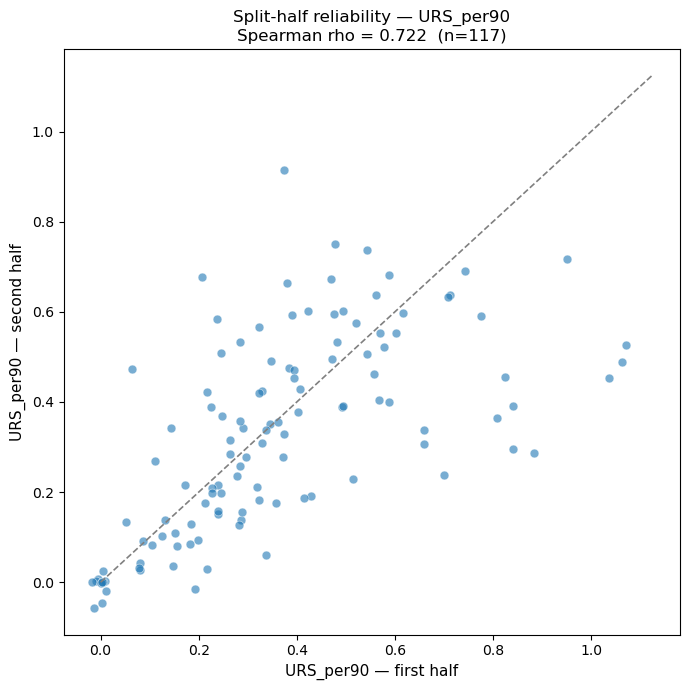
\includegraphics[width=0.85\textwidth]{images/urs_split_half.png}
    \caption{Split-half reliability of the Uncapitalised Run Score (URS\,/\,90) across Euro 2024. The 51 matches were split chronologically (first 25 vs.\ last 26), and player rankings were compared for the $n=117$ players who played at least 90 minutes in both halves. The high Spearman correlation ($\rho \approx 0.72$) confirms the index captures a stable on-pitch signal rather than random variation.}\label{fig:urs-split-half}
\end{figure}

\paragraph{Axis independence.}
The within-role Spearman correlation of the three radar axes (\cref{tab:h3-corr}) confirms that Off-Ball Potential and Latency are almost unrelated ($\rho \approx 0.08$): how much space a player exposes is essentially independent of whether it gets used, which is the empirical heart of the shadow-runner idea.

\begin{table}[H]
\centering
\caption{Within-role Spearman correlation of H3 radar axes.}\label{tab:h3-corr}
\small
\begin{tabular}{@{}lrrr@{}}
\toprule
& \textbf{Potential\,/\,90} & \textbf{xEPV mean} & \textbf{Latency} \\
\midrule
\textbf{Potential\,/\,90} & 1.00 & 0.56 & 0.08 \\ \midrule
\textbf{xEPV mean} & 0.56 & 1.00 & 0.15 \\ \midrule
\textbf{Latency} & 0.08 & 0.15 & 1.00 \\
\bottomrule
\end{tabular}
\end{table}

\subsection{Key Findings}\label{sec:h3-findings}

\paragraph{The shadow runners.}
Pedri (Spain, CAM, $n=185'$) tops the whole pool at URS\,/\,90 $= 2.78$, roughly twice the next name.
He exposes more off-ball value than anyone (Potential\,/\,90 $= 3.30$) and is served on only 16\% of it: the extreme shadow runner of the tournament.
Behind him Jorginho ($1.41$), Hjulmand ($1.08$) and Modric ($0.92$) are the recognised tempo-setters of the tournament, and Kimmich ($0.85$), Wirtz ($0.84$) and Kroos ($0.82$) follow.

\Cref{fig:uncap-pedri} is the on-pitch proof of what URS counts. Each panel is one of Pedri's four highest-URS moments: he (green) has found dangerous space inside or just outside the opponent block (red hull), the ball-carrier (cyan) has the ball and a clear passing lane, yet plays elsewhere, and the run goes unserved. The xEPV of each missed pass is the value left on the table, and summing it is the URS.

\begin{figure}[H]
    \centering
    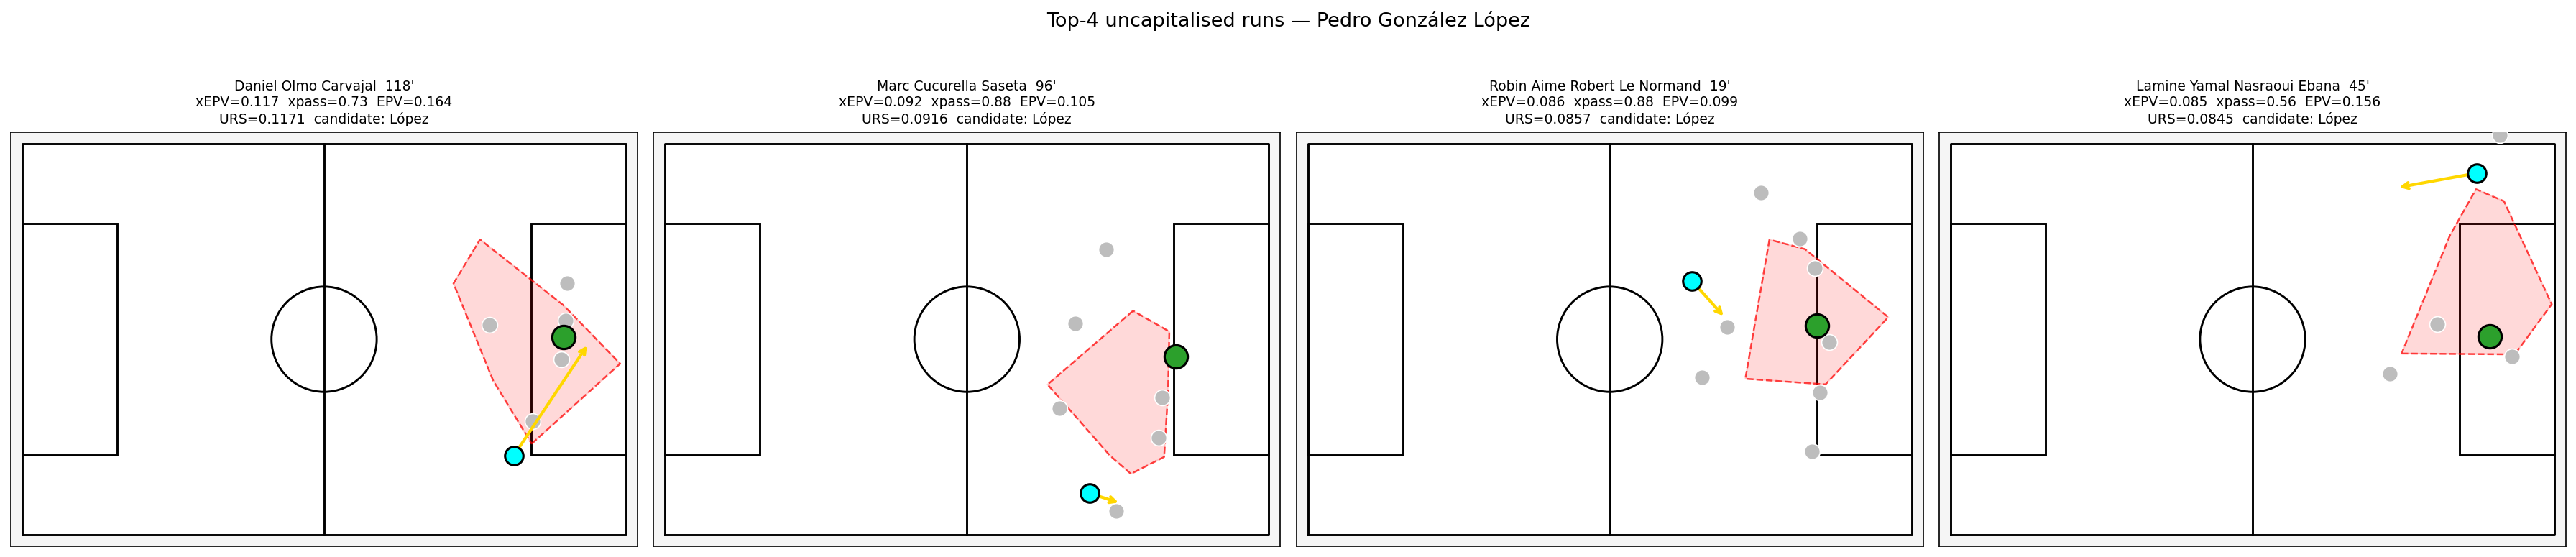
\includegraphics[width=\textwidth]{images/uncapitalised_runs_pedri.png}
    \caption{Visual proof of the Uncapitalised Run Score: Pedri's four highest-URS off-ball moments at Euro 2024. In each frame Pedri (green) occupies dangerous space relative to the opponent block (red convex hull); the ball-carrier (cyan, with the yellow arrow showing the pass he actually played) has him available but serves a different option, so the run is not capitalised. Each panel's xEPV is the net value the unserved pass would have carried; the URS is the sum of these missed values per 90 minutes.}\label{fig:uncap-pedri}
\end{figure}

\paragraph{Why the absolute board is midfield-heavy.}
The absolute leaderboard is dominated by midfielders.  This is not a quirk but a structural consequence of three compounding effects:
\begin{enumerate}
    \item Midfielders appear as candidate teammates in more freeze frames, since they are simply seen more often by the resolver.
    \item They operate in higher-EPV zones than centre-backs, so their hypothetical xEPV is structurally larger.
    \item They are the easiest targets for the Hungarian assignment: most events happen near them, so position estimates are fresher and the confident flag is set more often.
\end{enumerate}
All three effects compound and concentrate URS\,/\,90 in the MID role.  The reading position by position is therefore the honest one, comparing a forward against a forward, a centre-back against a centre-back.

\paragraph{Within-role tops: where football already expects them.}
The role pools surface the right archetypes (none need the index to be recognised, which is itself a face-validity check):
\begin{itemize}
    \item CB: Tah, R\"{u}diger, Calafiori, R\'{u}ben Dias, Bastoni: the ball-playing centre-backs who step out and offer a forward option.
    \item FB: Kimmich, Dalot, Mittelst\"{a}dt, Di Lorenzo, Trippier: the attacking full-backs.
    \item MID: Jorginho, Hjulmand, Modri\'{c}, Kroos, Andrich: the creative engine room.
    \item CAM: Pedri, G\"{u}ndoğan, Eriksen: the between-the-lines tens.
    \item WIDE: Wirtz, Concei\c{c}\~{a}o, Foden, Su\v{c}i\'{c}, Musiala: the inside-drifting forwards.
    \item FW: Gregoritsch, Havertz, G\"{u}ler, Thuram, Oyarzabal.
\end{itemize}

\begin{figure}[H]
    \centering
    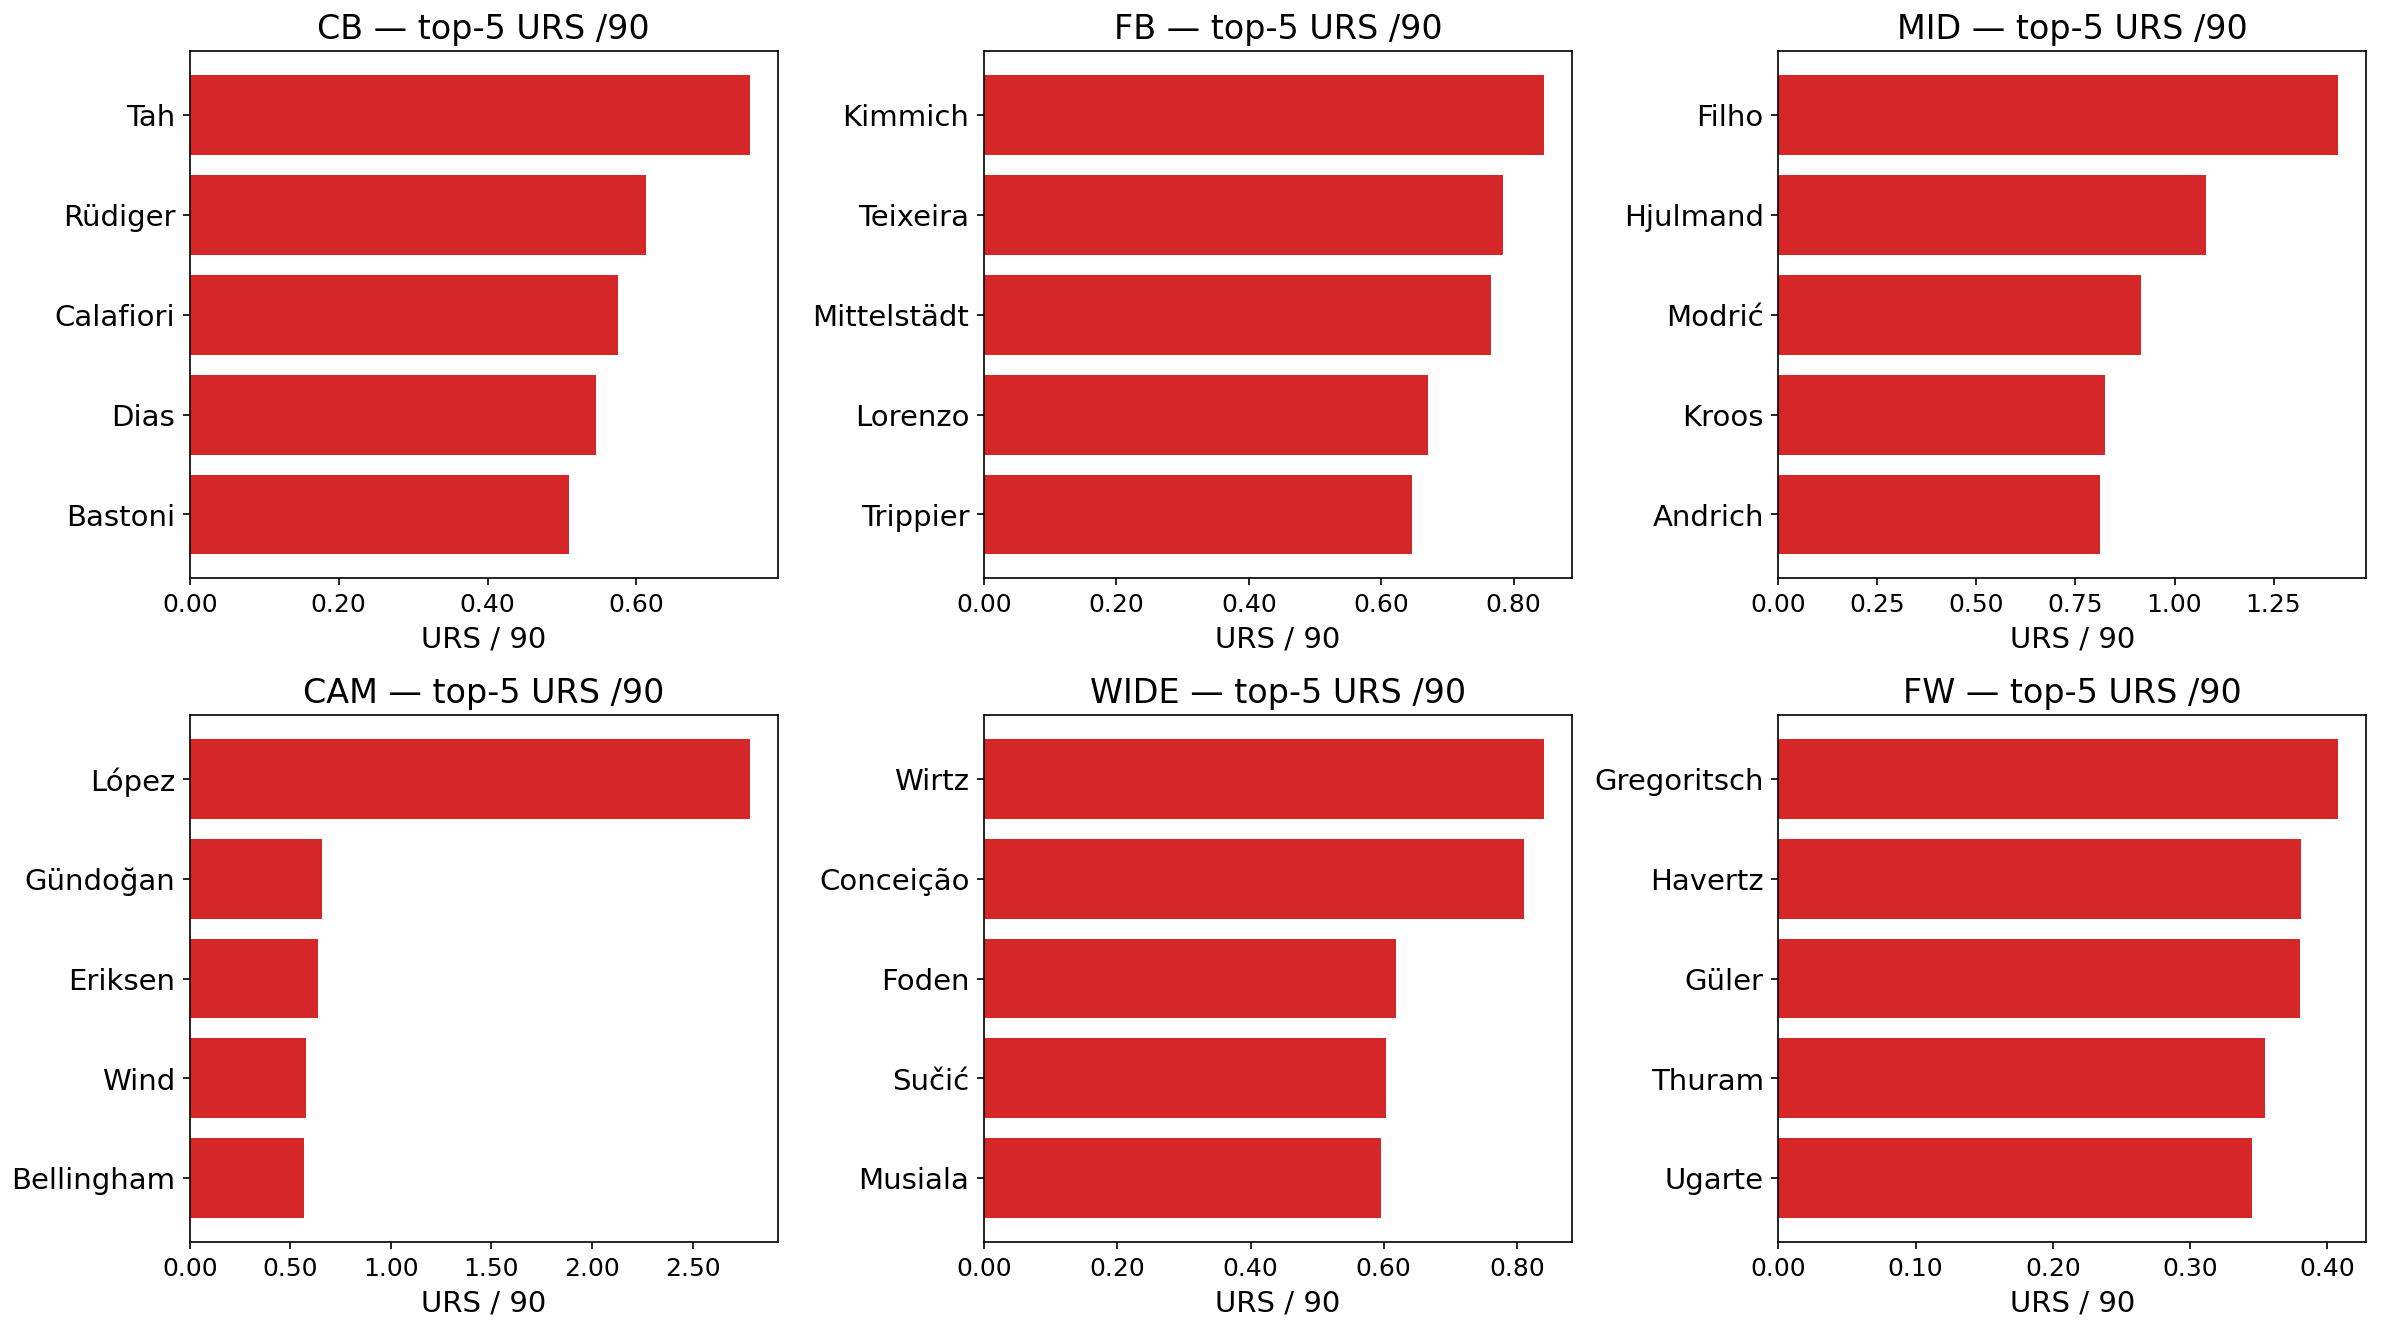
\includegraphics[width=\textwidth]{images/within_role_top5.png}
    \caption{Within-role top-5 by URS\,/\,90.  Each bar shows the URS\,/\,90 value for the top-5 players inside each macro-role, confirming that the right archetypes surface in every role pool: ball-playing CBs, attacking FBs, creative midfielders, between-the-lines tens, inside-drifting wingers, and dropping forwards.}\label{fig:within-role-top5}
\end{figure}

\paragraph{Trusted threat vs.\ shadow runner.}
The cleanest illustration is Pedri against Kroos.
Both are near the top on Off-Ball Potential, so on the volume axis they look alike.
The difference is Latency: Pedri is served on 16\% of the value he offers, Kroos on 50\%.
Same exposure, opposite outcome: one a threat his team keeps missing, the other a threat his team uses.

\begin{figure}[H]
    \centering
    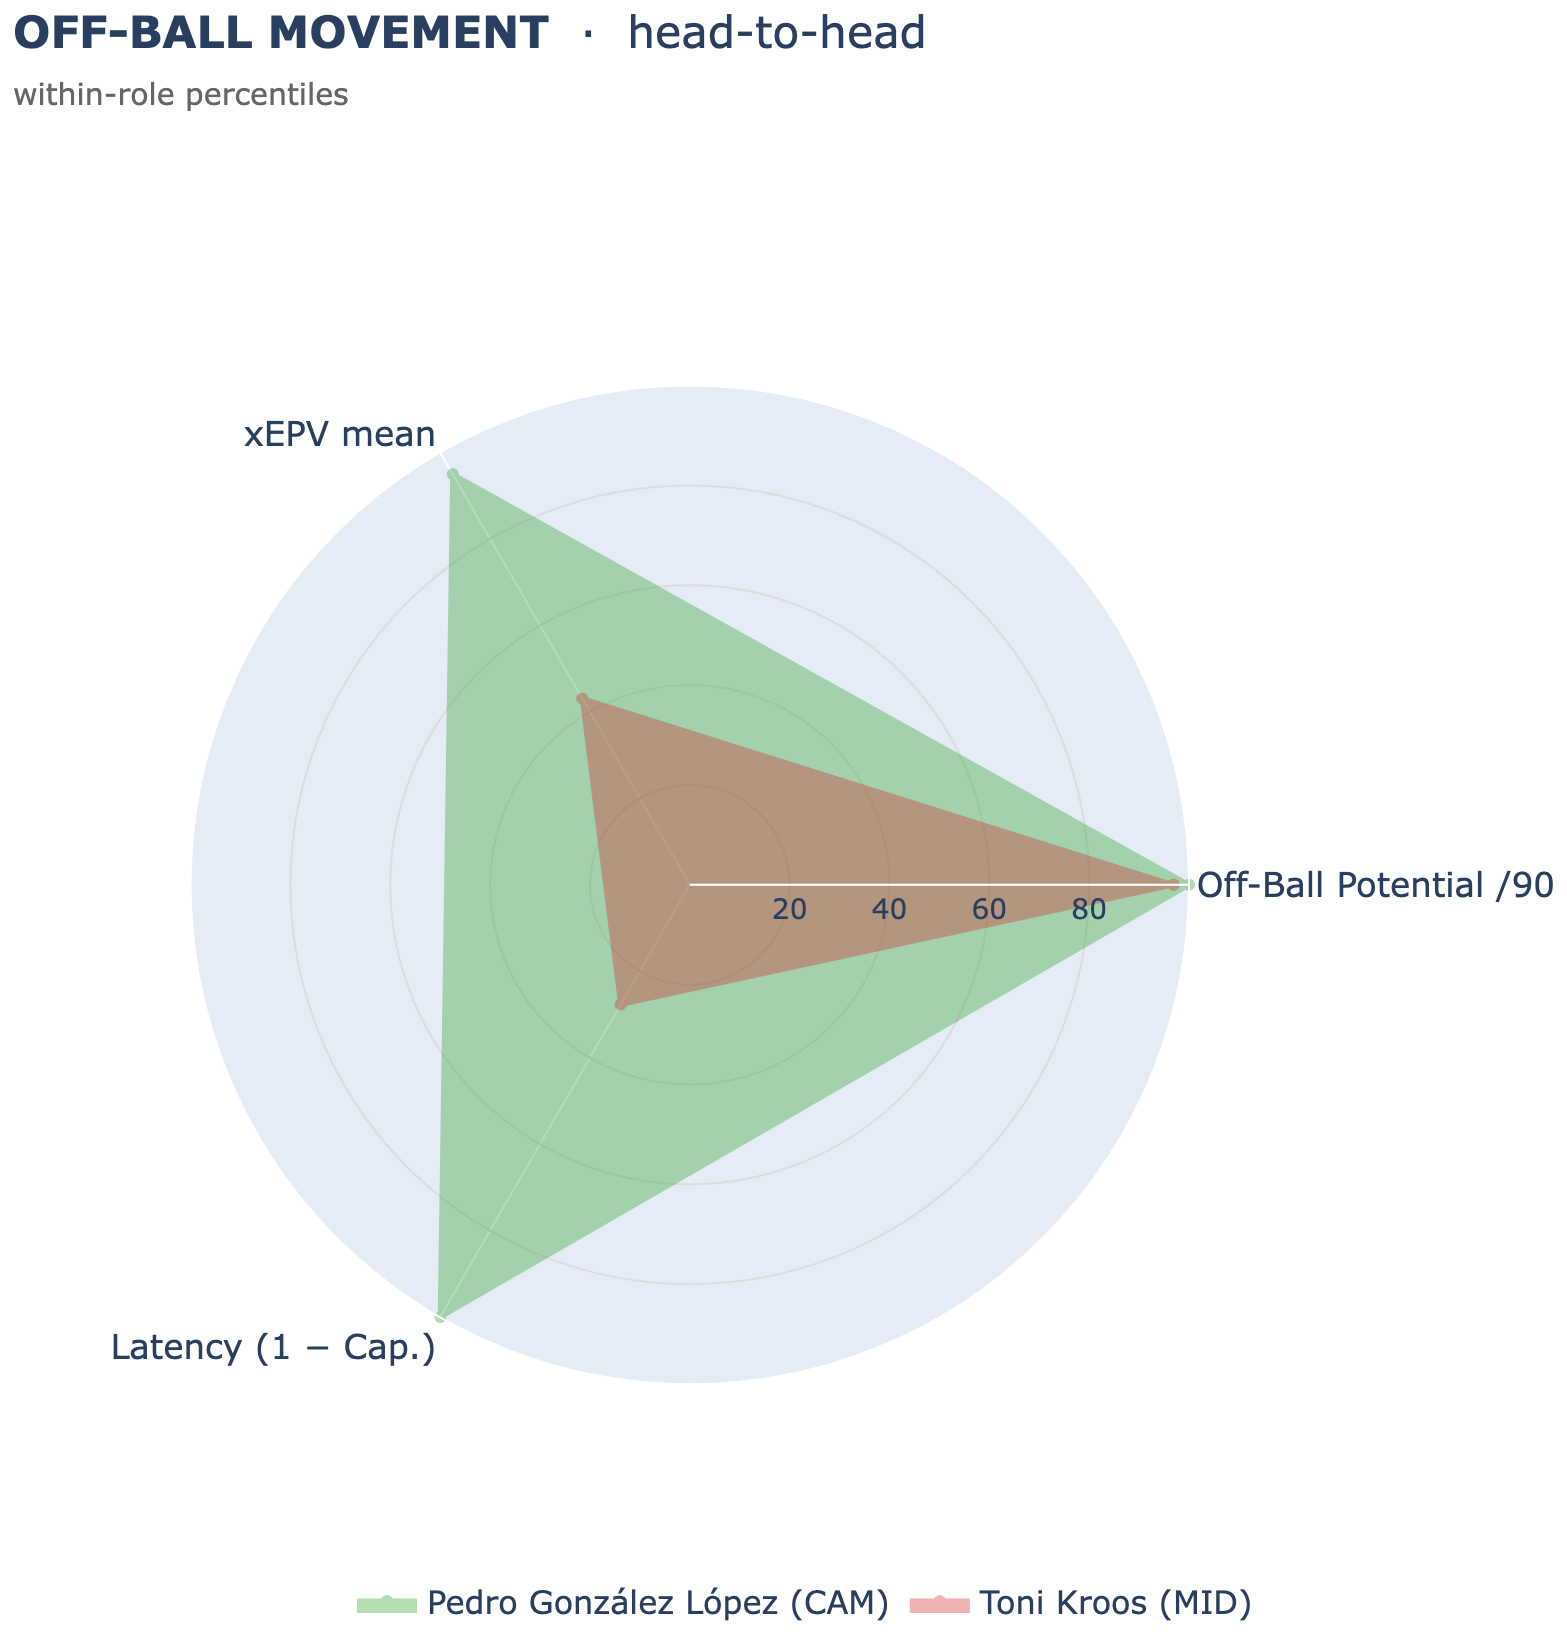
\includegraphics[width=\textwidth,height=0.82\textheight,keepaspectratio]{images/h2h_pedri_kroos.png}
    \caption{Pedri vs.\ Kroos head-to-head radar.  Both polygons overlap on Off-Ball Potential (volume axis) but pull apart on Latency: Pedri is served on only 16\% of his offered value (high latency, polygon stretched to the edge), Kroos on 50\% (lower latency, polygon pulled inward).  Same exposure, opposite team outcome.}\label{fig:h2h}
\end{figure}

\begin{figure}[H]
    \centering
    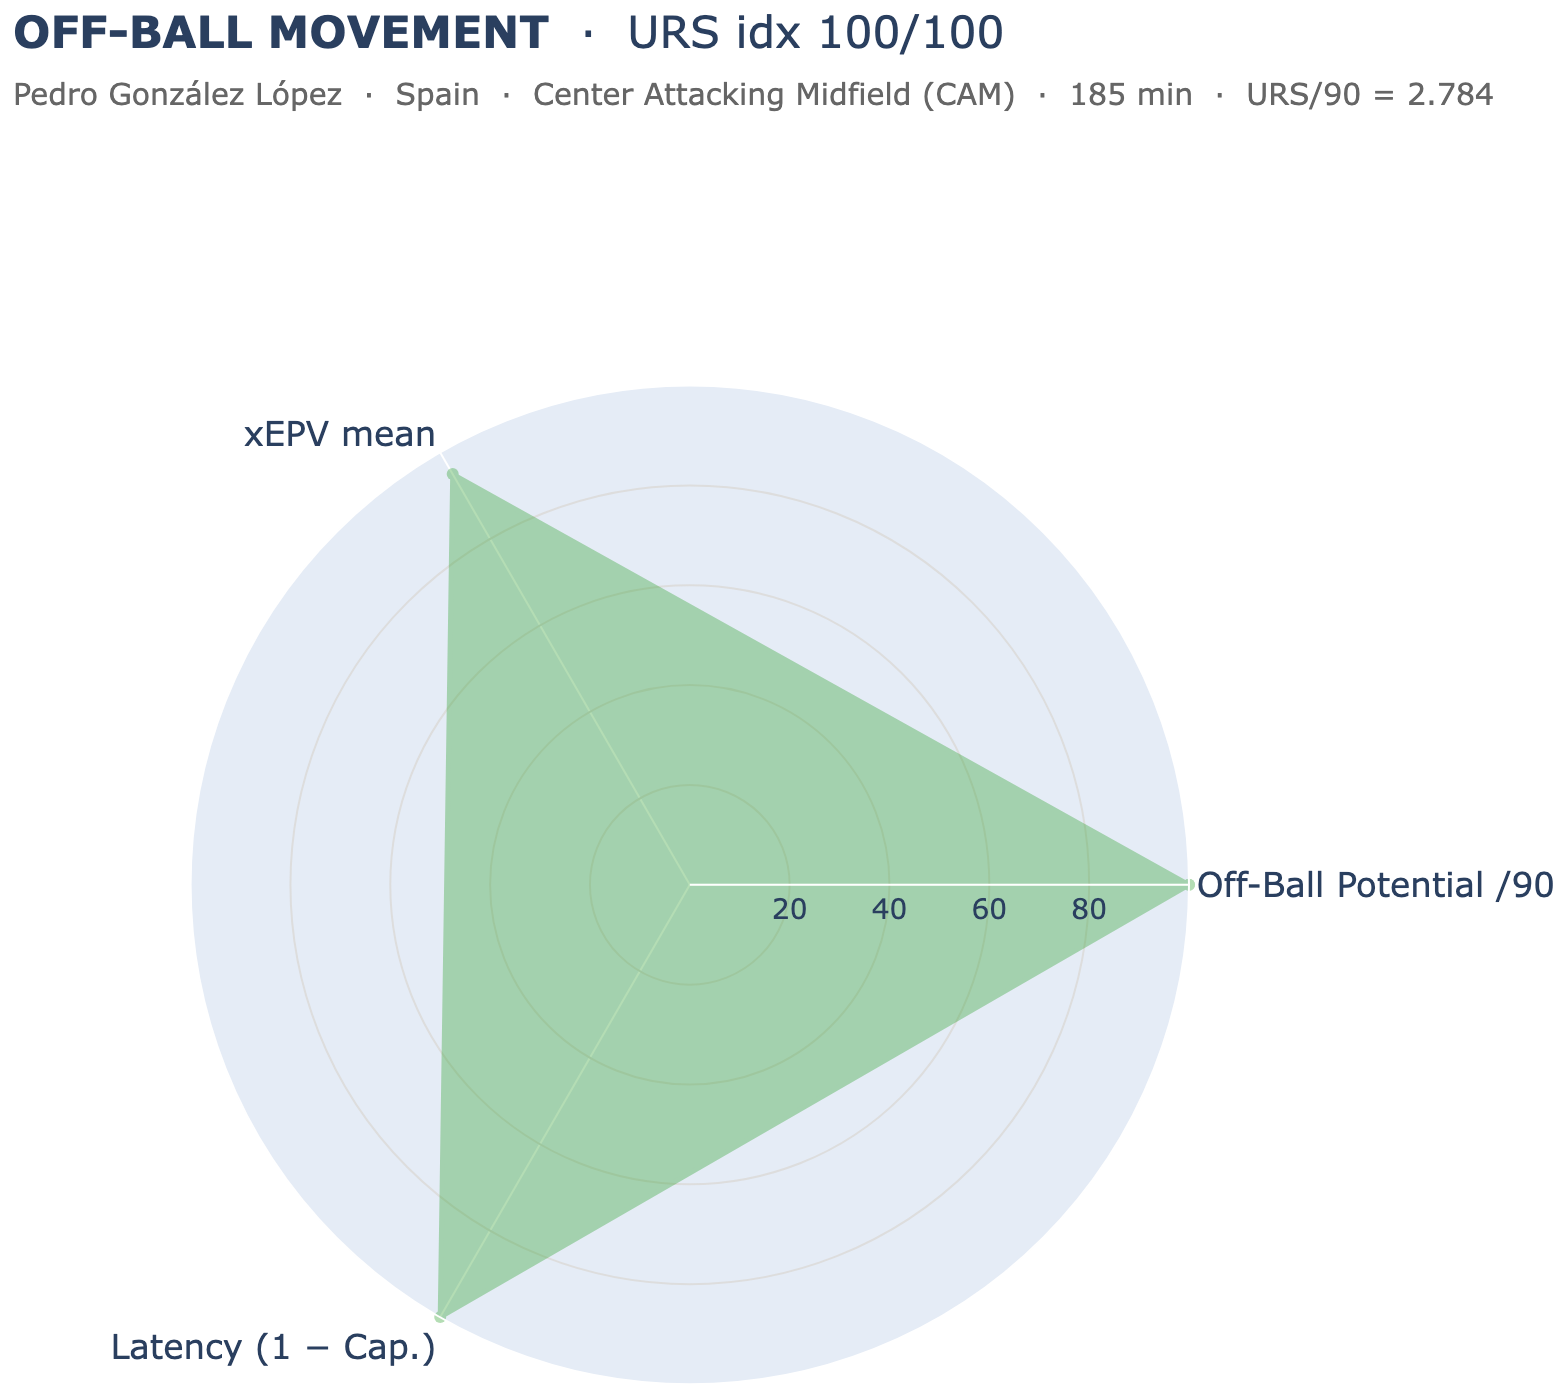
\includegraphics[width=\textwidth,height=0.78\textheight,keepaspectratio]{images/offball_radar_pedri.png}
    \caption{Pedri's off-ball radar.  He sits at the 100th~percentile of CAMs: maximum Off-Ball Potential, near-maximum xEPV mean, and the highest Latency of his role.  The shape is the extreme shadow-runner fingerprint, representing a player who exposes more dangerous space than anyone and is served on barely 16\% of it.}\label{fig:offball-pedri}
\end{figure}

\begin{figure}[H]
    \centering
    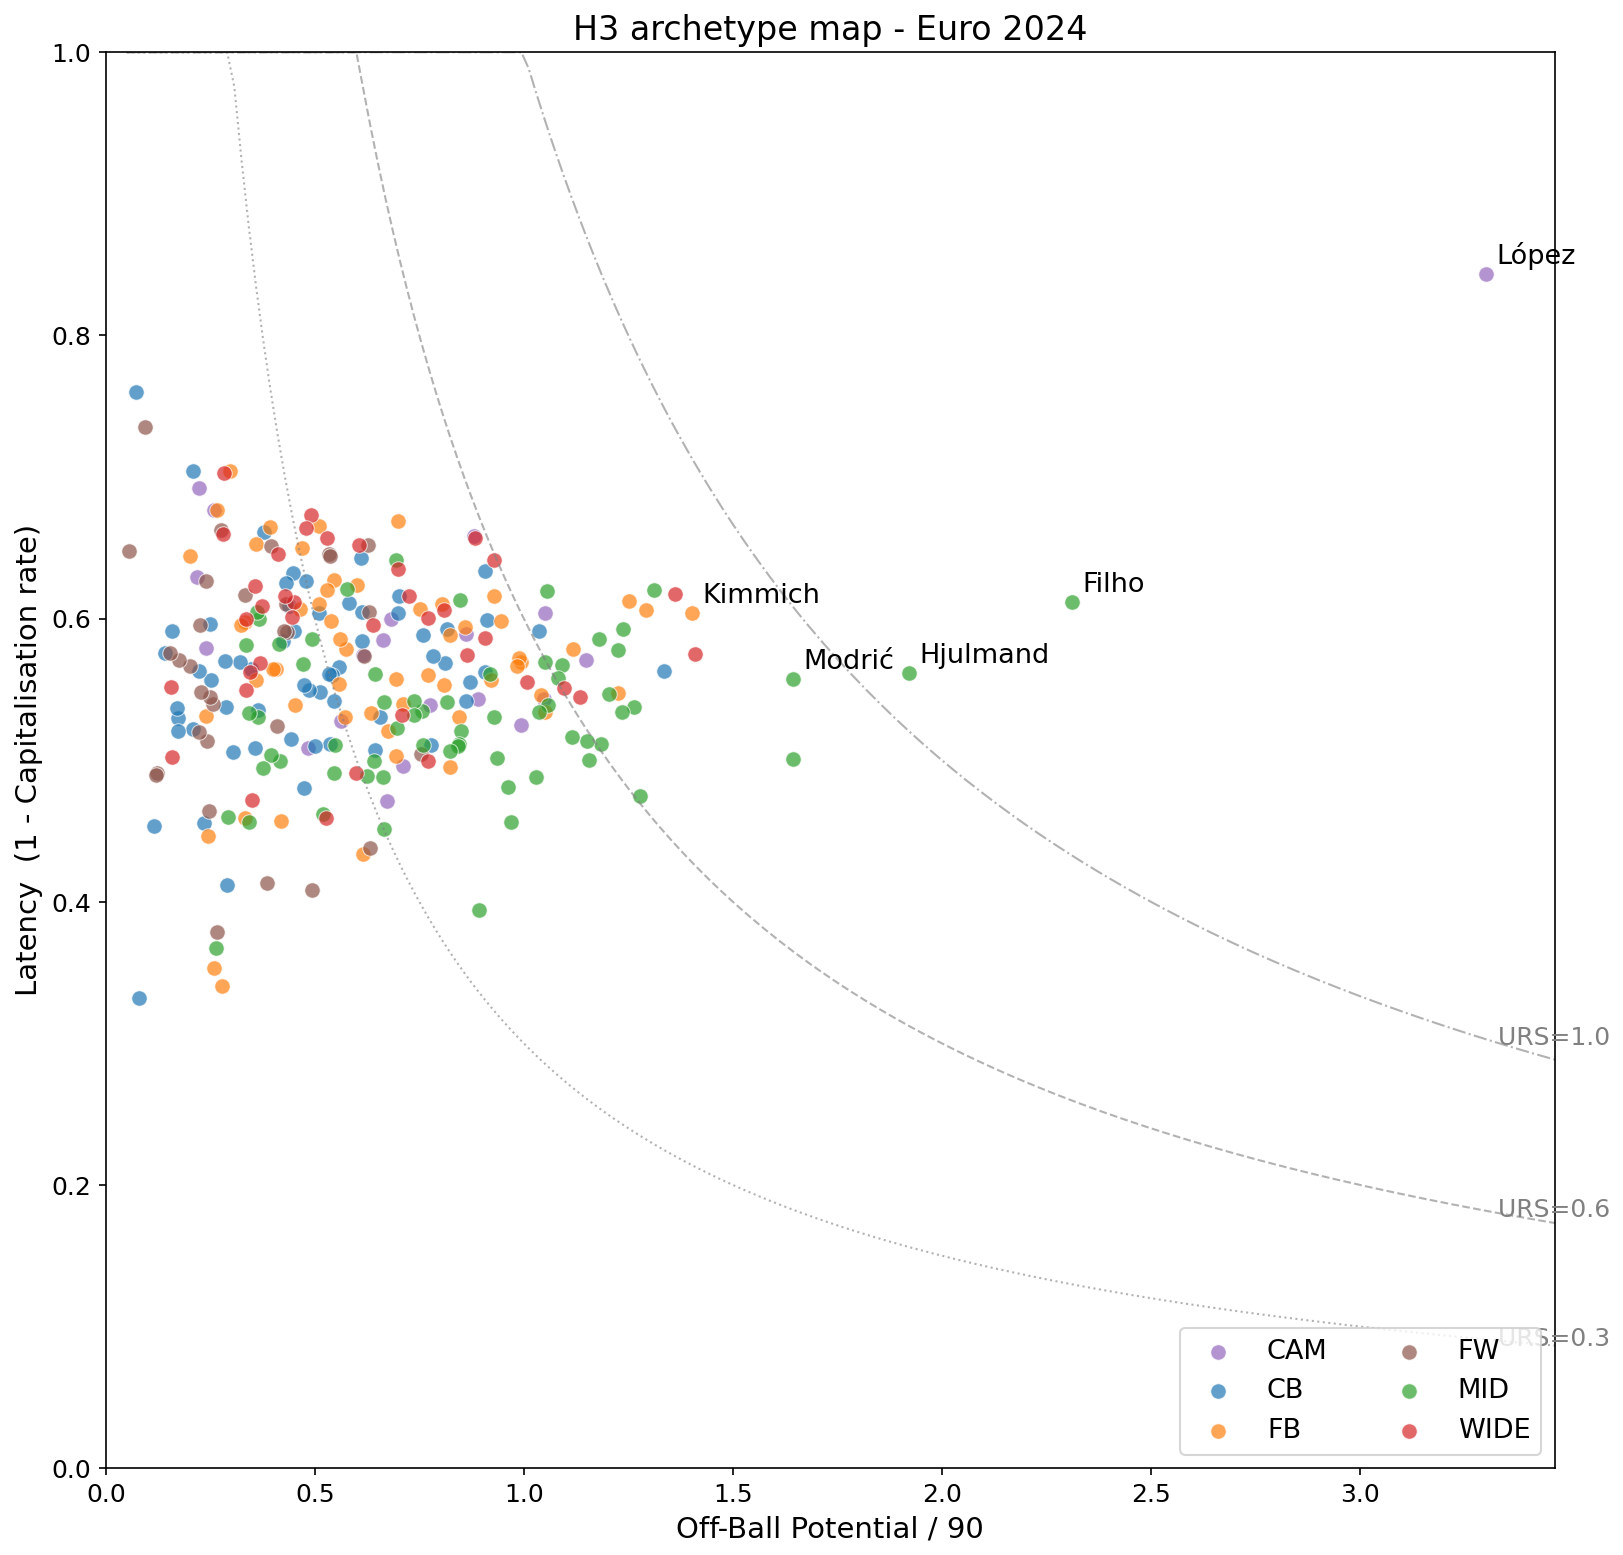
\includegraphics[width=\textwidth,height=0.78\textheight,keepaspectratio]{images/archetype_map.png}
    \caption{Archetype map: Off-Ball Potential vs.\ Latency. Each point is a player, colour encodes macro-role. The product $\text{Potential} \times \text{Latency}$ gives URS\,/\,90 directly; iso-URS curves are drawn as reference hyperbolas. Pedri sits alone in the top-right corner (high Potential, high Latency, representing the shadow runner); Jorginho, Hjulmand and Modric form the next cluster at middling Latency near 0.55; most players live below Potential $1.0$ with Latency in a narrow band, so the axis that moves a player out of the pack is exposure, not capitalisation.}\label{fig:archetype-map}
\end{figure}

\clearpage
% ============================================================
\section{H4: Player Similarity}\label{sec:h4}
% ============================================================

H1, H2 and H3 each rate a player; together they leave him described by a rich, team-bias-corrected feature vector. H4 stops rating and starts \emph{comparing}: it uses that vector to ask which players resemble each other.

\textbf{Hypothesis~4.}
With the three contextual metrics now in place, a player is already represented as a rich, team-bias-corrected feature vector.
H4 compares players by their intrinsic ``spatial DNA'' and behavioural playing style, rather than by nominal positional label, and powers a within-role similarity model that surfaces cost-effective alternatives with comparable tactical intelligence to premium assets.
This is the direct realisation of the value-arbitrage business case stated in \cref{sec:business}.

\subsection{From Clustering to Similarity}\label{sec:h4-from-clustering}

The project proposal framed H4 as a clustering problem: group the 272~players into emergent archetypes (e.g.\ via K-Means) on the contextual feature space.
We implemented and tested this, and on a single-tournament sample it proved degenerate.
Clustering \emph{across} all roles simply rediscovers the positional labels (defenders cluster with defenders), recovering nothing the macro-role already encodes; clustering within a role runs into pools too small (20--65 players) to yield stable groups, with cluster membership flipping under small perturbations.
We therefore pursue the same objective \emph{directly}, through a per-player nearest-neighbour similarity model: rather than imposing fragile archetype boundaries, we answer the scouting question one player at a time, namely \emph{given this player, who are his closest stylistic matches inside his own role?}

\subsection{The Player DNA}\label{sec:h4-features}

Each of the 272~players is described by an 11-dimensional DNA vector, assembled from the radar axes of the three earlier studies: the four H1 spatial indices (Progression, Dangerousness, Reception, Gravity), the four H2 decision-quality axes (Picks-best, Avoids-worst, Elite reads\,/\,90, Avoids-poor\,/\,90), and the three H3 off-ball axes (Off-Ball Potential, xEPV mean, Latency).
The two headline aggregates, H2's DQ~index and H3's URS\,/\,90, are deliberately excluded: each is a function (a rank, or the product $\text{Potential} \times \text{Latency}$) of axes already in the vector, so including them would double-count the same signal.
Because every axis is already a within-role percentile, the vector is naturally comparable, and within a role each dimension carries an equal share of the distance.
One adjustment is needed first: the H2 and H3 axes ship as uniform percentiles, but the H1 indices are composite scores with a tighter, non-uniform spread, so left unadjusted they would weigh less in a Euclidean distance (Gravity worst of all, at $3.7\%$ of the distance instead of $1/11 \approx 9.1\%$).
We therefore re-rank every axis to a within-role percentile before measuring distance, putting all eleven on one uniform $[0,100]$ scale; without this, the single closest match flips for $26\%$ of players.

\subsection{Similarity Model}\label{sec:h4-similarity}

Players are compared within macro-role only: the axes are within-role percentiles, so a percentile in one role is not commensurable with the same percentile in another, and cross-role distances would be ill-defined.
The dissimilarity of two players is the Euclidean distance between their DNA vectors, $d(A,B) = \sqrt{\sum_{i=1}^{11}(a_i - b_i)^2}$, mapped to a $0$--$100$ \textbf{similarity score}:
\begin{equation}\label{eq:h4-similarity}
    \text{similarity}(A,B) = \left(1 - \frac{d(A,B)}{D}\right) \times 100, \qquad D = \sqrt{11} \times 100 \approx 331.7,
\end{equation}
where $D$ is the largest distance two percentile vectors could ever have (every axis maximally apart).
Fixing $D$ to this theoretical maximum, rather than to the closest/furthest \emph{observed} pair (a min--max rescaling), makes the score stable and absolute: it depends only on the two players compared, so adding or removing others never shifts it, and a given score always means the same thing.
The cost is only cosmetic: real pairs occupy roughly the $23$--$88\%$ band rather than the full range, since two real footballers are never identical and never total opposites.
Combined with the Transfermarkt market values from \cref{sec:transfermarkt}, this operationalises the value-arbitrage use case: for a premium target, the model surfaces his cheaper stylistic look-alikes. The dashboard shows \emph{both} market values next to each match, the pre-Euro and the post-Euro price, alongside the player's age, so a scout reads the full valuation picture at a glance. The two values answer different questions and are both useful: the pre-Euro price is what a club could have paid before the tournament revealed the player's quality (the true arbitrage figure), while the post-Euro price shows where the market moved afterwards, which both updates the asking price today and lets the scout see whether a cheap look-alike has already started to appreciate.

\subsection{Validation}\label{sec:h4-validation}

Four checks confirm the similarity reads style rather than an artefact of the role pool.
\begin{enumerate}
    \item \textbf{Axes are not double-counting.} The within-role $|$Spearman$|$ matrix of the eleven axes peaks at $0.66$ (Avoids-poor\,/\,90 vs.\ Off-Ball Potential) with most pairs far lower; the few that stand out are football-sensible (a player who avoids poor decisions and reads space well tends to have high off-ball potential). None is high enough to be redundant, so all eleven are kept and the overlap is flagged, the same approach H2 and H3 apply to their own radars.
    \item \textbf{Style, not team.} Only $10.3\%$ of nearest matches are teammates; were the metric reading ``same side'' this share would be high.
    \item \textbf{No single axis carries it.} Dropping each axis in turn and re-checking the top-5 matches, the matches survive $83.5\%$ of the time. (The leaner 6-axis alternative, one number per headline concept, drops to $72.8\%$ and pairs players who reach the same overall level in very different ways, which is why the full 11-axis DNA is kept.)
    \item \textbf{It separates players.} Best-match scores spread properly (median $79$, range $65$--$88$): $14$~players have a strong stylistic twin ($>85$) while $47$ are more one-of-a-kind ($<75$), exactly the shape a discriminating metric should produce.
\end{enumerate}

\begin{figure}[H]
    \centering
    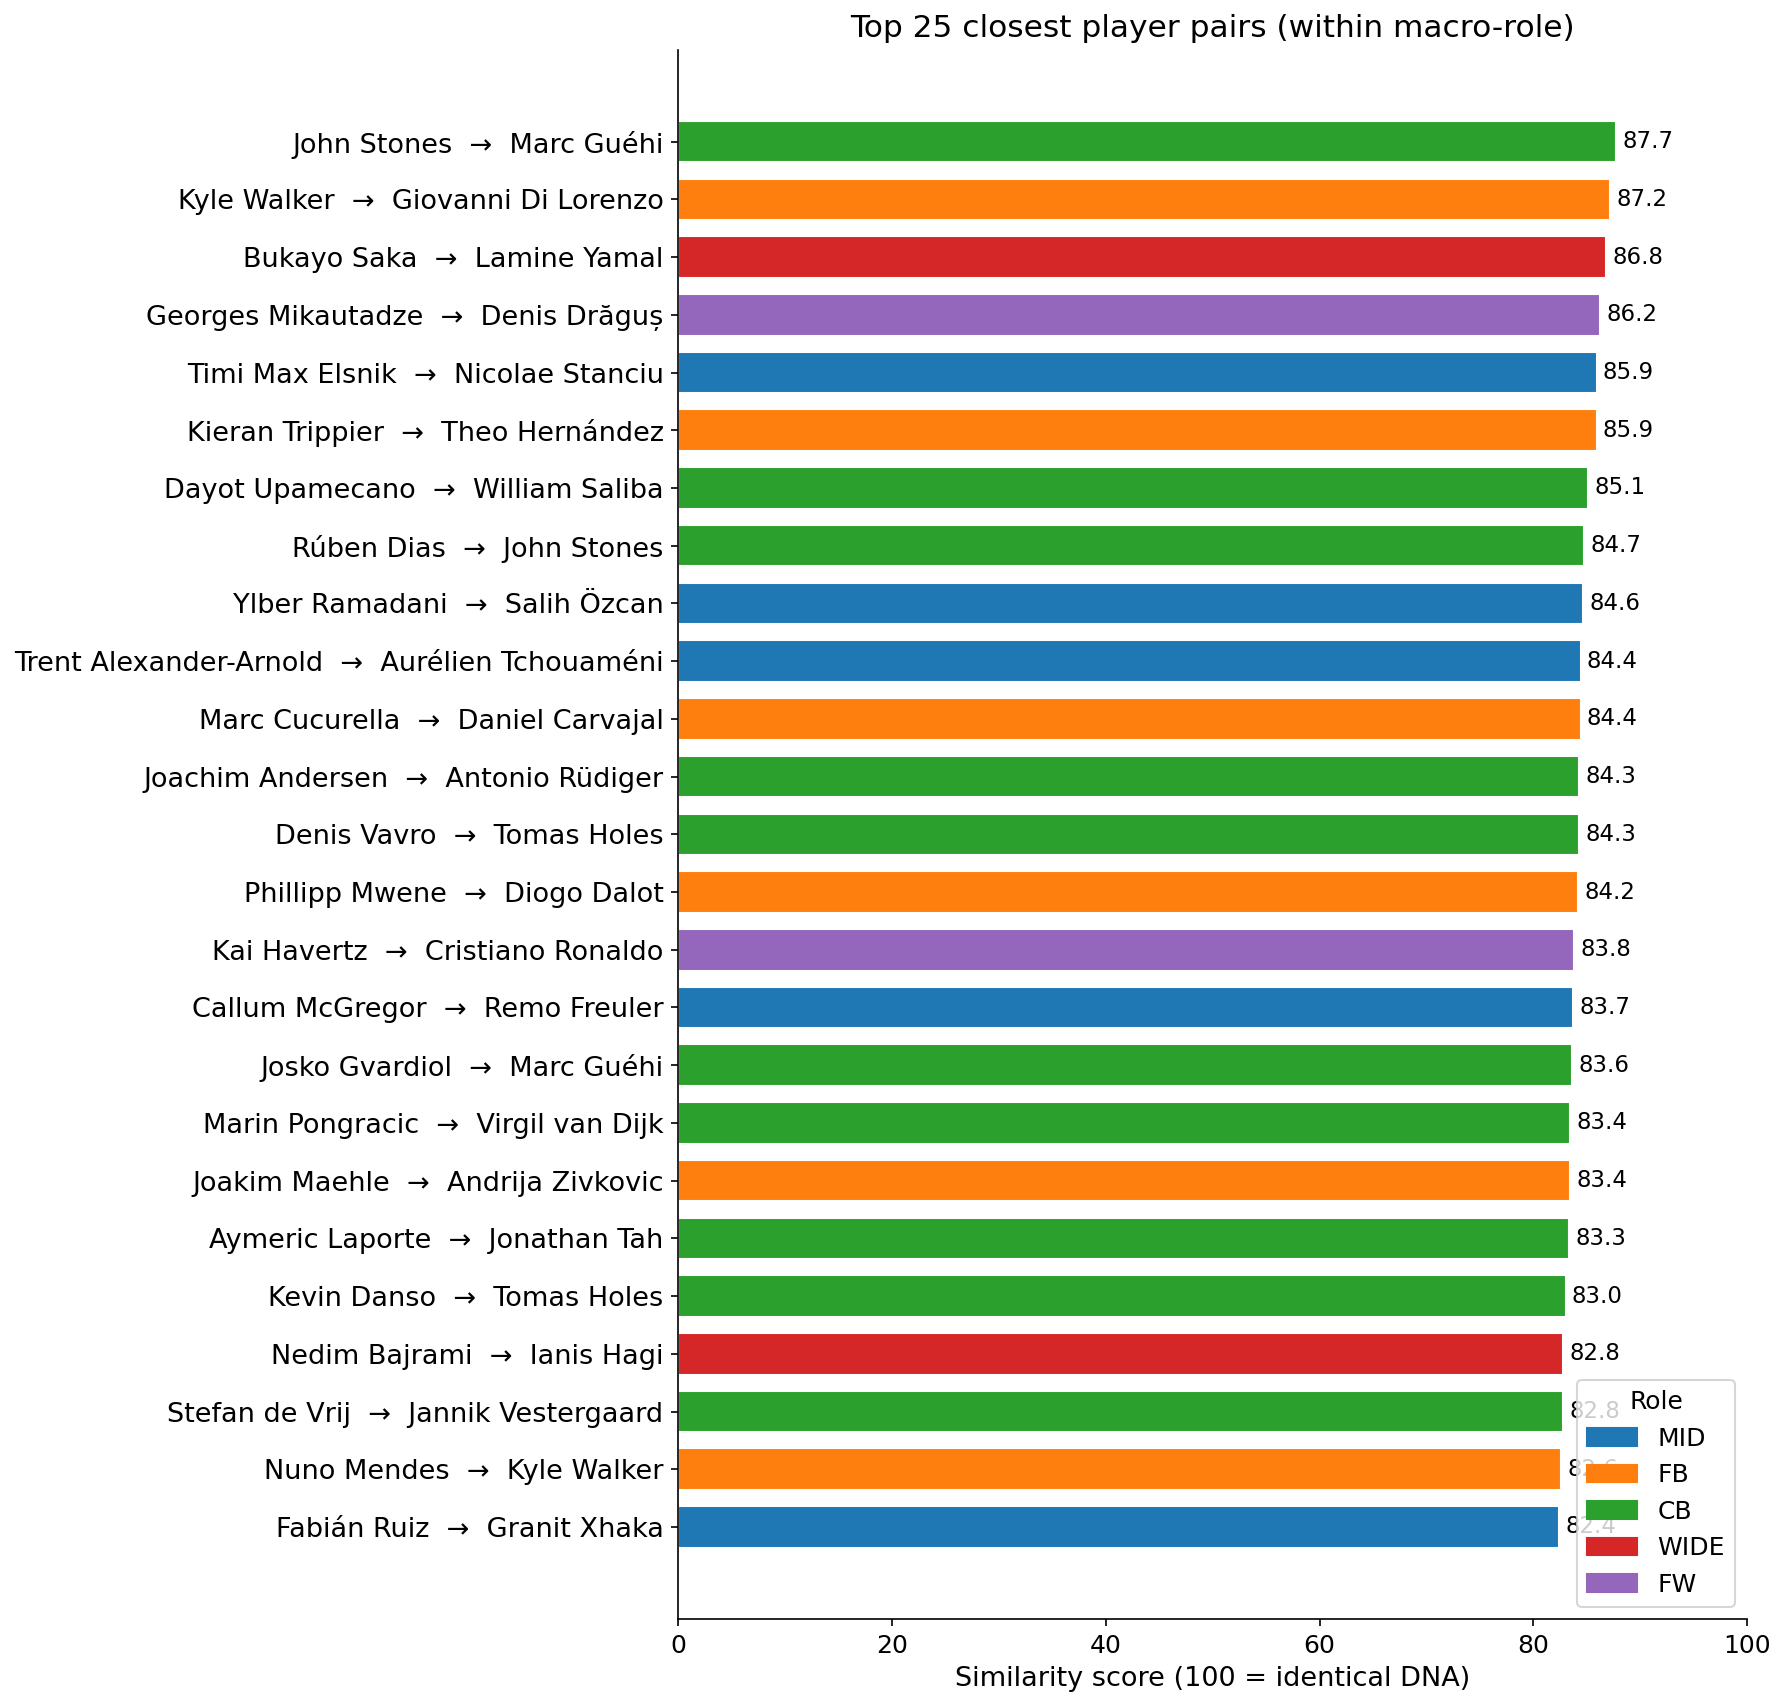
\includegraphics[width=0.92\textwidth]{images/top_pairs.png}
    \caption{The strongest within-role pairs in the pool, coloured by macro-role.  The scores top out near $88$ rather than at $100$, because two real footballers are never identical: a fixed maximum distance keeps the score absolute and comparable across pairs.  Every top pair is football-sensible (ball-playing centre-backs, attacking full-backs, elite wide dribblers), a direct face-validity check on the similarity metric.}\label{fig:h4-top-pairs}
\end{figure}

\subsection{Key Findings}\label{sec:h4-findings}

Each player's neighbour list reads as his stylistic family rather than merely his position.
Rodri (Spain, MID) sits next to other deep, controlling midfielders (Jorginho, Hjulmand, Kova\v{c}i\'{c}, Xhaka); Toni Kroos next to the metronomic passers (Tchou\'{a}meni, Zubimendi, Vitinha); Pedri and Bellingham next to the creative eights/tens (K\"{o}k\c{c}\"{u}, Eriksen, De Bruyne, G\"{u}ndoğan); R\"{u}diger and Bastoni next to the ball-playing centre-backs (Tah, Laporte, Andersen); Lamine Yamal next to the elite wide dribblers (Saka, Le\~{a}o, Williams, Dembélé).
The strongest pairs in the pool are all sensible (John Stones~$\leftrightarrow$~Marc Gu\'{e}hi at $87.7$, Kyle Walker~$\leftrightarrow$~Di Lorenzo at $87.2$, Lamine Yamal~$\leftrightarrow$~Saka at $86.8$).
On the value-arbitrage query, the cheaper look-alikes of Rodri (pre-Euro EUR\,120M) include Jorginho (similarity $82$, EUR\,12M), Granit Xhaka ($78$, EUR\,20M) and Morten Hjulmand ($81$, EUR\,40M), exactly the deep-lying alternatives a club could sign for a fraction of the price.

\begin{figure}[H]
    \centering
    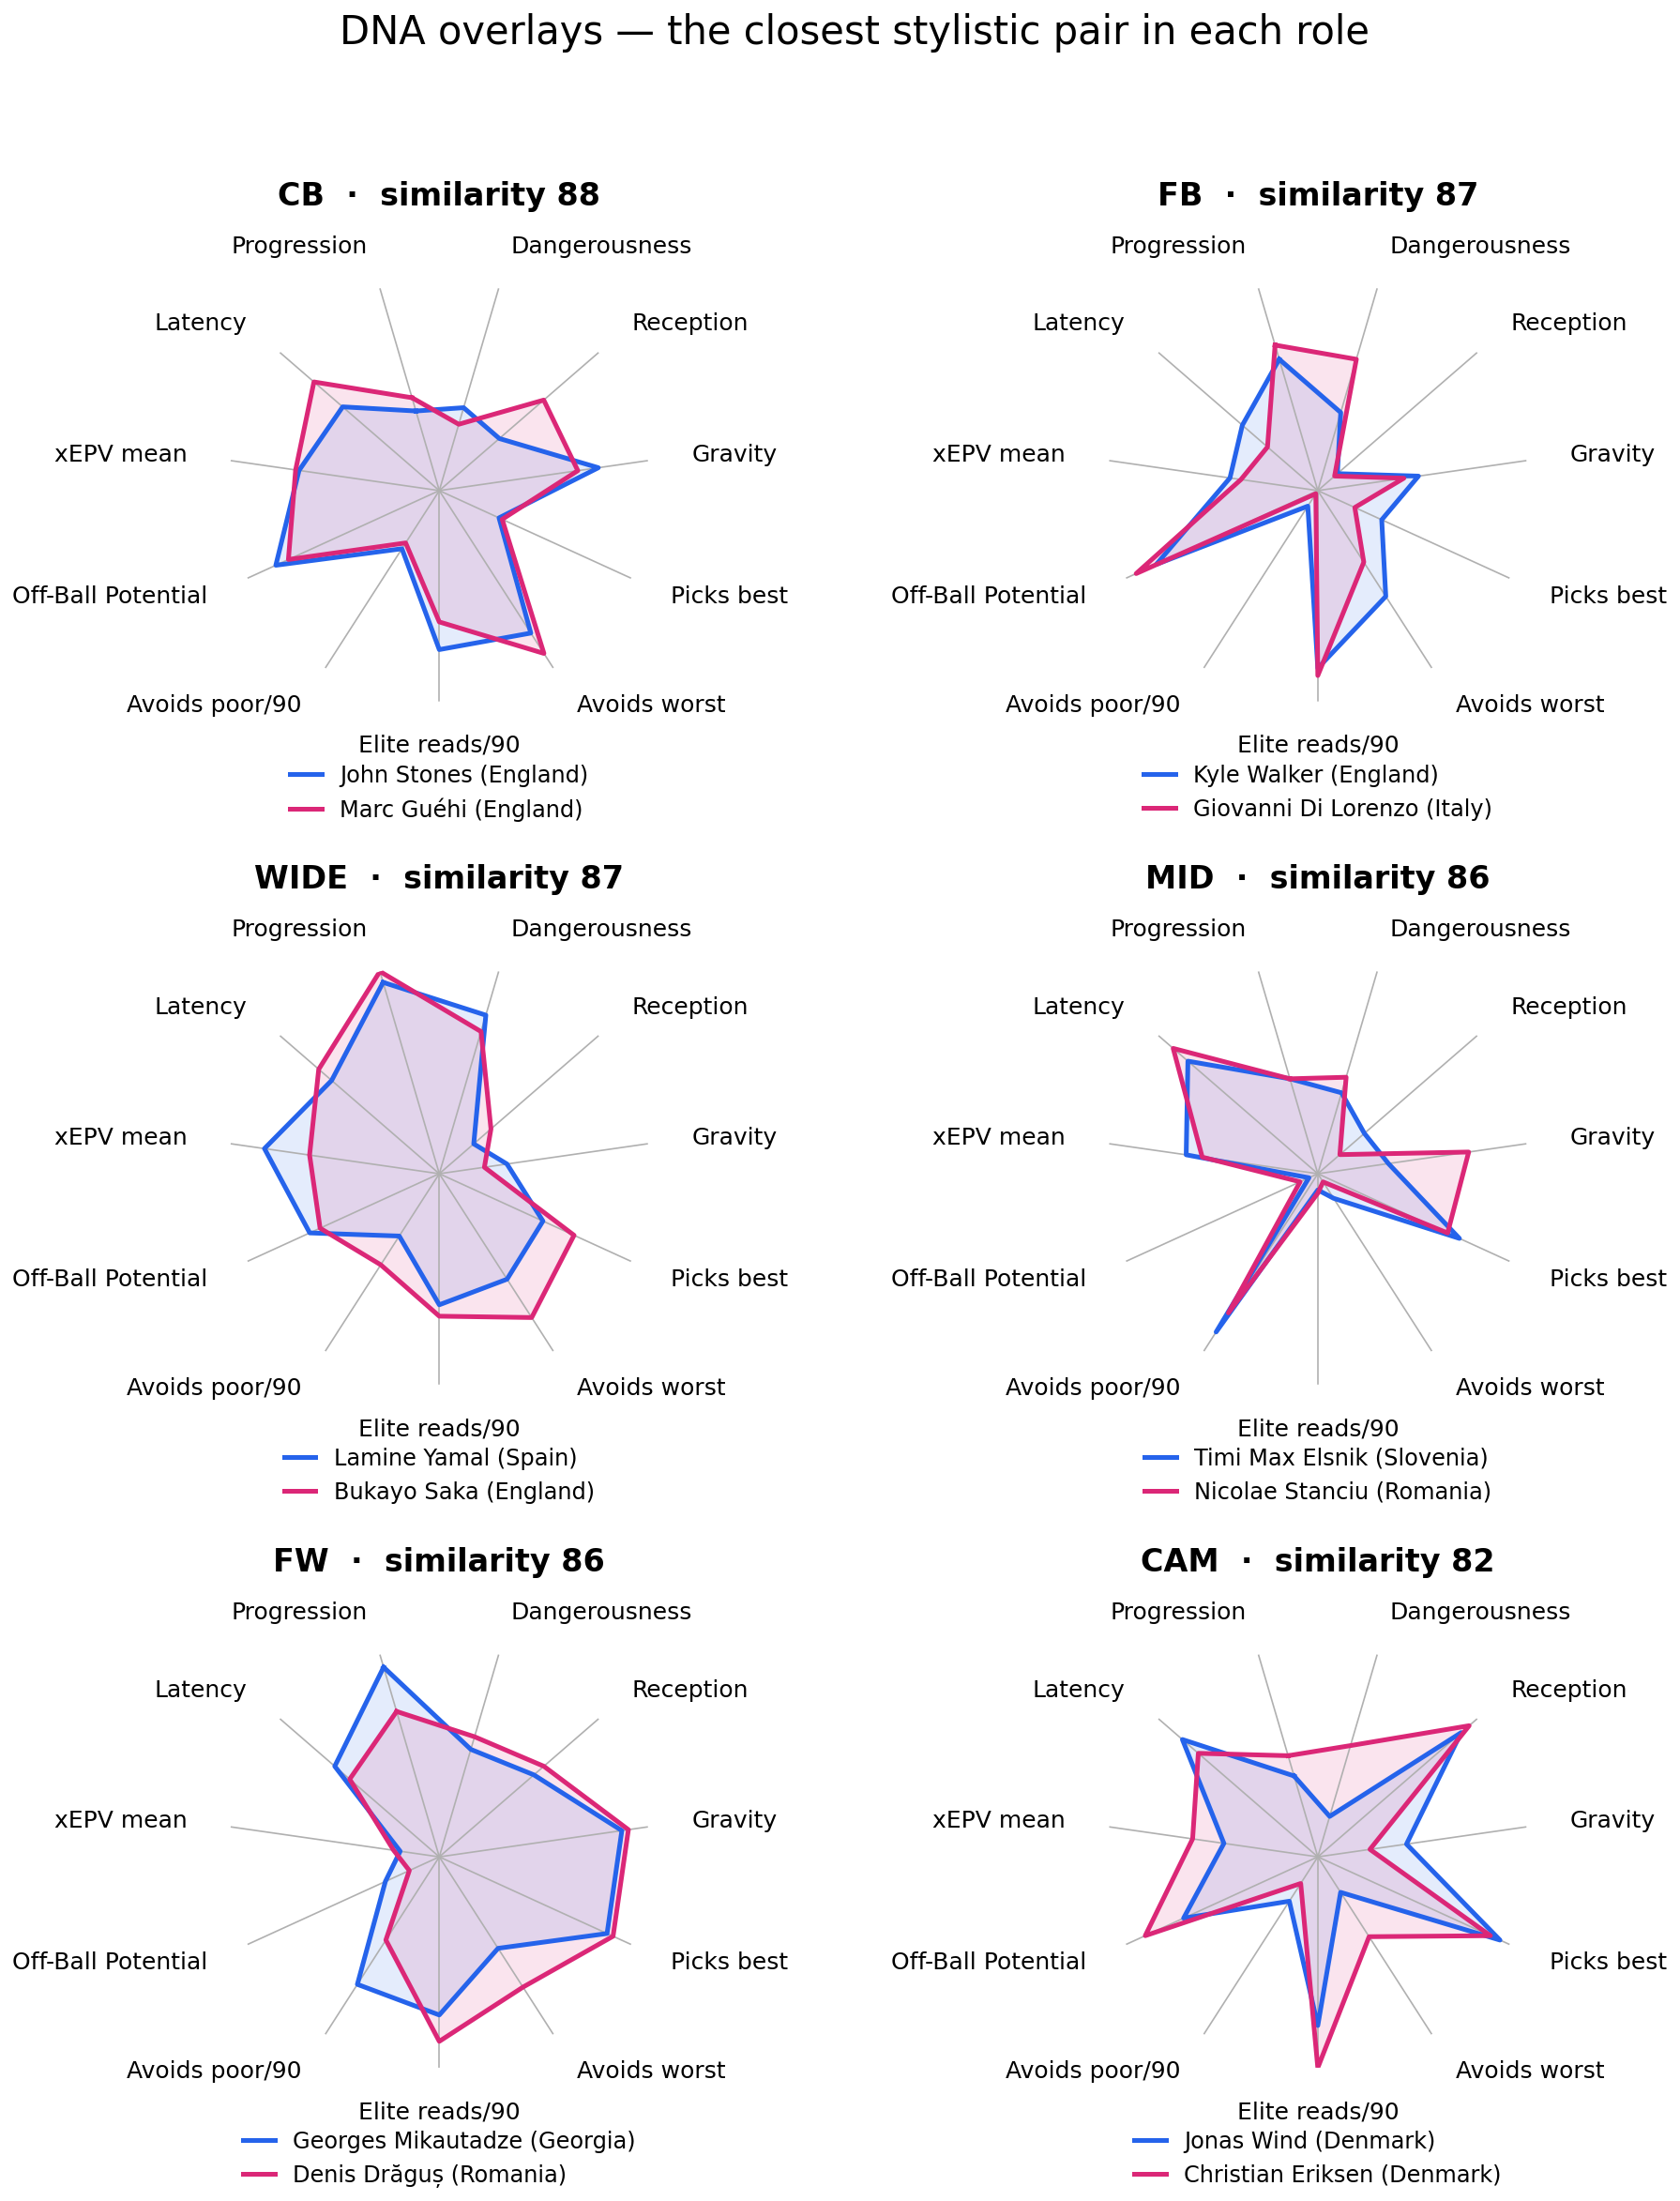
\includegraphics[width=\textwidth,height=0.8\textheight,keepaspectratio]{images/dna_overlay_by_role.png}
    \caption{DNA overlays: the closest stylistic pair in each macro-role, each player's 11-axis DNA drawn on the same radar.  The two polygons sit almost on top of each other, which is what a high similarity score looks like: the metric pairs John Stones with Marc Gu\'{e}hi (CB), Kyle Walker with Di Lorenzo (FB), Lamine Yamal with Saka (WIDE), and so on, recovering each player's stylistic family rather than merely his position.}\label{fig:h4-dna-overlay}
\end{figure}

\subsection{Integration with the Platform}\label{sec:h4-platform}

The dashboard already exposes a within-role player-comparison surface as the front end for the similarity model (\cref{sec:platform}).
With the similarity engine in place, the comparison page evolves from a manual head-to-head (where the scout picks two players) into an automated ``find me similar undervalued players'' query: each candidate's similarity score is presented alongside his market value and age, giving a single global read on a player's profile, namely how he plays, what he costs, and how old he is.

\clearpage
% ============================================================
\section{The Platform}\label{sec:platform}
% ============================================================

The four studies feed a single \textbf{interactive web dashboard}, the terminal deliverable of the project.
It is a contextual scouting tool: a scout can read a player's full contextual profile, run within-role head-to-heads, search the pool by attribute, and surface stylistically similar players against their market value.

\subsection{What a Scout Can Do}\label{sec:scout}

\begin{itemize}
    \item Read a player's profile: the H1, H2 and H3 cards side by side on one page. Every card follows the same pattern: a magnitude headline next to a within-role percentile radar that decomposes the profile behind it, with the raw scout-facing values shown underneath so low-sample profiles can be discounted.
    \item Run head-to-heads: two players of the same macro-role overlaid on the same radars, so the comparison always stays \emph{within role}. The picker prevents cross-role duels upstream, which keeps the comparison meaningful (a CB radar and a FW radar are not the same axes).
    \item Search by attribute: filter the pool by role, nationality and any contextual index, so a scout can ask for, say, the highest-Progression full-backs and shortlist them directly.
    \item Find similar players: the H4 engine returns a target's closest stylistic matches within his role, each shown next to his market value and age, which is the practical form of the value-arbitrage use case.
    \item Set performance against cost: the Transfermarkt market values let a scout read on-pitch contextual output against price, which is the value-arbitrage angle of the business case.
\end{itemize}

\subsection{Unified Card Design}\label{sec:card}

The card pattern is identical across the three on-pitch metrics (\cref{tab:cards}), which is what lets a scout read all three at a glance.

\begin{table}[H]
\centering
\caption{The unified card design.}\label{tab:cards}
\small
\begin{tabularx}{\textwidth}{@{}lLLL@{}}
\toprule
Metric & Headline & Radar & Axes \\
\midrule
H1 Dangerousness & EPV Added\,/\,90 pctile & spatial decomp. & 4 EPV-by-zone components \\ \midrule
H2 Decision Quality & DQ index pctile & behavioural decomp. & Picks-best, Avoids-worst, Elite\,/\,90, Avoids-poor\,/\,90 \\ \midrule
H3 Off-Ball & URS\,/\,90 pctile & exposure/usage decomp. & Potential\,/\,90, xEPV mean, Latency \\
\bottomrule
\end{tabularx}
\end{table}

In every case the radar polygon's shape tells the \emph{style}, the headline tells the \emph{magnitude}, and the raw block below guards against over-reading a thin sample.
All axes are oriented so that outside is better.

\subsection{Architecture}\label{sec:architecture}

The dashboard is a standard three-tier web application:
\begin{itemize}
    \item Frontend: React + TypeScript, with a player list and filters, a per-player profile holding the three metric sections, a within-role comparison page, an attribute search, a similar-players page, and a glossary that documents every metric for the end user.
    \item Backend: FastAPI (Python), which exposes the per-player metric endpoints.
    \item Database: Supabase / Postgres, loaded by a set of import scripts from the committed metric CSVs.
\end{itemize}
A data-cleaning and importing layer maps the StatsBomb player identities to the Transfermarkt profiles so the contextual metrics and the market values line up on the same player.

\clearpage
% ============================================================
\section{Reproducibility}\label{sec:reproducibility}
% ============================================================

The project is organised as a reproducible research artefact.
Each hypothesis lives in its own self-contained folder with its own dependencies (a per-study \texttt{requirements.txt}), a thin orchestrating notebook that imports all logic from a \texttt{src/} package, and committed output CSVs that allow an analysis-only path. A reader can open a notebook and jump straight to the index, validation and figure cells without re-running the heavy pipelines (the hull computation, the xPass training, or the resolver pull). Each folder also ships a dedicated \texttt{README} documenting that study's metric, its validation and its scout-facing findings, so a study can be read and re-run on its own.

The shared artefacts that H2, H3 and H4 inherit from H1 (the 272-player pool and the authoritative role assignment) are read-only, so the studies stay population-aligned.

Alongside the four studies, the market-value data is produced by a standalone Transfermarkt scraper (\cref{sec:transfermarkt}) that runs in a fixed order and updates incrementally, so re-running it never duplicates existing rows. The full repository, comprising the four studies, the Transfermarkt scraper and the interactive dashboard, is the primary deliverable alongside this paper.

\clearpage
% ============================================================
\section{Limitations and Declared Scope}\label{sec:limitations}
% ============================================================

Several limits are \emph{declared by design}: they are acknowledged inside the metric construction rather than discovered after the fact, which is a deliberate strength of the framework. They fall into three groups: limits of the 360 data itself, limits of the individual metrics, and limits of scope. The same list is surfaced to the end user on the dashboard, so a scout reading a profile sees exactly the caveats stated here.

\paragraph{Limits of the 360 data.}
These are properties of the freeze-frame source that no metric in this project can overcome.
\begin{enumerate}
    \item \textbf{A single instant, not a film.} Each metric reads the pitch at the \emph{moment the pass is played}, not the movement before it or the ball trajectory after. It describes the geometry of the decision, not how it unfolds: speed at reception, acceleration, distance covered and pressing intensity over time cannot be measured, and a player standing in a dangerous zone scores the same as one sprinting into it at that instant.

    \item \textbf{Pressure read from distance alone.} A frame shows where defenders are, not their physical state: a defender 2\,m away may be jogging or sprinting in to tackle, and the snapshot cannot tell them apart. The project-wide ``pressure'' definition (\cref{sec:conventions}) therefore approximates threat from distance only.

    \item \textbf{Partial player coverage.} A 360~frame usually shows only 8 to 12 of the 22 players, those near the ball; players far from the action are often missing. Anything measured far from the ball is correspondingly less reliable, which is one reason the off-ball resolver keeps only confident, ball-proximate assignments.

    \item \textbf{Anonymous opponents and teammates.} Only the player on the ball is named; everyone else carries just a team tag. The model therefore cannot weight opposition by \emph{quality}: beating a top defender counts the same as beating a weak one, and a pass into a dangerous zone is valued by the zone, not by who would actually receive or contest it.
\end{enumerate}

\paragraph{Limits of the individual metrics.}
\begin{enumerate}\setcounter{enumi}{4}
    \item \textbf{No game state.}\label{lim:game-state} xEPV is a per-pass quantity with no notion of scoreline, time remaining, match importance, or manager instruction. This is the source of the most counter-intuitive H2 reads: deliberate tempo controllers (Kimmich, Modric, Xhaka, Barella) sit below their role median because a deliberately safe, possession-securing pass reads as weak selection. The gap is the lens, not necessarily the player.

    \item \textbf{Not every visible option is a real choice (H2).} The DQ~index grades a pass against the \emph{in-frame} alternatives the resolver reconstructs, treating every reachable teammate as part of the decision set. Some in-frame options are technically available but tactically irrational (a square ball to the far-side full-back while breaking on the counter), yet they still enter the menu and inflate the Score. The framework already absorbs the converse case: every option is weighted by its own completion probability (xPass sits inside xEPV), and balls with no reachable receiver are dropped (the 12\,m pass-into-space filter), so unreachable options are down-weighted to near-zero value rather than rewarded. What remains unmodelled is \emph{tactical rationality}. For this reason the index is read as a relative choice-optimality measure within the model's reachable action set, not an absolute verdict on the pass.

    \item \textbf{Off-ball score depends on teammates too (H3).} A run counts toward URS only when it is not served, so part of the headline reflects how well a player's teammates see and execute the pass, not the player alone: a good mover surrounded by weaker passers can post a high score because his runs keep going unused. This is by design. The score splits into \textbf{Off-Ball Potential} (the value he exposes, a player-only measure) and \textbf{Latency} (the share left unserved, where teammates enter), and the two are nearly independent within role ($\rho \approx 0.08$); the environment effect is real but small ($\rho \approx -0.13$ between a player's Latency and his teammates' mean H2). Read Potential for the cleanest individual signal and the headline as off-ball value \emph{in his current team context}. So read, URS complements H2: one grades him as the passer, the other shows how often his own off-ball offers go unused.

    \item \textbf{Some things have no ground truth.} H2 compares the chosen pass against alternatives that were \emph{never actually played}, so there is no real outcome to check them against; the index limits the damage by only requiring the options to be ordered roughly right, not scored exactly. H3 has a similar gap: off-ball identities are reconstructed by estimating each anonymous teammate's position and matching it to his recent on-ball events. That is validated against StatsBomb's real pass recipient and reaches 93\% accuracy on the confident assignments it keeps (localised within 8\,m), far above the ${\sim}74\%$ naive baseline, but it remains an estimate, not a certainty, and dots it cannot place confidently are dropped, buying reliability at the cost of coverage.

    \item \textbf{Built on base models, shared across hypotheses.} The indices sit on top of an EPV grid (adapted from Friends of Tracking) and a custom \textbf{xPass} completion model (built for H2, reused by H3). Any error or assumption baked into these base layers carries through into every metric above them. And because H2, H3 and H4 read H1's player pool, role assignment and EPV from the \emph{same files}, a bias in those shared foundations would surface in all of them at once rather than as a disagreement between them.
\end{enumerate}

\paragraph{Limits of scope.}
\begin{enumerate}\setcounter{enumi}{9}
    \item \textbf{Single tournament, small samples.}\label{lim:single-tournament} All results are on Euro~2024 alone (51~matches), so patterns may not carry over to club football or other competitions; cross-tournament generalisation is validated only for internal stability (split-half, robustness), not across datasets. Players need at least 135~minutes ($\approx 1.5$~matches) to enter, and the per-role pools are small, so a low-sample player has a noisy ranking that can also nudge the players around him. The sample size is always shown next to the headline so low-sample profiles can be discounted. Relatedly, the six macro-role pools differ in size, so a percentile in a small pool (e.g.\ CAM, $n=20$) is a coarser rank than one in a large pool.

    \item \textbf{Team bias reduced, not removed.} Grading players by the \emph{value} of what they do rather than the \emph{volume}, then ranking them within role, removes most of the team bias that distorts raw statistics. What it cannot remove is exposure: a player in a possession-dominant side still appears in more freeze frames, and gets more chances to add value, than an equal player in a pressed side. This residual is the honest boundary of the whole approach, and it is why the absolute off-ball leaderboard is midfield-heavy and must be read within role.
\end{enumerate}

\clearpage
% ============================================================
\section{Future Work}\label{sec:future}
% ============================================================

\subsection{AI Scouting Report}\label{sec:ai-report}

The project proposal scopes, as a stretch goal, an AI-driven reporting module that translates the contextual metrics into concise, readable scouting reports, turning a player's radars and raw blocks into prose a scout can act on.
This is future work and is not part of the current deliverable.

\subsection{Other Directions}\label{sec:other-future}

Each direction below addresses a specific limit declared in \cref{sec:limitations}.
\begin{itemize}
    \item Game state in xEPV: conditioning the value layer on scoreline and game phase, which would close the tempo-controller blind spot of \cref{lim:game-state} (the main H2 scope limit, where deliberately safe passing reads as weak selection).
    \item Cross-tournament validation: re-running the four metrics on other StatsBomb 360 competitions to test generalisation beyond Euro~2024, directly addressing \cref{lim:single-tournament}.
    \item Defensive off-ball value: H3 currently measures \emph{offensive} off-ball exposure; the mirror concept (the dangerous space a player \emph{denies} the opponent) is a natural extension.
    \item Combined player-plus-fit score: quantifying the H2 $\times$ H3 pairing into a single score that captures both the player's decision quality and how well his off-ball value is used by his current team.
    \item Richer player similarity (H4): H4 currently compares players within role on an 11-axis DNA. Natural extensions are cross-league matching (finding Euro look-alikes in club competitions, the practical scouting query), learned axis weights instead of the present equal weighting, and validating the matches and the value-arbitrage shortlist against realised market-value and on-pitch outcomes once multi-tournament data is available (which depends on \cref{lim:single-tournament}).
\end{itemize}

\clearpage
% ============================================================
\section{Conclusion}\label{sec:conclusion}
% ============================================================

Traditional scouting statistics reward volume and carry a structural team bias that flatters players in dominant sides.
This project reframes player evaluation around \emph{what a player does with the space around him}, graded by value (EPV) rather than volume, and benchmarked within role rather than against the whole pitch.

Four completed and independently validated studies implement this thesis:
\begin{itemize}
    \item Space Control (four spatial-influence indices),
    \item \textbf{Decision Quality} (the value of the chosen pass relative to the options ignored),
    \item \textbf{Off-Ball Movement} (the dangerous off-ball space teammates fail to use),
    \item \textbf{Player Similarity} (matching players within role by contextual ``spatial DNA'' for value arbitrage).
\end{itemize}

The evidence is consistent and pointed: ball volume is a poor proxy for value created. On the EPV-creation index, more than half the pool moves by $20+$~percentile points when shifting from a volume ranking to a contextual one. The off-ball metric also isolates a genuine, previously invisible signal, representing the shadow runner who keeps offering dangerous options their team does not use, with Pedri the clearest case at the tournament.

Read together, the six contextual axes (the four H1 indices, plus H2 Decision Quality and H3 off-ball rating) also show which players have \emph{no weak side}. Asking a player to clear the 50th within-role percentile on \emph{all six} at once leaves only five in the whole pool: Mateo Kova\v{c}i\'{c} (Croatia, MID), Florian Wirtz (Germany, WIDE), Kevin De Bruyne (Belgium, CAM), Adrien Rabiot (France, MID) and Milan \v{S}kriniar (Slovakia, CB), the only centre-back among them. We do not read this as a ranking of the best players at the tournament; it rests on a single competition and the test is a simple one. We read it as a sign that the six axes measure different things: if they overlapped, many more players would clear all six together, and the fact that so few do shows that the profile separates players rather than describing the same quality six times.

The four metrics are unified in an interactive scouting dashboard that lets a scout read a player's full contextual profile, run within-role comparisons, and (with the similarity model) discover undervalued alternatives.
The framework is built to be honest about its own limits, and each sets up a clear next step: game-state-aware value models, cross-tournament validation, defensive off-ball value, richer cross-league similarity, and AI-generated scouting reports.

% ============================================================
% REFERENCES
% ============================================================

\clearpage
\begin{thebibliography}{9}
\sloppy

\bibitem{statsbomb}
StatsBomb.
\emph{StatsBomb Open Data}.
UEFA Euro 2024 (\texttt{competition\_id\,=\,55}, \texttt{season\_id\,=\,282}), 51 matches.
\url{https://github.com/statsbomb/open-data}

\bibitem{epv}
Friends of Tracking.
\emph{Expected Possession Value (EPV) grid and tutorials}.
\url{https://github.com/Friends-of-Tracking-Data-FoTD}.

\bibitem{transfermarkt}
Transfermarkt.
\emph{Market values for UEFA Euro 2024 participants}.
Scraped via the project's own incremental pipeline.

\bibitem{hungarian}
Kuhn, H.\,W.
\emph{The Hungarian method for the assignment problem}.
Naval Research Logistics Quarterly, 2(1--2):83--97, 1955.

\bibitem{shap}
Lundberg, S.\,M.\ and Lee, S.-I.
\emph{A Unified Approach to Interpreting Model Predictions}.
Advances in Neural Information Processing Systems, 30, 2017.

\bibitem{xt}
Singh, K.
\emph{Introducing Expected Threat (xT)}.
2019. \url{https://karun.in/blog/expected-threat.html}

\bibitem{pitchcontrol}
Spearman, W.
\emph{Beyond Expected Goals}.
MIT Sloan Sports Analytics Conference, 2018.

\bibitem{vaep}
Decroos, T., Bransen, L., Van Haaren, J., and Davis, J.
\emph{Actions Speak Louder than Goals: Valuing Player Actions in Soccer (VAEP)}.
ACM SIGKDD International Conference on Knowledge Discovery \& Data Mining, 2019.

\bibitem{packing}
Reinartz, S.\ and Hegeler, J.
\emph{Packing: a metric for defenders bypassed by a pass}.
IMPECT GmbH.

\end{thebibliography}

% ============================================================
% FIGURE INDEX (Appendix)
% ============================================================
\clearpage
\appendix
\section{Figure Index}\label{app:figures}

All figures are stored in \texttt{docs/paper/images/} and originate from the hypothesis pipelines' \texttt{docs/figures/} folders.

\begin{table}[H]
\centering
\caption{Figures used in this paper.}\label{tab:figures}
\small
\begin{tabularx}{\textwidth}{@{}lLll@{}}
\toprule
Figure & File & Origin & Section \\
\midrule
\cref{fig:h1-radar} & \texttt{h1\_radar\_kimmich.png} & H1 card & \cref{sec:h1-findings} \\ \midrule
\cref{fig:scouting-discoveries} & \texttt{scouting\_discoveries.png} & H1 validation & \cref{sec:h1-findings} \\ \midrule
\cref{fig:naive-overrating} & \texttt{naive\_overrating.png} & H1 validation & \cref{sec:h1-findings} \\ \midrule
\cref{fig:kroos-frame}a & \texttt{xpass\_example.png} & H2 xPass & \cref{sec:dq-example} \\ \midrule
\cref{fig:kroos-frame}b & \texttt{xepv\_example.png} & H2 xEPV & \cref{sec:dq-example} \\ \midrule
\cref{fig:dq-radar} & \texttt{dq\_radar\_example.png} & H2 radar & \cref{sec:dq-radar} \\ \midrule
\cref{fig:within-role-top5} & \texttt{within\_role\_top5.png} & H3 roles & \cref{sec:h3-findings} \\ \midrule
\cref{fig:h2h} & \texttt{h2h\_pedri\_kroos.png} & H3 h2h & \cref{sec:h3-findings} \\ \midrule
\cref{fig:offball-pedri} & \texttt{offball\_radar\_pedri.png} & H3 radar & \cref{sec:h3-findings} \\ \midrule
\cref{fig:uncap-pedri} & \texttt{uncapitalised\_runs\_pedri.png} & H3 visual proof & \cref{sec:h3-findings} \\ \midrule
\cref{fig:archetype-map} & \texttt{archetype\_map.png} & H3 archetypes & \cref{sec:h3-findings} \\ \midrule
\cref{fig:h4-top-pairs} & \texttt{top\_pairs.png} & H4 validation & \cref{sec:h4-validation} \\ \midrule
\cref{fig:h4-dna-overlay} & \texttt{dna\_overlay\_by\_role.png} & H4 findings & \cref{sec:h4-findings} \\
\bottomrule
\end{tabularx}
\end{table}

\end{document}
